%
\providecommand{\main}{../..}
\documentclass[12pt,a4paper]{report}


%---General---%
\usepackage{subfiles} %Modular structure
\usepackage[ddmmyyyy,hhmmss]{datetime} %Compilation date
\usepackage[english]{babel}
\usepackage{microtype}
\usepackage[nointegrals]{wasysym} %fonts support
\usepackage[a4paper,inner=20mm,outer=49mm,top=20mm,bottom=25mm,%
            marginparsep=6mm,marginparwidth=30mm]{geometry}

\newcommand\hmmax{0} %Avoid too many alphabets error
\newcommand\bmmax{0}
\renewcommand{\rmdefault}{ppl} % rm
\linespread{1.05}        % Palatino needs more leading
\usepackage[scaled]{helvet} % ss
\usepackage{courier} % tt
\usepackage{mathpazo} 

%---Encoding---%
\usepackage[utf8]{inputenc}
\usepackage[T1]{fontenc}
\usepackage{lmodern}
\usepackage{csquotes}

%---Math---%
\usepackage{amsmath,amsthm,amstext,amsbsy,amsfonts,amssymb,stackengine}
\usepackage{mathrsfs}
\usepackage{cancel}
\usepackage{bm}
\usepackage{mathtools}
\usepackage{mathdots}
\usepackage{thmtools}
\usepackage{array}
\usepackage{yhmath}
\usepackage{gensymb}
\usepackage{blkarray}

\newcommand\myop{\ensuremath\mathrel{\raisebox{1pt}{\stackunder{$<$}{\rotatebox{-27}{\resizebox{7pt}{2pt}{$\sim$}}}}}}
\setstackgap{S}{-1.5pt}
%---Physics---%
\usepackage{physics}
\usepackage{siunitx}
\sisetup{
separate-uncertainty = true
}
%\usepackage{braket}
%\usepackage[version=4]{mhchem}
%\usepackage{hepnames}

%---Tables---%
\usepackage{booktabs}
\usepackage{multirow}

\setlength{\aboverulesep}{0pt} %removes annoying spaces in booktabs tables
\setlength{\belowrulesep}{0pt}
\setlength{\extrarowheight}{.75ex}
\setlength\parindent{0pt} 

%---Graphics & Plots---%
\usepackage{graphicx}
\usepackage[usenames, dvipsnames, table]{xcolor} %colori
\usepackage{color}
\usepackage{wrapfig}

\usepackage[font=footnotesize, labelfont=bf,
            labelformat=parens,
            labelsep=endash, justification=raggedright,
            singlelinecheck=on]{caption} %fancy captions
\usepackage{subcaption} 
% \captionsetup[sub]{font=footnotesize,
%             labelsep=endash, justification=centering}

\usepackage{pgf,tikz}
\usetikzlibrary{arrows}
\usetikzlibrary{tikzmark}
\usetikzlibrary{patterns}
\usepackage{soul}
\usepackage[framemethod=tikz]{mdframed}
\usepackage{fancybox}
\usepackage{framed}

%---(Inkscape imports)---%
\usepackage{import}
\usepackage{xifthen}
\usepackage{pdfpages}
\usepackage{transparent}

\newcommand{\incfig}[1]{%
    \def\svgwidth{\columnwidth}
    \import{./figures/}{#1.pdf_tex}
}

\definecolor{mygray}{gray}{0.6}


%---Indeces, links, bibliography---%
\usepackage{imakeidx} %Indice analitico
\usepackage[stable]{footmisc}

%\usepackage{xr-hyper}
\PassOptionsToPackage{hyphens}{url}\usepackage{hyperref}  %hyperref va caricato sempre dopo footmisc, altrimenti le footnotes si buggano e riportano tutte alla prima pagina
\usepackage[inline]{showlabels} %Draft

\usepackage[symbol=$\wedge$,numberlinked=false]{footnotebackref}
\makeindex[columns=2, title=Analytical index, options= -s indexstyle.ist]

\usepackage[backend=biber,sorting=none]{biblatex}
\renewbibmacro{in:}{}
\addbibresource{bibliography.bib}

%---Utilities---%
\usepackage{comment}
\usepackage{xspace}
\usepackage{marginnote}
\usepackage{ragged2e}
\usepackage{enumerate}
\usepackage{enumitem}
\usepackage{etoolbox}
\usepackage{xargs}                      % Use more than one optional parameter in a new commands
\usepackage{lipsum}  
\usepackage{float}

%---Additional symbols---%
%\bigcdot
\makeatletter
\newcommand*\bigcdot{\mathpalette\bigcdot@{.5}}
\newcommand*\bigcdot@[2]{\mathbin{\vcenter{\hbox{\scalebox{#2}{$\m@th#1\bullet$}}}}}
\makeatother

%Circled symbols
\makeatletter
\newcommand{\ogeneric}[2][0.7]{%
  \vphantom{\oplus}\mathpalette\o@generic{{#1}{#2}}%
}
\newcommand{\o@generic}[2]{\o@@generic#1#2}
\newcommand{\o@@generic}[3]{%
  \begingroup
  \sbox\z@{$\m@th#1\oplus$}%
  \dimen@=\dimexpr\ht\z@+\dp\z@\relax
  \savebox\tw@[\totalheight]{$\m@th#1\bigcirc$}%
  \makebox[\wd\z@]{%
    \ooalign{%
      $#1\vcenter{\hbox{\resizebox{\dimen@}{!}{\usebox\tw@}}}$\cr
      \hidewidth
      $#1\vcenter{\hbox{\resizebox{#2\dimen@}{!}{$#1\vphantom{\oplus}{#3}$}}}$%
      \hidewidth
      \cr
    }%
  }%
  \endgroup
}
\makeatother

\newcommand{\ole}{\mathrel{\ogeneric{<}}} 
\newcommand{\oleq}{\mathrel{\ogeneric[0.6]{\leq}}}
\newcommand{\osubseteq}{\mathrel{\ogeneric[0.6]{\subseteq}}}
\newcommand{\thickfrac}[2]{\genfrac{}{}{1.1pt}{}{\displaystyle #1}{\displaystyle #2}}

%---New environments---%
%Exercises + Examples
\newenvironment{myleftbar}{%
\def\FrameCommand{\hspace{0.6em}\vrule width 2pt\hspace{0.6em}}%
\MakeFramed{\advance\hsize-\width \FrameRestore}}%
{\endMakeFramed}
\declaretheoremstyle[
spaceabove=6pt,
spacebelow=6pt
headfont=\normalfont\bfseries,
headpunct={} ,
headformat={\cornersize*{2pt}\ovalbox{\NAME~\NUMBER\ifstrequal{\NOTE}{}{\relax}{\NOTE}:}},
bodyfont=\normalfont,
]{exobreak}

\declaretheorem[style=exobreak, name=Exercise,%
numberwithin = section, %
postheadhook=\leavevmode\myleftbar, %
prefoothook = \endmyleftbar]{exo}

%show just the name in theorem list
\makeatletter
%\show\ll@problem gives default definition:
% \protect \numberline {\csname the\thmt@envname \endcsname }\thmt@thmname \ifx
% \@empty \thmt@shortoptarg \else \protect \thmtformatoptarg {\thmt@shortoptarg 
% }\fi
\def\ll@exo{%
  \protect\numberline{\theexo}\thmt@shortoptarg%
}
\makeatother

\usepackage[type={CC}, lang=english, modifier={by-nc-sa}, version={4.0}]{doclicense}
%Chapter division in theorem list
%\colorlet{shadecolor}{lightgray!25}

\usepackage{etoolbox}
\makeatletter
\patchcmd\thmtlo@chaptervspacehack
  {\addtocontents{loe}{\protect\addvspace{10\p@}}}
  {\addtocontents{loe}{\protect\thmlopatch@endchapter\protect\thmlopatch@chapter{\thechapter}}}
  {}{}
\AtEndDocument{\addtocontents{loe}{\protect\thmlopatch@endchapter}}
\long\def\thmlopatch@chapter#1#2\thmlopatch@endchapter{%
  \setbox\z@=\vbox{#2}%
  \ifdim\ht\z@>\z@
    \hbox{\bfseries\chaptername\ #1}\nobreak
    #2
    \addvspace{10\p@}
  \fi
}
\def\thmlopatch@endchapter{}

\makeatother
\renewcommand{\thmtformatoptarg}[1]{ -- #1}
\renewcommand{\listtheoremname}{List of definitions}
%%%

\declaretheorem[style=exobreak, name=Example,%
postheadhook=\leavevmode\myleftbar, %
prefoothook = \endmyleftbar]{example}

\usepackage{etoolbox}
\usepackage{needspace}
\AtBeginEnvironment{exo}{\Needspace{10\baselineskip}}% Impedisce l'inserimento di una domanda a fondo pagina e la risposta alla pagina successiva
\AtBeginEnvironment{example}{\Needspace{10\baselineskip}}

%---Custom commands---%
\newcommand{\q}[1]{``#1''}              %quotes
\newcommand{\hlc}[2]{%
  \colorbox{#1!50}{$\displaystyle#2$}}  %highlight
\newcommand{\bb}[1]{\mathbb{#1}}        %faster \mathbb
\newcommand{\breakpage}{\begin{center}
  $\ast$~$\ast$~$\ast$
\end{center}}                           %fancy page separator
\newcommand{\lesson}[2]{\marginpar{(Lesson #1 of #2)\\Compiled: \today}}  %Lesson number, date and compilation

%---Dots---%
\newcommand{\danger}{{\textcolor{Red}{\fontencoding{U}\fontfamily{futs}\selectfont\char 66\relax}}}
\newcommand{\reddot}{\href{http://bit.ly/2Tj5OEj}{\tikz\draw[red,fill=red] (0,0) circle (.5ex);}}
\newcommand{\bluedot}{\href{\tikz\draw[blue,fill=blue] (0,0) circle (.5ex);}{http://bit.ly/2Tj5OEj}}
\newcommand{\greendot}{\href{http://bit.ly/2Tj5OEj}{\tikz\draw[green,fill=green] (0,0) circle (.5ex);}}
\newcommand{\orangedot}{\href{http://bit.ly/2Tj5OEj}{\tikz\draw[orange,fill=orange] (0,0) circle (.5ex);}}


%---Fancy stuff---%
%\usepackage[Bjornstrup]{fncychap}
%\usepackage{fancyhdr}
%\pagestyle{fancy}
%\fancyhead{} % clear all header fields
%\renewcommand{\headrulewidth}{0pt} % no line in header area
%\fancyfoot{} % clear all footer fields
%\fancyfoot[R]{A.A. 2018/19} % other info in "inner" position of footer line
%\cfoot{\thepage}

\makeatletter
\def\thickhrulefill{\leavevmode \leaders \hrule height 1ex \hfill \kern \z@}
\def\@makechapterhead#1{%
  \vspace*{10\p@}%
  {\parindent \z@ \raggedleft \reset@font
            \scshape \@chapapp{} \thechapter
        \par\nobreak
        \interlinepenalty\@M
    \Huge \bfseries #1\par\nobreak
    %\vspace*{1\p@}%
    \hrulefill
    \par\nobreak
    \vskip 100\p@
  }}
\def\@makeschapterhead#1{%
  \vspace*{10\p@}%
  {\parindent \z@ \raggedleft \reset@font
            \scshape \vphantom{\@chapapp{} \thechapter}
        \par\nobreak
        \interlinepenalty\@M
    \Huge \bfseries #1\par\nobreak
    %\vspace*{1\p@}%
    \hrulefill
    \par\nobreak
    \vskip 100\p@
  }}

%---Theorems---%
\theoremstyle{plain}
\newtheorem{thm}{Theorem}[section]
\newtheorem{lem}{Lemma}[section]
\newtheorem{prop}{Proposition}[section]
\newtheorem{axi}{Axiom}
\newtheorem{pst}{Postulato}

\theoremstyle{definition}
\newtheorem{dfn}{Definition}

%---Colored blocks---%
\newenvironment{expl}{\begin{mdframed}[hidealllines=true,backgroundcolor=green!20,innerleftmargin=3pt,innerrightmargin=3pt,leftmargin=-3pt,rightmargin=-3pt]}{\end{mdframed}} %Box di colore verde
\newenvironment{appr}{\begin{mdframed}[hidealllines=true,backgroundcolor=blue!10,innerleftmargin=3pt,innerrightmargin=3pt,leftmargin=-3pt,rightmargin=-3pt]}{\end{mdframed}} %Approfondimenti matematici (box di colore blu)

%Raggedright marginpar
\makeatletter
\renewcommand{\@marginparreset}{%
  \reset@font\footnotesize
  \raggedright
  \slshape
  \@setminipage
}
\makeatother


\allowdisplaybreaks %allow pagebreaks in align enviroments

\newgeometry{total={170mm,257mm}, left=20mm, top=20mm}
\begin{document}

\chapter{Complex Systems Exercises}


\begin{exo}[Ising Model]
    Consider a $1$-dimensional Ising Model with nearest-neighbour ferromagnetic interaction in an external uniform field with energy function given by:
    \begin{align*}
        \mathcal{H}(\bm{\sigma}) = -J \sum_{x=1}^N \sigma_x \sigma_{x+1} - B \sum_{x=1}^N \sigma_x \qquad J > 0
    \end{align*}    
    where periodic boundary conditions are used, i.e. $\sigma_{N+1} \equiv \sigma_1$. Define $K \equiv \beta J$ and $h \equiv \beta B$.
    
    \medskip
    
    \textbf{Part A}. Using the transfer matrix $\mathrm{T}(\sigma, \sigma') = \exp(K \sigma \sigma' + h (\sigma + \sigma')/2)$ and its spectral decomposition, determine:
    \begin{enumerate}
        \item The \textbf{partition function} $Z(K,h)$
        \item The \textbf{free energy} per node in the thermodynamic limit and its plot for $h=0$ versus $1/K$
        \item The \textbf{entropy} per node in the thermodynamic limit and its plot for $h=0$ versus $1/K$
        \item The \textbf{mean energy} per node in the thermodynamic limit and its plot for $h=0$ versus $1/K$
        \item The \textbf{specific heat} per node in the thermodynamic limit and its plot for $h=0$ versus $1/K$
        \item The \textbf{average magnetization} at $x$, $\langle \sigma_x \rangle$, in the thermodynamic limit and its plot for $h=0, 0.1, 0.2, 0.5, 1$ versus $1/K$ and for $K=1$ versus $h$ in the range $(-5,5)$
        \item The \textbf{two-point correlation function} $\langle \sigma_x \sigma_{x+y} \rangle$ in the thermodynamic limit and its plot for $h=0$ and $K=1$ versus $y$.
    \end{enumerate}

    \textbf{Part B}. Consider the same model with \textbf{open} boundary conditions (node $1$ is linked only to node $2$, and node $N$ only to node $N-1$):
    \begin{align*}
        \mathcal{H}(\bm{\sigma}) = -J \sum_{x=1}^{N-1} \sigma_x \sigma_{x+1} - B \sum_{x=1}^N \sigma_x
    \end{align*}   
    Show that the partition function for this case can be formally written as:
    \begin{align*}
        Z(K,h) = \bm{v}^T \mathrm{T}^N \bm{v} \equiv \sum_{\substack{\sigma_1 = \pm 1\\ \sigma_N = \pm 1}} v(\sigma_1) \mathrm{T}^N(\sigma_1, \sigma_N) v(\sigma_N)  
    \end{align*}
    where $v(\sigma) = e^{h \sigma /2}$. Show that the free energy per node in the thermodynamic limit is the same as above.
    
    \medskip

    \textbf{Part C}. Same as in part $B$ with fixed boundary conditions $\sigma_1 = 1 = \sigma_N$, and $v(\sigma) = e^{h/2}$ for both $\sigma=\pm 1$.
    
    \medskip

    \textbf{Part D}. How would you try to solve the Ising model in $1$-dimension with nearest neighbour and next-to-nearest neighbour interaction and periodic boundary condition ($\sigma_{N+1} = \sigma_1$ and $\sigma_{N+2} = \sigma_2$):
    \begin{align*}
        \mathcal{H}(\bm{\sigma}) = -\sum_{x=1}^N (J_1 \sigma_x \sigma_{x+1} + J_2 \sigma_x \sigma_{x+2}) - B \sum_{x=1}^N \sigma_x
    \end{align*} 

\end{exo}

\section{Solution}
    \subsection{Part A}

    Consider a $d=1$ system with $N$ spins. The periodic boundary conditions are $\sigma_{N+1} = \sigma_1$.
    \begin{enumerate}
        \item The \textbf{partition function} is given by:
        \begin{align*}
            Z(K,h) &= \sum_{\{\bm{\sigma}\}} e^{-\beta \mathcal{H}(\bm{\sigma})} = \sum_{\{\bm{\sigma}\}} \exp\left(K \sum_{x=1}^N \sigma_x \sigma_{x+1} + h \sum_{x=1}^N \sigma_x\right) =\\
            &= \sum_{\{\bm{\sigma}\}} \prod_{x=1}^N \underbrace{\exp\left(K \sigma_x \sigma_{x+1} + h \frac{\sigma_x + \sigma_{x+1}}{2} \right)}_{\mathrm{T}_{\sigma_x,\sigma_{x+1}}}  =\\
            &= \sum_{\sigma_1 = \pm 1} \cdots \sum_{\sigma_{N} = \pm 1} \mathrm{T}_{\sigma_1 \sigma_2} \mathrm{T}_{\sigma_2 \sigma_3} \cdots \mathrm{T}_{\sigma_{N-1} \sigma_N} \mathrm{T}_{\sigma_N \sigma_1} =\\
            &= \sum_{\sigma_1 = \pm 1} (\underbrace{\mathrm{T} \cdots \mathrm{T}}_{\text{$N$ times}})_{\sigma_1 \sigma_1} = \sum_{\sigma_1 = \pm 1} (\mathrm{T}^N)_{\sigma_1 \sigma_1} = \operatorname{Tr} \mathrm{T}^N 
        \end{align*} 
        where $\mathrm{T}$ is a $2\times 2$ matrix given by:
        \begin{align}\label{eqn:T-matrix1}
            \mathrm{T} = \begin{blockarray}{l*{2}{c}}
                \begin{block}{*{2}{>{\scriptstyle}c<{}}l}
                    \sigma'=+1 & \sigma'=-1 & \\
                \end{block}
                \begin{block}{[*{2}{c}]>{\scriptstyle}r<{}}
                    e^{K+h} & e^{-K} & \sigma=+1 \\
                    e^{-K}   & e^{K-h} & \sigma = -1\\
                \end{block}
            \end{blockarray}
        \end{align}
        As the trace is basis-independent, we can compute it in the basis that diagonalizes $\mathrm{T}$. Let $\lambda_1$ and $\lambda_2$ be the eigenvalues of $\mathrm{T}$, with $\lambda_1 < \lambda_2$. By solving:
        \begin{align*}
            \operatorname{det}(\mathrm{T} - \lambda \bb{I}) \overset{!}{=} 0
        \end{align*}
        we find:
        \begin{align}\label{eqn:lambdas}
            \lambda_{1,2} = e^{K} \cosh h \mp \sqrt{e^{2K} \sinh^2 h + e^{-2K}}
        \end{align}
        When diagonalized, $\mathrm{T} = \operatorname{diag}(\lambda_1, \lambda_2)$, and so:
        \begin{align}\label{eqn:partition-pbc}
            Z(K,h) = \operatorname{Tr} \mathrm{T}^N = (\lambda_1^N + \lambda_2^N) 
        \end{align} 

        \item The \textbf{free energy} per node $f(K,h)$ is defined by the relation:
        \begin{align*}
            Z = e^{-\beta N f(K,h)} \underset{\mathclap{(\ref{eqn:partition-pbc})}}{=} (\lambda_1^N + \lambda_2^N)
        \end{align*} 
        Taking the $\ln$ of both sides and dividing by $N$ leads to:
        \begin{align*}
            \frac{\ln Z}{N} = -\beta f(K,h) &= \frac{1}{N} \ln (\lambda_1^N + \lambda_2^N) 
            \intertext{In the thermodynamic limit $N \to +\infty$ only the greatest eigenvalue ($\lambda_1$) will dominate:}
            &= \frac{1}{N} \ln \Big( \lambda_2^N \Big[1 + \Big(\frac{\lambda_1}{\lambda_2} \Big)^N\Big]\Big) =\\
            \xrightarrow[N \to +\infty]{} &\phantom{=} \frac{1}{\cancel{N}} \cancel{N} \ln \lambda_2 = \ln \lambda_2 
        \end{align*}
        Thus:
        \begin{align}\label{eqn:free-energy-pbc}
            f(K,h) = -\frac{1}{\beta} \ln \lambda_2 = -\frac{1}{\beta} \ln [e^K \cosh h + \sqrt{e^{2K} \sinh^2 h + e^{-2K}}]  
        \end{align}

        When $h=0$:
        \begin{align}\nonumber
            f(K,h=0) &= -\frac{1}{\beta} \ln [e^K \cdot 1 + \sqrt{e^{2K} \cdot 0 + e^{-2K}}] =\\ \label{eqn:free-energy-pbc-zerofield}
            &= -\frac{\textcolor{Blue}{J}}{\beta \textcolor{Blue}{J}} \ln \textcolor{Red}{2}\frac{[e^K + e^{-K}]}{\textcolor{Red}{2}}  = -\frac{J}{K} \ln (2\cosh K)
        \end{align}
        where $K = \beta J = J/(k_B T)$, and so $1/K \propto T$.
        
        \medskip

        As a function of $T$ (or $1/K$), we have that:
        \begin{align*}
            f(K,0)  &\xrightarrow[T \to 0^+]{} -J
        \end{align*}
        And for large $T$:
        \begin{align*}
            f(K,0) \underset{T \gg 1}{\sim} -J T \log 2
        \end{align*}
        So, if $J=k_B = 1$, $f(K,0)$ stationarizes at $-1$ for $T \to 0^+$, and goes to $-\infty$ linearly (with a $\log 2$ factor) as $T \to +\infty$.
        
        A plot of $f(1/K)$ is shown in fig. \ref{fig:free-energy}.

        \item The \textbf{entropy} per node is obtained by differentiating the free energy per node:
        \begin{align}\label{eqn:entropy-expression}
            s \equiv - \pdv{f}{T} = -\pdv{f}{\beta} \pdv{\beta}{T} = \frac{1}{k_B T^2} \pdv{f}{\beta}     
        \end{align} 
        Using (\ref{eqn:free-energy-pbc}) we get:
        \begin{align*}
            \pdv{f}{\beta} &= +\frac{1}{\beta^2} \ln [e^K \cosh h + \sqrt{e^{2K} \sinh^2 h + e^{-2K}}] \cdot\\
            &\quad\> \Bigg( e^{K} J \cosh h + e^{K} B \sinh h + \frac{1}{2 \sqrt{e^{2K} \sinh^2 h + e^{-2K}}} \cdot\\
            &\quad \> \cdot \Big[ 2 e^{2K} J \sinh^2 h + 2 e^{2K} B \cosh h \sinh h  - 2 J e^{-2K} \Big]\Bigg)
        \end{align*}
        Taking $h=0$:
        \begin{align*}
            \pdv{f}{\beta}\Big|_{h=0} &= \frac{1}{\beta^2} \ln \textcolor{Blue}{2}\frac{[e^K + e^{-K} ]}{\textcolor{Blue}{2}}  - \frac{J \textcolor{Red}{\beta}}{\beta \cdot \textcolor{Red}{\beta}} \frac{e^K - e^{-K}}{e^K + e^{-K}} =\\
            &= \frac{1}{\beta^2} \ln [2 \cosh(K)] - \frac{K}{\beta^2}\tanh(K)  
        \end{align*}

        The result is the same we would have obtained by directly differentiating (\ref{eqn:free-energy-pbc-zerofield}), since:
        \begin{align*}
            {\pdv{f}{\beta}}(K,h) = \pdv{f}{K} \pdv{K}{\beta} + \pdv{f}{h} \underbrace{\pdv{h}{\beta}}_{B} 
        \end{align*}
        and $h=0 \Rightarrow B=0$, meaning that the rightmost term vanishes (assuming that $\pdv{f}{h}$ is well behaved).

        \medskip

        Substituing back in (\ref{eqn:entropy-expression}) we get:
        \begin{align}\label{eqn:entropy-pbc}
            s = k_B \Big[\ln(2\cosh K) - K \tanh K \Big] 
        \end{align}
        A plot of $s(1/K)$ is shown in fig. \ref{fig:entropy}.

        \item The \textbf{mean energy} is given by:
        \begin{align*}
            \langle \epsilon \rangle &= - \pdv{\beta} \frac{\ln Z}{N} = - \pdv{\beta} (\beta f(K,h)) =\\
            &= \frac{1}{e^K \cosh h + \sqrt{e^{2K} \sinh^2 h + e^{-2K}}} \Bigg( e^K J \cosh h + e^K B \sinh h +\\
            &\quad\> + \frac{1}{2 \sqrt{e^{2K} \sinh^2 h + e^{-2K}}} \cdot \Big[2 e^{2K} J \sinh^2 h + 2 e^{2K} B \sinh h \cosh h - 2 J e^{-2K} \Big]  \Bigg) 
        \end{align*} 

        When $h=0$:
        \begin{align}\label{eqn:mean-energy-pbc}
            \epsilon(K,h=0) &= -J \frac{e^K - e^{-K}}{e^K + e^{-K}} = - J \tanh K
        \end{align}
        which is plotted in fig. \ref{fig:mean-energy}.
        
        Note that, alternatively, we could have used the free energy definition to determine $\epsilon$:
        \begin{align*}
            f = \epsilon - T s
        \end{align*}
        

        \item The \textbf{specific heat} \textit{per node} is defined as:
        \begin{align*}
            c &\equiv \pdv{\epsilon}{T} = -\pdv{\epsilon}{\beta} \pdv{\beta}{T} = -k_B \beta^2 \pdv{\epsilon}{\beta}
        \end{align*}
        Since the expression is quite complicated, we use the argument we made when computing the entropy to take $h=0$ \textit{before} computing the derivative:
        \begin{align*}
            c(h=0) &= -k_B \beta^2 \pdv{\beta} (-J \tanh K) = \frac{k_B K^2}{\cosh^2 K}   
        \end{align*} 
        A plot of $c(1/K)$ is shown in fig. \ref{fig:specific-heat}.
        
%Check with mathematica:
%\[Epsilon][\[Beta]_]:=1/(Exp[J \[Beta]]Cosh[B \[Beta]] + Sqrt[Exp[2J \[Beta]] Sinh[\[Beta] B]^2+Exp[-2 J \[Beta]]]) * ( ( Exp[J \[Beta]](J Cosh[\[Beta] B]+ B Sinh[\[Beta] B])) + 
%(Exp[2 J \[Beta]] * Sinh[\[Beta] B] * (J Sinh[\[Beta] B]+ B Cosh[\[Beta] B]) - J Exp[-2 \[Beta] J]) / (Sqrt[Exp[2 \[Beta] J] Sinh[\[Beta] B]^2 + Exp[-2 \[Beta] J]])
%)
%FullSimplify[-kb \[Beta]^2 D[ \[Epsilon][\[Beta]],\[Beta]] /. B-> 0, Reals]

        \item The \textbf{magnetization} can be directly computed by differentiating the free energy:
        \begin{align} \nonumber
            \langle \sigma_x \rangle &= - \beta \pdv{h} f(K,h) = \pdv{h} (-\beta f(K,h)) = \\ \nonumber
            &\underset{\mathclap{(\ref{eqn:free-energy-pbc})}}{=} \pdv{h} \ln (e^K \cosh h + \sqrt{e^{2K} \sinh^2 h + e^{-2K}}) =\\ \nonumber
            &= \frac{1}{e^K \cosh h + \sqrt{e^{2K} \sinh^2 h + e^{-2K}}} \Big(e^K \sinh h + \frac{2 e^{2K} \sinh h \cosh h}{2 \sqrt{e^{2K} \sinh^2 h + e^{-2K}}}  \Big) =\\ \nonumber
            &= e^K \sinh h \Big[1 + \frac{e^K \cosh h}{\sqrt{e^{2K} \sinh^2 h + e^{-2K}}} \Big] \frac{1}{e^K \cosh h + \sqrt{e^{2K} \sinh^2 h + e^{-2K}}} =\\ \nonumber
            &= e^K \sinh h \frac{\sqrt{e^{2K} \sinh^2 h + e^{-2K}} + e^K \cosh h}{\sqrt{e^{2K} \sinh^2 h + e^{-2K}}} \frac{1}{e^K \cosh h + \sqrt{e^{2K} \sinh^2 h + e^{-2K}}} =\\ 
            &= \frac{e^K \sinh h}{\sqrt{e^{2K} \sinh^2 h + e^{-2K}}} \label{eqn:magnetization-pbc-full}
        \end{align} 

        For $h=0$:
        \begin{align*}
            \langle \sigma_x \rangle \equiv 0
        \end{align*}

        Plots of $\langle \sigma_x \rangle$ as function of $h$ and $K$ are shown in fig. \ref{fig:magnetization-k} and \ref{fig:magnetization-h}.

        \medskip

        Alternatively, we can use the transfer matrix $\mathrm{T}$. We start by writing explicitly the average:
        \begin{align*}
            \langle \sigma_x \rangle &= \frac{1}{Z} \sum_{\{\bm{\sigma}\}} \sigma_x e^{-\beta \mathcal{H}(\bm{\sigma})} = \frac{1}{Z} \sum_{\sigma_1 = \pm 1} \dots \sum_{\sigma_N = \pm 1} \mathrm{T}_{\sigma_1 \sigma_2} \cdots \mathrm{T}_{\sigma_{x-1} \sigma_x} \sigma_x \mathrm{T}_{\sigma_x \sigma_{x+1}} \cdots \mathrm{T}_{\sigma_N \sigma_1}  
        \end{align*}
        If we define:
        \begin{align}\label{eqn:T-prime}
            \mathrm{T}'_{\sigma_i \sigma_j} \equiv \sigma_{i} \mathrm{T}_{\sigma_i \sigma_j} 
        \end{align}
        We can still write the sum over all spin configurations as the trace of a matrix product:
        \begin{align*}
            \langle \sigma_x \rangle = \frac{1}{Z} \operatorname{Tr}(\mathrm{T}^{x-1} \mathrm{T}' \mathrm{T}^{N-x}) 
        \end{align*}
        Then, using the cyclic property of the trace:
        \begin{align*}
            \operatorname{Tr}(\mathrm{A} \mathrm{B} \mathrm{C}) = \operatorname{Tr}(\mathrm{C} \mathrm{A} \mathrm{B}) = \operatorname{Tr}(\mathrm{B}\mathrm{C}\mathrm{A})   
        \end{align*}
        we get:
        \begin{align*}
            {\langle \sigma_x \rangle} = \frac{1}{Z} \operatorname{Tr} (\mathrm{T}' \mathrm{T}^{N-x} \mathrm{T}^{x-1}) = \frac{1}{Z} \operatorname{Tr}(\mathrm{T}' \mathrm{T}^{N-1}) \qquad \forall x
        \end{align*}
        As expected, $\langle \sigma_x \rangle$ does not depend on $x$, since the system is translational invariant.

        \medskip

        Explicitly, $\mathrm{T}'$ is given by:
        \begin{align*}
            \mathrm{T}' = \begin{blockarray}{l*{2}{c}}
                \begin{block}{*{2}{>{\scriptstyle}c<{}}l}
                    \sigma'=+1 & \sigma'=-1 & \\
                \end{block}
                \begin{block}{[*{2}{c}]>{\scriptstyle}r<{}}
                    e^{K+h} & e^{-K} & \sigma=+1 \\
                    -e^{-K}   & -e^{K-h} & \sigma = -1\\
                \end{block}
            \end{blockarray}
        \end{align*}
        Note that it can be written as:
        \begin{align*}
            \mathrm{T}' = \begin{pmatrix}
                1 & 0\\
                0 & -1
            \end{pmatrix} \mathrm{T} = \sigma_z \mathrm{T}
        \end{align*}
        where $\sigma_z$ is the third Pauli matrix (not to be confused with the $z$-th spin). Thus:
        \begin{align*}
            \langle \sigma_x \rangle = \frac{1}{Z} \operatorname{Tr}(\sigma_z \mathrm{T}^N)  
        \end{align*}

        As before, since the trace is basis independent, this computation is easier in the basis that diagonalizes $\mathrm{T}$. Let $\ket{v_{1,2}}$ be the two eigenvectors of $\mathrm{T}$, with eigenvalues $\lambda_{1,2}$. In the basis $\{\ket{v_{1,2}}\}$, $\mathrm{T}^N = \operatorname{diag}(\lambda_1^N, \lambda_2^N)$, while $\sigma_z$ becomes:
        \begin{align}\label{eqn:sigma-z-transformed}
            \mathrm{V}^{-1}\sigma_z \mathrm{V} = \begin{pmatrix}
                \bra{v_1} \sigma_z \ket{v_1} & \bra{v_1} \sigma_z \ket{v_2}\\
                \bra{v_2} \sigma_z \ket{v_1} & \bra{v_2} \sigma_z \ket{v_2}
            \end{pmatrix} 
        \end{align}
        So, the argument of the trace in the $\{\ket{v_\pm}\}$ basis is:
        \begin{align*}
            \mathrm{V}^{-1} \sigma_z \mathrm{V} \operatorname{diag}(\lambda_1^N, \lambda_2^N) = \begin{pmatrix}
                \lambda_1^N \bra{v_1} \sigma_z \ket{v_1} & \lambda_2^N \bra{v_1} \sigma_z \ket{v_2} \\
                \lambda_1^N \bra{v_1} \sigma_z \ket{v_1} & \lambda_2^N \bra{v_2} \sigma_z \ket{v_2}
            \end{pmatrix} 
        \end{align*}
        Thus:
        \begin{align}\label{eqn:magnetization-count1}
            \langle \sigma_z \rangle = \frac{1}{Z} \Big[ \lambda_1^N \bra{v_1} \sigma_z \ket{v_1} + \lambda_2^N \bra{v_2}\sigma_z \ket{v_2} \Big]
        \end{align}
        $Z(K,h)$ is given by (\ref{eqn:partition-pbc}), which in the thermodynamic limit becomes:
        \begin{align*}
            Z(K,h) = (\lambda_1^N + \lambda_2^N) = \lambda_2^N \Big(1 + \Big(\frac{\lambda_1}{\lambda_2}\Big)^N \Big)  \xrightarrow[N \to +\infty]{} \lambda_2^N \qquad \lambda_1 < \lambda_2
        \end{align*}
        Substituting back in (\ref{eqn:magnetization-count1}) we get:
        \begin{align}\label{eqn:magnetization-count2}
            \langle \sigma_z \rangle = \frac{1}{\lambda_2^N}\Big[ \lambda_1^N \bra{v_1} \sigma_z \ket{v_1} + \lambda_2^N \bra{v_2}\sigma_z \ket{v_2} \Big]  \xrightarrow[N \to +\infty]{}  \bra{v_2} \sigma_z \ket{v_2}
        \end{align}

        All that's left is to find the eigenvectors $\{\ket{v_{1,2}}\}$ and compute the required matrix element. 

        \medskip

        Since $\mathrm{T}$ is a $2\times 2$ matrix, we can write it as a \textit{linear combination} of the Pauli Matrices $\sigma_{x,y,z}$, which, together with the identity $\bb{1}$, form a basis of $\mathcal{M}_{2 \times 2}(\mathbb{C})$. In other words, any $2\times 2$ matrix $\mathrm{M}$ can be written as:
        \begin{align*}
            \mathrm{M} = a_0 \bb{1} + a_1 \sigma_x + a_2 \sigma_y + a_3 \sigma_z
        \end{align*}
        with:
        \begin{align*}
            \sigma_x \equiv \left(\begin{array}{cc}
            0 & 1 \\ 
            1 & 0
            \end{array}\right); \quad \sigma_y \equiv \left(\begin{array}{cc}
            0 & -i \\ 
            i & 0
            \end{array}\right); \quad \sigma_z \equiv \left(\begin{array}{cc}
            1 & 0 \\ 
            0 & -1
            \end{array}\right)
        \end{align*}
        We can define a \textit{vector of matrices} $\bm{\sigma}\equiv (\sigma_x, \sigma_y, \sigma_z)^T$, and write:
        \begin{align*}
            M = a_0 \bb{1} + \bm{a} \cdot \bm{\sigma} = a_0 \bb{1} + \underbrace{\norm{\bm{a}}}_{a} (\bm{\hat{n}} \cdot \bm{\sigma}) 
        \end{align*}
        where $\bm{\hat{n}} = (n_x, n_y, n_z)^T$ is a unitary vector ($\norm{\bm{\hat{n}}} = 1$), and:
        \begin{align*}
            \bm{\hat{n}}\cdot \bm{\sigma} = \left(\begin{array}{cc}
            n_z & n_x - i n_y \\ 
            n_x + in_y & -n_z
            \end{array}\right)
        \end{align*}

        This makes it simpler to find eigenvalues and eigenvectors of $\mathrm{M}$. In fact, if $\bm{v}$ is an eigenvector of $\bm{\hat{n}}\cdot \bm{\sigma}$ with eigenvalue $\lambda$:
        \begin{align*}
            (\bm{n} \cdot \bm{\sigma}) \bm{v} = \lambda \bm{v}
        \end{align*}
        then $\bm{v}$ is an eigenvector also of $\mathrm{M}$, but with eigenvalue $a_0 + a \lambda$:
        \begin{align*}
            M \bm{v} = [a_0 \bb{1} + a (\bm{\hat{n}} \cdot \bm{\sigma})] \bm{v} = a_0 \bm{v} + a \lambda \bm{v} = (a_0 + a \lambda) \bm{v}
        \end{align*}
        The eigenvalues of $\bm{\hat{n}}\cdot \bm{\sigma}$ are $\pm 1$:
        \begin{align*}
            \operatorname{det}(\bm{\hat{n}} \cdot \bm{\sigma} - \lambda \bb{1}) = \lambda^2 - \norm{\bm{\hat{n}}}^2 \Rightarrow \lambda^2 = 1 \Rightarrow \lambda = \pm 1 
        \end{align*}
        If we parametrize the unit vector $\bm{\hat{n}}$ in spherical coordinates:
        \begin{align}\label{eqn:n-parameterization}
            n_x &= \sin \theta \cos \varphi\\
            n_y &= \sin \theta \sin \varphi\\ \nonumber
            n_z &= \cos \theta \nonumber
        \end{align}
        Then a pair of \textit{orthonormal} eigenvactors of $\bm{\hat{n}}\cdot \bm{\sigma}$ is given by:
        \begin{align*}
            \ket{v_1} = \left(\begin{array}{c}
            -\sin \frac{\theta}{2}  \\ 
            \cos \frac{\theta}{2} 
            \end{array}\right) \qquad \ket{v_2} = \left(\begin{array}{c}
            \cos \frac{\theta}{2}  \\ 
            \sin \frac{\theta}{2} 
            \end{array}\right)
        \end{align*}
        $\ket{v_1}$ corresponds to $\lambda=-1$ and $\ket{v_2}$ to $\lambda_2 = +1$.

        \medskip

        So, let's write $\mathrm{T}$ in the Pauli basis, using the Hilbert-Schmidt inner product ($\langle \mathrm{A}, \mathrm{B} \rangle = \operatorname{Tr}(\mathrm{A} \mathrm{B}^*)$) to find the coefficients $a_{0,1,2,3}$:
        \begin{align*}
            \mathrm{T} = \underbrace{\frac{\operatorname{Tr}(\mathrm{T} \bb{1})}{2}}_{a_0} \bb{1} + \underbrace{\frac{\operatorname{Tr}(\mathrm{T} \sigma_x) }{2}}_{a_1} \sigma_x + \underbrace{\frac{\operatorname{Tr}(\mathrm{T} \sigma_y)}{2}}_{a_2} \sigma_y + \underbrace{\frac{\operatorname{Tr}(\mathrm{T}\sigma_z) }{2}}_{a_3} \sigma_z    
        \end{align*}
        In our case:
        \begin{align}\label{eqn:a-values}
            a_0 &= e^K \frac{e^h + e^{-h}}{2} = e^K \cosh h\\ \nonumber
            a_1 &= \frac{2 e^{-K}}{2} = e^{-K}\\ \nonumber
            a_2 &= 0\\ \nonumber
            a_3 &= e^K \frac{e^h - e^{-h}}{2} = e^K \sinh h
        \end{align}
        Thus:
        \begin{align*}
            a &= \norm{\bm{a}}^2 = \sqrt{a_1^2 + a_2^2 + a_3^2} = \sqrt{e^{-2K} + e^{2K} \sinh^2 h}\\
            \bm{\hat{n}} &= \frac{\bm{a}}{a} 
        \end{align*}
        Since the eigenvectors of $\mathrm{T}$ are the same of $\bm{\hat{n}} \cdot \bm{\sigma}$ we can evaluate (\ref{eqn:magnetization-count2}):
        \begin{align*}
            \bra{v_2} \sigma_z \ket{v_2} = \cos^2 \frac{\theta}{2} - \sin^2 \frac{\theta}{2} = \cos \theta = n_z = \frac{a_3}{a} = \frac{e^K \sinh h}{\sqrt{e^{-2K} + e^{2K} \sinh^2 h}}    
        \end{align*}
        which coincides with the result we got in (\ref{eqn:magnetization-pbc-full}). 

        \item \textbf{Two-point correlation} 
        
        The same spectral method used to compute the magnetization can be used also for the two-point correlation $\langle \sigma_x \sigma_{x+y} \rangle$. As before, we start by explicitly writing the average:
        \begin{align*}
            \langle \sigma_x \sigma_{x+y} \rangle &= \frac{1}{Z} \sum_{\{\bm{\sigma}\}}  \sigma_x \sigma_{x+y} e^{-\beta \mathcal{H}(\bm{\sigma})} =  \\
            &= \frac{1}{Z} \sum_{\sigma_1 = \pm 1} \cdots \sum_{\sigma_N = \pm 1} \mathrm{T}_{\sigma_1 \sigma_2} \cdots \mathrm{T}_{\sigma_{x-1} \sigma_x}\sigma_x \mathrm{T}_{\sigma_x \sigma_{x+1}} \cdots \\
            &\qquad\qquad\qquad\qquad\quad \> \cdots \mathrm{T}_{\sigma_{x+y-1} \sigma_{x+y}} \sigma_{x+y} \mathrm{T}_{\sigma_{x+y} \sigma_{x+y+1}} \cdots \mathrm{T}_{\sigma_{N} \sigma_1} \span =\\
            &= \frac{1}{Z} \operatorname{Tr} (\mathrm{T}^{x-1} \sigma_x \mathrm{T}^y \sigma_{x+y} \mathrm{T}^{N-x-y+1}) =\\
            &\underset{\mathclap{(a)}}{=}  \frac{1}{Z} \operatorname{Tr}(\sigma_z \mathrm{T}^y \sigma_z \mathrm{T}^{N-y}) 
        \end{align*}
        where in (a) we used the cyclic property of the trace, and the fact that $\sigma_n \mathrm{T}_{\sigma_n \sigma_{n+1}}$ is equivalent to $\mathrm{T}' = \sigma_z \mathrm{T}$, where $\sigma_z$ is the third Pauli matrix.

        \medskip

        In the continuum limit $Z = \lambda_2^N$. If we compute the trace in the basis $\ket{v_{1,2}}$ that diagonalizes $\mathrm{T}$, we get:
        \begin{align*}
            \langle \sigma_x \sigma_{x+y} \rangle = \frac{1}{\lambda_2^N} \Big[ \bra{v_1} \sigma_z \mathrm{T}^y \sigma_z \ket{v_1} \lambda_1^{N-y} + \bra{v_2} \sigma_z \mathrm{T}^y \sigma_z \ket{v_2} \lambda_2^{N-y} \Big]
        \end{align*}
        and since $\lambda_1 < \lambda_2$, when $N \to +\infty$ the first term vanishes, leaving:
        \begin{align*}
            \langle \sigma_x \sigma_{x+y} \rangle = \frac{\bra{v_2} \sigma_z \mathrm{T}^y \sigma_z \ket{v_2}}{\lambda_2^y} 
        \end{align*}
        Be careful not to mix different bases! The matrix product can be done in the canonical basis - but it's difficult since here $\mathrm{T}$ has the form (\ref{eqn:T-matrix1}), thus making $\mathrm{T}^y$ quite hard to compute. A better choice is to compute everything in the $\ket{v_{1,2}}$ basis, where $\mathrm{T} = \operatorname{diag}(\lambda_1, \lambda_2)$, $\ket{v_{1}} = (1,0)^T$, $\ket{v_2} = (0,1)^T$ and $\sigma_z$ is given by (\ref{eqn:sigma-z-transformed}), i.e.:
        \begin{align*}
            \sigma_z = \left(\begin{array}{cc}
            -\cos \theta & -\sin \theta \\ 
            - \sin \theta & \cos \theta
            \end{array}\right)
        \end{align*}
        An even better choice is to use completeness:
        \begin{align*}
            \bra{v_2} \sigma_z \mathrm{T}^y \sigma_z \ket{v_2} = \sum_{i,j=1}^2 \bra{v_2}\sigma_z \ket{v_i} \bra{v_i} \mathrm{T}^y \ket{v_j}\bra{v_j} \sigma_z \ket{v_2}
        \end{align*}
        Since $\ket{v_{1,2}}$ diagonalize $\mathrm{T}$, we have:
        \begin{align*}
            \bra{v_1} \mathrm{T}^y \ket{v_1} = \lambda_1^y \quad \bra{v_2} \mathrm{T}^y \ket{v_2} = \lambda_2^y \quad \bra{v_1} \mathrm{T}^y \ket{v_2} = \bra{v_2} \mathrm{T}^y \ket{v_1} = 0
        \end{align*}
        Thus:
        \begin{align*}
            \bra{v_2} \sigma_z \mathrm{T}^y \sigma_z \ket{v_2} &= \bra{v_2} \sigma_z \ket{v_1} \lambda_1^y \bra{v_1} \sigma_z \ket{v_2} + \bra{v_2} \sigma_z \ket{v_2} \lambda_2^y \bra{v_2} \sigma_z \ket{v_2}
        \end{align*}
        Note that we already computed $\bra{v_2} \sigma_z \ket{v_2} = \cos \theta$, and so we just need $\bra{v_2} \sigma_z \ket{v_1}$, which is equal to $\bra{v_1} \sigma_z \ket{v_2}$ since $\sigma_z$ is symmetric in the canonical basis, and symmetry is preserved in an orthonormal change of basis. We then find $\bra{v_1} \sigma_z \ket{v_2} = -\sin \theta$ and so:
        \begin{align*}
            \langle \sigma_x \sigma_{x+y} \rangle = \frac{\lambda_1^y \sin^2 \theta + \lambda_2^y \cos^2 \theta}{\lambda_2^y} = \cos^2 \theta + \left(\frac{\lambda_1}{\lambda_2} \right)^y \sin^2 \theta
        \end{align*}
        $\lambda_{1,2}$ have been computed in (\ref{eqn:lambdas}), and from the parameterization of $\bm{\hat{n}}$ (\ref{eqn:n-parameterization}) we have $\cos^2 \theta = n_3^2 = (a_3/a)^2$ and $\sin^2 \theta = n_x^2 + n_y^2 = (a_1/a)^2$, with the values found in (\ref{eqn:a-values}).

        Since $\lambda_1 < \lambda_2$, when $y \to +\infty$ the second term vanishes, and:
        \begin{align*}
            \langle \sigma_x \sigma_{x+y} \rangle  \xrightarrow[y \to \infty]{}  \cos^2 \theta = \cos \theta \cdot \cos \theta = \langle \sigma_x \rangle \langle \sigma_{x+y} \rangle
        \end{align*}
        This means that two \textit{spins} that are \textit{infinitely} far apart are effectively \textit{independent}.   

        \medskip

        When $h=0$, the two-point correlation reduces to:
        \begin{align*}
            \langle \sigma_x \sigma_{x+y} \rangle = \left(\frac{e^K + e^{-K}}{e^K + e^{-K}} \right)^y = (\tanh K)^y
        \end{align*}
        which coincides with the result already found in section 4.3.1 of the main notes, where we used \textit{open} boundary conditions instead of periodic ones (in the thermodynamic limit they are effectively the same, as we will see in part B). 

        \medskip

        A plot of $\langle \sigma_x \sigma_{x+y} \rangle$ as a function of $y$ is shown in fig. \ref{fig:correlation}.

        
    \end{enumerate}
    



\begin{figure}[H]
    \centering
    \begin{subfigure}{.5\textwidth}
        \centering
        %% Creator: Matplotlib, PGF backend
%%
%% To include the figure in your LaTeX document, write
%%   \input{<filename>.pgf}
%%
%% Make sure the required packages are loaded in your preamble
%%   \usepackage{pgf}
%%
%% Figures using additional raster images can only be included by \input if
%% they are in the same directory as the main LaTeX file. For loading figures
%% from other directories you can use the `import` package
%%   \usepackage{import}
%% and then include the figures with
%%   \import{<path to file>}{<filename>.pgf}
%%
%% Matplotlib used the following preamble
%%
\begingroup%
\makeatletter%
\begin{pgfpicture}%
\pgfpathrectangle{\pgfpointorigin}{\pgfqpoint{3.000000in}{2.000000in}}%
\pgfusepath{use as bounding box, clip}%
\begin{pgfscope}%
\pgfsetbuttcap%
\pgfsetmiterjoin%
\definecolor{currentfill}{rgb}{1.000000,1.000000,1.000000}%
\pgfsetfillcolor{currentfill}%
\pgfsetlinewidth{0.000000pt}%
\definecolor{currentstroke}{rgb}{1.000000,1.000000,1.000000}%
\pgfsetstrokecolor{currentstroke}%
\pgfsetdash{}{0pt}%
\pgfpathmoveto{\pgfqpoint{0.000000in}{0.000000in}}%
\pgfpathlineto{\pgfqpoint{3.000000in}{0.000000in}}%
\pgfpathlineto{\pgfqpoint{3.000000in}{2.000000in}}%
\pgfpathlineto{\pgfqpoint{0.000000in}{2.000000in}}%
\pgfpathclose%
\pgfusepath{fill}%
\end{pgfscope}%
\begin{pgfscope}%
\pgfsetbuttcap%
\pgfsetmiterjoin%
\definecolor{currentfill}{rgb}{1.000000,1.000000,1.000000}%
\pgfsetfillcolor{currentfill}%
\pgfsetlinewidth{0.000000pt}%
\definecolor{currentstroke}{rgb}{0.000000,0.000000,0.000000}%
\pgfsetstrokecolor{currentstroke}%
\pgfsetstrokeopacity{0.000000}%
\pgfsetdash{}{0pt}%
\pgfpathmoveto{\pgfqpoint{0.626562in}{0.482654in}}%
\pgfpathlineto{\pgfqpoint{2.880000in}{0.482654in}}%
\pgfpathlineto{\pgfqpoint{2.880000in}{1.880000in}}%
\pgfpathlineto{\pgfqpoint{0.626562in}{1.880000in}}%
\pgfpathclose%
\pgfusepath{fill}%
\end{pgfscope}%
\begin{pgfscope}%
\pgfsetbuttcap%
\pgfsetroundjoin%
\definecolor{currentfill}{rgb}{0.000000,0.000000,0.000000}%
\pgfsetfillcolor{currentfill}%
\pgfsetlinewidth{0.803000pt}%
\definecolor{currentstroke}{rgb}{0.000000,0.000000,0.000000}%
\pgfsetstrokecolor{currentstroke}%
\pgfsetdash{}{0pt}%
\pgfsys@defobject{currentmarker}{\pgfqpoint{0.000000in}{-0.048611in}}{\pgfqpoint{0.000000in}{0.000000in}}{%
\pgfpathmoveto{\pgfqpoint{0.000000in}{0.000000in}}%
\pgfpathlineto{\pgfqpoint{0.000000in}{-0.048611in}}%
\pgfusepath{stroke,fill}%
}%
\begin{pgfscope}%
\pgfsys@transformshift{0.724886in}{0.482654in}%
\pgfsys@useobject{currentmarker}{}%
\end{pgfscope}%
\end{pgfscope}%
\begin{pgfscope}%
\definecolor{textcolor}{rgb}{0.000000,0.000000,0.000000}%
\pgfsetstrokecolor{textcolor}%
\pgfsetfillcolor{textcolor}%
\pgftext[x=0.724886in,y=0.385432in,,top]{\color{textcolor}\rmfamily\fontsize{8.000000}{9.600000}\selectfont \(\displaystyle 0\)}%
\end{pgfscope}%
\begin{pgfscope}%
\pgfsetbuttcap%
\pgfsetroundjoin%
\definecolor{currentfill}{rgb}{0.000000,0.000000,0.000000}%
\pgfsetfillcolor{currentfill}%
\pgfsetlinewidth{0.803000pt}%
\definecolor{currentstroke}{rgb}{0.000000,0.000000,0.000000}%
\pgfsetstrokecolor{currentstroke}%
\pgfsetdash{}{0pt}%
\pgfsys@defobject{currentmarker}{\pgfqpoint{0.000000in}{-0.048611in}}{\pgfqpoint{0.000000in}{0.000000in}}{%
\pgfpathmoveto{\pgfqpoint{0.000000in}{0.000000in}}%
\pgfpathlineto{\pgfqpoint{0.000000in}{-0.048611in}}%
\pgfusepath{stroke,fill}%
}%
\begin{pgfscope}%
\pgfsys@transformshift{1.135423in}{0.482654in}%
\pgfsys@useobject{currentmarker}{}%
\end{pgfscope}%
\end{pgfscope}%
\begin{pgfscope}%
\definecolor{textcolor}{rgb}{0.000000,0.000000,0.000000}%
\pgfsetstrokecolor{textcolor}%
\pgfsetfillcolor{textcolor}%
\pgftext[x=1.135423in,y=0.385432in,,top]{\color{textcolor}\rmfamily\fontsize{8.000000}{9.600000}\selectfont \(\displaystyle 1\)}%
\end{pgfscope}%
\begin{pgfscope}%
\pgfsetbuttcap%
\pgfsetroundjoin%
\definecolor{currentfill}{rgb}{0.000000,0.000000,0.000000}%
\pgfsetfillcolor{currentfill}%
\pgfsetlinewidth{0.803000pt}%
\definecolor{currentstroke}{rgb}{0.000000,0.000000,0.000000}%
\pgfsetstrokecolor{currentstroke}%
\pgfsetdash{}{0pt}%
\pgfsys@defobject{currentmarker}{\pgfqpoint{0.000000in}{-0.048611in}}{\pgfqpoint{0.000000in}{0.000000in}}{%
\pgfpathmoveto{\pgfqpoint{0.000000in}{0.000000in}}%
\pgfpathlineto{\pgfqpoint{0.000000in}{-0.048611in}}%
\pgfusepath{stroke,fill}%
}%
\begin{pgfscope}%
\pgfsys@transformshift{1.545960in}{0.482654in}%
\pgfsys@useobject{currentmarker}{}%
\end{pgfscope}%
\end{pgfscope}%
\begin{pgfscope}%
\definecolor{textcolor}{rgb}{0.000000,0.000000,0.000000}%
\pgfsetstrokecolor{textcolor}%
\pgfsetfillcolor{textcolor}%
\pgftext[x=1.545960in,y=0.385432in,,top]{\color{textcolor}\rmfamily\fontsize{8.000000}{9.600000}\selectfont \(\displaystyle 2\)}%
\end{pgfscope}%
\begin{pgfscope}%
\pgfsetbuttcap%
\pgfsetroundjoin%
\definecolor{currentfill}{rgb}{0.000000,0.000000,0.000000}%
\pgfsetfillcolor{currentfill}%
\pgfsetlinewidth{0.803000pt}%
\definecolor{currentstroke}{rgb}{0.000000,0.000000,0.000000}%
\pgfsetstrokecolor{currentstroke}%
\pgfsetdash{}{0pt}%
\pgfsys@defobject{currentmarker}{\pgfqpoint{0.000000in}{-0.048611in}}{\pgfqpoint{0.000000in}{0.000000in}}{%
\pgfpathmoveto{\pgfqpoint{0.000000in}{0.000000in}}%
\pgfpathlineto{\pgfqpoint{0.000000in}{-0.048611in}}%
\pgfusepath{stroke,fill}%
}%
\begin{pgfscope}%
\pgfsys@transformshift{1.956497in}{0.482654in}%
\pgfsys@useobject{currentmarker}{}%
\end{pgfscope}%
\end{pgfscope}%
\begin{pgfscope}%
\definecolor{textcolor}{rgb}{0.000000,0.000000,0.000000}%
\pgfsetstrokecolor{textcolor}%
\pgfsetfillcolor{textcolor}%
\pgftext[x=1.956497in,y=0.385432in,,top]{\color{textcolor}\rmfamily\fontsize{8.000000}{9.600000}\selectfont \(\displaystyle 3\)}%
\end{pgfscope}%
\begin{pgfscope}%
\pgfsetbuttcap%
\pgfsetroundjoin%
\definecolor{currentfill}{rgb}{0.000000,0.000000,0.000000}%
\pgfsetfillcolor{currentfill}%
\pgfsetlinewidth{0.803000pt}%
\definecolor{currentstroke}{rgb}{0.000000,0.000000,0.000000}%
\pgfsetstrokecolor{currentstroke}%
\pgfsetdash{}{0pt}%
\pgfsys@defobject{currentmarker}{\pgfqpoint{0.000000in}{-0.048611in}}{\pgfqpoint{0.000000in}{0.000000in}}{%
\pgfpathmoveto{\pgfqpoint{0.000000in}{0.000000in}}%
\pgfpathlineto{\pgfqpoint{0.000000in}{-0.048611in}}%
\pgfusepath{stroke,fill}%
}%
\begin{pgfscope}%
\pgfsys@transformshift{2.367034in}{0.482654in}%
\pgfsys@useobject{currentmarker}{}%
\end{pgfscope}%
\end{pgfscope}%
\begin{pgfscope}%
\definecolor{textcolor}{rgb}{0.000000,0.000000,0.000000}%
\pgfsetstrokecolor{textcolor}%
\pgfsetfillcolor{textcolor}%
\pgftext[x=2.367034in,y=0.385432in,,top]{\color{textcolor}\rmfamily\fontsize{8.000000}{9.600000}\selectfont \(\displaystyle 4\)}%
\end{pgfscope}%
\begin{pgfscope}%
\pgfsetbuttcap%
\pgfsetroundjoin%
\definecolor{currentfill}{rgb}{0.000000,0.000000,0.000000}%
\pgfsetfillcolor{currentfill}%
\pgfsetlinewidth{0.803000pt}%
\definecolor{currentstroke}{rgb}{0.000000,0.000000,0.000000}%
\pgfsetstrokecolor{currentstroke}%
\pgfsetdash{}{0pt}%
\pgfsys@defobject{currentmarker}{\pgfqpoint{0.000000in}{-0.048611in}}{\pgfqpoint{0.000000in}{0.000000in}}{%
\pgfpathmoveto{\pgfqpoint{0.000000in}{0.000000in}}%
\pgfpathlineto{\pgfqpoint{0.000000in}{-0.048611in}}%
\pgfusepath{stroke,fill}%
}%
\begin{pgfscope}%
\pgfsys@transformshift{2.777571in}{0.482654in}%
\pgfsys@useobject{currentmarker}{}%
\end{pgfscope}%
\end{pgfscope}%
\begin{pgfscope}%
\definecolor{textcolor}{rgb}{0.000000,0.000000,0.000000}%
\pgfsetstrokecolor{textcolor}%
\pgfsetfillcolor{textcolor}%
\pgftext[x=2.777571in,y=0.385432in,,top]{\color{textcolor}\rmfamily\fontsize{8.000000}{9.600000}\selectfont \(\displaystyle 5\)}%
\end{pgfscope}%
\begin{pgfscope}%
\definecolor{textcolor}{rgb}{0.000000,0.000000,0.000000}%
\pgfsetstrokecolor{textcolor}%
\pgfsetfillcolor{textcolor}%
\pgftext[x=1.753281in,y=0.231111in,,top]{\color{textcolor}\rmfamily\fontsize{8.000000}{9.600000}\selectfont \(\displaystyle k_B T/ J\)}%
\end{pgfscope}%
\begin{pgfscope}%
\pgfsetbuttcap%
\pgfsetroundjoin%
\definecolor{currentfill}{rgb}{0.000000,0.000000,0.000000}%
\pgfsetfillcolor{currentfill}%
\pgfsetlinewidth{0.803000pt}%
\definecolor{currentstroke}{rgb}{0.000000,0.000000,0.000000}%
\pgfsetstrokecolor{currentstroke}%
\pgfsetdash{}{0pt}%
\pgfsys@defobject{currentmarker}{\pgfqpoint{-0.048611in}{0.000000in}}{\pgfqpoint{0.000000in}{0.000000in}}{%
\pgfpathmoveto{\pgfqpoint{0.000000in}{0.000000in}}%
\pgfpathlineto{\pgfqpoint{-0.048611in}{0.000000in}}%
\pgfusepath{stroke,fill}%
}%
\begin{pgfscope}%
\pgfsys@transformshift{0.626562in}{0.578398in}%
\pgfsys@useobject{currentmarker}{}%
\end{pgfscope}%
\end{pgfscope}%
\begin{pgfscope}%
\definecolor{textcolor}{rgb}{0.000000,0.000000,0.000000}%
\pgfsetstrokecolor{textcolor}%
\pgfsetfillcolor{textcolor}%
\pgftext[x=0.286667in,y=0.539818in,left,base]{\color{textcolor}\rmfamily\fontsize{8.000000}{9.600000}\selectfont \(\displaystyle -3.5\)}%
\end{pgfscope}%
\begin{pgfscope}%
\pgfsetbuttcap%
\pgfsetroundjoin%
\definecolor{currentfill}{rgb}{0.000000,0.000000,0.000000}%
\pgfsetfillcolor{currentfill}%
\pgfsetlinewidth{0.803000pt}%
\definecolor{currentstroke}{rgb}{0.000000,0.000000,0.000000}%
\pgfsetstrokecolor{currentstroke}%
\pgfsetdash{}{0pt}%
\pgfsys@defobject{currentmarker}{\pgfqpoint{-0.048611in}{0.000000in}}{\pgfqpoint{0.000000in}{0.000000in}}{%
\pgfpathmoveto{\pgfqpoint{0.000000in}{0.000000in}}%
\pgfpathlineto{\pgfqpoint{-0.048611in}{0.000000in}}%
\pgfusepath{stroke,fill}%
}%
\begin{pgfscope}%
\pgfsys@transformshift{0.626562in}{0.826015in}%
\pgfsys@useobject{currentmarker}{}%
\end{pgfscope}%
\end{pgfscope}%
\begin{pgfscope}%
\definecolor{textcolor}{rgb}{0.000000,0.000000,0.000000}%
\pgfsetstrokecolor{textcolor}%
\pgfsetfillcolor{textcolor}%
\pgftext[x=0.286667in,y=0.787435in,left,base]{\color{textcolor}\rmfamily\fontsize{8.000000}{9.600000}\selectfont \(\displaystyle -3.0\)}%
\end{pgfscope}%
\begin{pgfscope}%
\pgfsetbuttcap%
\pgfsetroundjoin%
\definecolor{currentfill}{rgb}{0.000000,0.000000,0.000000}%
\pgfsetfillcolor{currentfill}%
\pgfsetlinewidth{0.803000pt}%
\definecolor{currentstroke}{rgb}{0.000000,0.000000,0.000000}%
\pgfsetstrokecolor{currentstroke}%
\pgfsetdash{}{0pt}%
\pgfsys@defobject{currentmarker}{\pgfqpoint{-0.048611in}{0.000000in}}{\pgfqpoint{0.000000in}{0.000000in}}{%
\pgfpathmoveto{\pgfqpoint{0.000000in}{0.000000in}}%
\pgfpathlineto{\pgfqpoint{-0.048611in}{0.000000in}}%
\pgfusepath{stroke,fill}%
}%
\begin{pgfscope}%
\pgfsys@transformshift{0.626562in}{1.073633in}%
\pgfsys@useobject{currentmarker}{}%
\end{pgfscope}%
\end{pgfscope}%
\begin{pgfscope}%
\definecolor{textcolor}{rgb}{0.000000,0.000000,0.000000}%
\pgfsetstrokecolor{textcolor}%
\pgfsetfillcolor{textcolor}%
\pgftext[x=0.286667in,y=1.035052in,left,base]{\color{textcolor}\rmfamily\fontsize{8.000000}{9.600000}\selectfont \(\displaystyle -2.5\)}%
\end{pgfscope}%
\begin{pgfscope}%
\pgfsetbuttcap%
\pgfsetroundjoin%
\definecolor{currentfill}{rgb}{0.000000,0.000000,0.000000}%
\pgfsetfillcolor{currentfill}%
\pgfsetlinewidth{0.803000pt}%
\definecolor{currentstroke}{rgb}{0.000000,0.000000,0.000000}%
\pgfsetstrokecolor{currentstroke}%
\pgfsetdash{}{0pt}%
\pgfsys@defobject{currentmarker}{\pgfqpoint{-0.048611in}{0.000000in}}{\pgfqpoint{0.000000in}{0.000000in}}{%
\pgfpathmoveto{\pgfqpoint{0.000000in}{0.000000in}}%
\pgfpathlineto{\pgfqpoint{-0.048611in}{0.000000in}}%
\pgfusepath{stroke,fill}%
}%
\begin{pgfscope}%
\pgfsys@transformshift{0.626562in}{1.321250in}%
\pgfsys@useobject{currentmarker}{}%
\end{pgfscope}%
\end{pgfscope}%
\begin{pgfscope}%
\definecolor{textcolor}{rgb}{0.000000,0.000000,0.000000}%
\pgfsetstrokecolor{textcolor}%
\pgfsetfillcolor{textcolor}%
\pgftext[x=0.286667in,y=1.282670in,left,base]{\color{textcolor}\rmfamily\fontsize{8.000000}{9.600000}\selectfont \(\displaystyle -2.0\)}%
\end{pgfscope}%
\begin{pgfscope}%
\pgfsetbuttcap%
\pgfsetroundjoin%
\definecolor{currentfill}{rgb}{0.000000,0.000000,0.000000}%
\pgfsetfillcolor{currentfill}%
\pgfsetlinewidth{0.803000pt}%
\definecolor{currentstroke}{rgb}{0.000000,0.000000,0.000000}%
\pgfsetstrokecolor{currentstroke}%
\pgfsetdash{}{0pt}%
\pgfsys@defobject{currentmarker}{\pgfqpoint{-0.048611in}{0.000000in}}{\pgfqpoint{0.000000in}{0.000000in}}{%
\pgfpathmoveto{\pgfqpoint{0.000000in}{0.000000in}}%
\pgfpathlineto{\pgfqpoint{-0.048611in}{0.000000in}}%
\pgfusepath{stroke,fill}%
}%
\begin{pgfscope}%
\pgfsys@transformshift{0.626562in}{1.568867in}%
\pgfsys@useobject{currentmarker}{}%
\end{pgfscope}%
\end{pgfscope}%
\begin{pgfscope}%
\definecolor{textcolor}{rgb}{0.000000,0.000000,0.000000}%
\pgfsetstrokecolor{textcolor}%
\pgfsetfillcolor{textcolor}%
\pgftext[x=0.286667in,y=1.530287in,left,base]{\color{textcolor}\rmfamily\fontsize{8.000000}{9.600000}\selectfont \(\displaystyle -1.5\)}%
\end{pgfscope}%
\begin{pgfscope}%
\pgfsetbuttcap%
\pgfsetroundjoin%
\definecolor{currentfill}{rgb}{0.000000,0.000000,0.000000}%
\pgfsetfillcolor{currentfill}%
\pgfsetlinewidth{0.803000pt}%
\definecolor{currentstroke}{rgb}{0.000000,0.000000,0.000000}%
\pgfsetstrokecolor{currentstroke}%
\pgfsetdash{}{0pt}%
\pgfsys@defobject{currentmarker}{\pgfqpoint{-0.048611in}{0.000000in}}{\pgfqpoint{0.000000in}{0.000000in}}{%
\pgfpathmoveto{\pgfqpoint{0.000000in}{0.000000in}}%
\pgfpathlineto{\pgfqpoint{-0.048611in}{0.000000in}}%
\pgfusepath{stroke,fill}%
}%
\begin{pgfscope}%
\pgfsys@transformshift{0.626562in}{1.816484in}%
\pgfsys@useobject{currentmarker}{}%
\end{pgfscope}%
\end{pgfscope}%
\begin{pgfscope}%
\definecolor{textcolor}{rgb}{0.000000,0.000000,0.000000}%
\pgfsetstrokecolor{textcolor}%
\pgfsetfillcolor{textcolor}%
\pgftext[x=0.286667in,y=1.777904in,left,base]{\color{textcolor}\rmfamily\fontsize{8.000000}{9.600000}\selectfont \(\displaystyle -1.0\)}%
\end{pgfscope}%
\begin{pgfscope}%
\definecolor{textcolor}{rgb}{0.000000,0.000000,0.000000}%
\pgfsetstrokecolor{textcolor}%
\pgfsetfillcolor{textcolor}%
\pgftext[x=0.231111in,y=1.181327in,,bottom,rotate=90.000000]{\color{textcolor}\rmfamily\fontsize{8.000000}{9.600000}\selectfont \(\displaystyle f/J\)}%
\end{pgfscope}%
\begin{pgfscope}%
\pgfpathrectangle{\pgfqpoint{0.626562in}{0.482654in}}{\pgfqpoint{2.253438in}{1.397346in}}%
\pgfusepath{clip}%
\pgfsetrectcap%
\pgfsetroundjoin%
\pgfsetlinewidth{1.505625pt}%
\definecolor{currentstroke}{rgb}{0.121569,0.466667,0.705882}%
\pgfsetstrokecolor{currentstroke}%
\pgfsetdash{}{0pt}%
\pgfpathmoveto{\pgfqpoint{0.728991in}{1.816484in}}%
\pgfpathlineto{\pgfqpoint{0.749684in}{1.816484in}}%
\pgfpathlineto{\pgfqpoint{0.770377in}{1.816484in}}%
\pgfpathlineto{\pgfqpoint{0.791069in}{1.816484in}}%
\pgfpathlineto{\pgfqpoint{0.811762in}{1.816476in}}%
\pgfpathlineto{\pgfqpoint{0.832455in}{1.816421in}}%
\pgfpathlineto{\pgfqpoint{0.853147in}{1.816228in}}%
\pgfpathlineto{\pgfqpoint{0.873840in}{1.815760in}}%
\pgfpathlineto{\pgfqpoint{0.894533in}{1.814872in}}%
\pgfpathlineto{\pgfqpoint{0.915226in}{1.813432in}}%
\pgfpathlineto{\pgfqpoint{0.935918in}{1.811336in}}%
\pgfpathlineto{\pgfqpoint{0.956611in}{1.808516in}}%
\pgfpathlineto{\pgfqpoint{0.977304in}{1.804933in}}%
\pgfpathlineto{\pgfqpoint{0.997997in}{1.800576in}}%
\pgfpathlineto{\pgfqpoint{1.018689in}{1.795453in}}%
\pgfpathlineto{\pgfqpoint{1.039382in}{1.789585in}}%
\pgfpathlineto{\pgfqpoint{1.060075in}{1.783003in}}%
\pgfpathlineto{\pgfqpoint{1.080767in}{1.775745in}}%
\pgfpathlineto{\pgfqpoint{1.101460in}{1.767852in}}%
\pgfpathlineto{\pgfqpoint{1.122153in}{1.759363in}}%
\pgfpathlineto{\pgfqpoint{1.142846in}{1.750320in}}%
\pgfpathlineto{\pgfqpoint{1.163538in}{1.740763in}}%
\pgfpathlineto{\pgfqpoint{1.184231in}{1.730729in}}%
\pgfpathlineto{\pgfqpoint{1.204924in}{1.720253in}}%
\pgfpathlineto{\pgfqpoint{1.225617in}{1.709369in}}%
\pgfpathlineto{\pgfqpoint{1.246309in}{1.698107in}}%
\pgfpathlineto{\pgfqpoint{1.267002in}{1.686496in}}%
\pgfpathlineto{\pgfqpoint{1.287695in}{1.674562in}}%
\pgfpathlineto{\pgfqpoint{1.308387in}{1.662329in}}%
\pgfpathlineto{\pgfqpoint{1.329080in}{1.649818in}}%
\pgfpathlineto{\pgfqpoint{1.349773in}{1.637051in}}%
\pgfpathlineto{\pgfqpoint{1.370466in}{1.624045in}}%
\pgfpathlineto{\pgfqpoint{1.391158in}{1.610818in}}%
\pgfpathlineto{\pgfqpoint{1.411851in}{1.597385in}}%
\pgfpathlineto{\pgfqpoint{1.432544in}{1.583761in}}%
\pgfpathlineto{\pgfqpoint{1.453237in}{1.569957in}}%
\pgfpathlineto{\pgfqpoint{1.473929in}{1.555987in}}%
\pgfpathlineto{\pgfqpoint{1.494622in}{1.541862in}}%
\pgfpathlineto{\pgfqpoint{1.515315in}{1.527591in}}%
\pgfpathlineto{\pgfqpoint{1.536007in}{1.513184in}}%
\pgfpathlineto{\pgfqpoint{1.556700in}{1.498649in}}%
\pgfpathlineto{\pgfqpoint{1.577393in}{1.483994in}}%
\pgfpathlineto{\pgfqpoint{1.598086in}{1.469227in}}%
\pgfpathlineto{\pgfqpoint{1.618778in}{1.454354in}}%
\pgfpathlineto{\pgfqpoint{1.639471in}{1.439382in}}%
\pgfpathlineto{\pgfqpoint{1.660164in}{1.424317in}}%
\pgfpathlineto{\pgfqpoint{1.680856in}{1.409162in}}%
\pgfpathlineto{\pgfqpoint{1.701549in}{1.393925in}}%
\pgfpathlineto{\pgfqpoint{1.722242in}{1.378609in}}%
\pgfpathlineto{\pgfqpoint{1.742935in}{1.363218in}}%
\pgfpathlineto{\pgfqpoint{1.763627in}{1.347757in}}%
\pgfpathlineto{\pgfqpoint{1.784320in}{1.332229in}}%
\pgfpathlineto{\pgfqpoint{1.805013in}{1.316638in}}%
\pgfpathlineto{\pgfqpoint{1.825706in}{1.300987in}}%
\pgfpathlineto{\pgfqpoint{1.846398in}{1.285279in}}%
\pgfpathlineto{\pgfqpoint{1.867091in}{1.269517in}}%
\pgfpathlineto{\pgfqpoint{1.887784in}{1.253704in}}%
\pgfpathlineto{\pgfqpoint{1.908476in}{1.237841in}}%
\pgfpathlineto{\pgfqpoint{1.929169in}{1.221932in}}%
\pgfpathlineto{\pgfqpoint{1.949862in}{1.205978in}}%
\pgfpathlineto{\pgfqpoint{1.970555in}{1.189982in}}%
\pgfpathlineto{\pgfqpoint{1.991247in}{1.173945in}}%
\pgfpathlineto{\pgfqpoint{2.011940in}{1.157869in}}%
\pgfpathlineto{\pgfqpoint{2.032633in}{1.141757in}}%
\pgfpathlineto{\pgfqpoint{2.053326in}{1.125609in}}%
\pgfpathlineto{\pgfqpoint{2.074018in}{1.109428in}}%
\pgfpathlineto{\pgfqpoint{2.094711in}{1.093214in}}%
\pgfpathlineto{\pgfqpoint{2.115404in}{1.076969in}}%
\pgfpathlineto{\pgfqpoint{2.136096in}{1.060695in}}%
\pgfpathlineto{\pgfqpoint{2.156789in}{1.044391in}}%
\pgfpathlineto{\pgfqpoint{2.177482in}{1.028061in}}%
\pgfpathlineto{\pgfqpoint{2.198175in}{1.011704in}}%
\pgfpathlineto{\pgfqpoint{2.218867in}{0.995322in}}%
\pgfpathlineto{\pgfqpoint{2.239560in}{0.978916in}}%
\pgfpathlineto{\pgfqpoint{2.260253in}{0.962487in}}%
\pgfpathlineto{\pgfqpoint{2.280946in}{0.946035in}}%
\pgfpathlineto{\pgfqpoint{2.301638in}{0.929562in}}%
\pgfpathlineto{\pgfqpoint{2.322331in}{0.913067in}}%
\pgfpathlineto{\pgfqpoint{2.343024in}{0.896553in}}%
\pgfpathlineto{\pgfqpoint{2.363716in}{0.880020in}}%
\pgfpathlineto{\pgfqpoint{2.384409in}{0.863468in}}%
\pgfpathlineto{\pgfqpoint{2.405102in}{0.846898in}}%
\pgfpathlineto{\pgfqpoint{2.425795in}{0.830310in}}%
\pgfpathlineto{\pgfqpoint{2.446487in}{0.813706in}}%
\pgfpathlineto{\pgfqpoint{2.467180in}{0.797086in}}%
\pgfpathlineto{\pgfqpoint{2.487873in}{0.780450in}}%
\pgfpathlineto{\pgfqpoint{2.508566in}{0.763800in}}%
\pgfpathlineto{\pgfqpoint{2.529258in}{0.747134in}}%
\pgfpathlineto{\pgfqpoint{2.549951in}{0.730455in}}%
\pgfpathlineto{\pgfqpoint{2.570644in}{0.713762in}}%
\pgfpathlineto{\pgfqpoint{2.591336in}{0.697056in}}%
\pgfpathlineto{\pgfqpoint{2.612029in}{0.680337in}}%
\pgfpathlineto{\pgfqpoint{2.632722in}{0.663605in}}%
\pgfpathlineto{\pgfqpoint{2.653415in}{0.646862in}}%
\pgfpathlineto{\pgfqpoint{2.674107in}{0.630107in}}%
\pgfpathlineto{\pgfqpoint{2.694800in}{0.613341in}}%
\pgfpathlineto{\pgfqpoint{2.715493in}{0.596564in}}%
\pgfpathlineto{\pgfqpoint{2.736186in}{0.579776in}}%
\pgfpathlineto{\pgfqpoint{2.756878in}{0.562978in}}%
\pgfpathlineto{\pgfqpoint{2.777571in}{0.546170in}}%
\pgfusepath{stroke}%
\end{pgfscope}%
\begin{pgfscope}%
\pgfsetrectcap%
\pgfsetmiterjoin%
\pgfsetlinewidth{0.803000pt}%
\definecolor{currentstroke}{rgb}{0.000000,0.000000,0.000000}%
\pgfsetstrokecolor{currentstroke}%
\pgfsetdash{}{0pt}%
\pgfpathmoveto{\pgfqpoint{0.626562in}{0.482654in}}%
\pgfpathlineto{\pgfqpoint{0.626562in}{1.880000in}}%
\pgfusepath{stroke}%
\end{pgfscope}%
\begin{pgfscope}%
\pgfsetrectcap%
\pgfsetmiterjoin%
\pgfsetlinewidth{0.803000pt}%
\definecolor{currentstroke}{rgb}{0.000000,0.000000,0.000000}%
\pgfsetstrokecolor{currentstroke}%
\pgfsetdash{}{0pt}%
\pgfpathmoveto{\pgfqpoint{2.880000in}{0.482654in}}%
\pgfpathlineto{\pgfqpoint{2.880000in}{1.880000in}}%
\pgfusepath{stroke}%
\end{pgfscope}%
\begin{pgfscope}%
\pgfsetrectcap%
\pgfsetmiterjoin%
\pgfsetlinewidth{0.803000pt}%
\definecolor{currentstroke}{rgb}{0.000000,0.000000,0.000000}%
\pgfsetstrokecolor{currentstroke}%
\pgfsetdash{}{0pt}%
\pgfpathmoveto{\pgfqpoint{0.626562in}{0.482654in}}%
\pgfpathlineto{\pgfqpoint{2.880000in}{0.482654in}}%
\pgfusepath{stroke}%
\end{pgfscope}%
\begin{pgfscope}%
\pgfsetrectcap%
\pgfsetmiterjoin%
\pgfsetlinewidth{0.803000pt}%
\definecolor{currentstroke}{rgb}{0.000000,0.000000,0.000000}%
\pgfsetstrokecolor{currentstroke}%
\pgfsetdash{}{0pt}%
\pgfpathmoveto{\pgfqpoint{0.626562in}{1.880000in}}%
\pgfpathlineto{\pgfqpoint{2.880000in}{1.880000in}}%
\pgfusepath{stroke}%
\end{pgfscope}%
\end{pgfpicture}%
\makeatother%
\endgroup%
  
        \caption{\textbf{Free energy} $f$ per node ($h=0$).\label{fig:free-energy}}
    \end{subfigure}%
    \begin{subfigure}{.5\textwidth}
        \centering
        %% Creator: Matplotlib, PGF backend
%%
%% To include the figure in your LaTeX document, write
%%   \input{<filename>.pgf}
%%
%% Make sure the required packages are loaded in your preamble
%%   \usepackage{pgf}
%%
%% Figures using additional raster images can only be included by \input if
%% they are in the same directory as the main LaTeX file. For loading figures
%% from other directories you can use the `import` package
%%   \usepackage{import}
%% and then include the figures with
%%   \import{<path to file>}{<filename>.pgf}
%%
%% Matplotlib used the following preamble
%%
\begingroup%
\makeatletter%
\begin{pgfpicture}%
\pgfpathrectangle{\pgfpointorigin}{\pgfqpoint{3.000000in}{2.000000in}}%
\pgfusepath{use as bounding box, clip}%
\begin{pgfscope}%
\pgfsetbuttcap%
\pgfsetmiterjoin%
\definecolor{currentfill}{rgb}{1.000000,1.000000,1.000000}%
\pgfsetfillcolor{currentfill}%
\pgfsetlinewidth{0.000000pt}%
\definecolor{currentstroke}{rgb}{1.000000,1.000000,1.000000}%
\pgfsetstrokecolor{currentstroke}%
\pgfsetdash{}{0pt}%
\pgfpathmoveto{\pgfqpoint{0.000000in}{0.000000in}}%
\pgfpathlineto{\pgfqpoint{3.000000in}{0.000000in}}%
\pgfpathlineto{\pgfqpoint{3.000000in}{2.000000in}}%
\pgfpathlineto{\pgfqpoint{0.000000in}{2.000000in}}%
\pgfpathclose%
\pgfusepath{fill}%
\end{pgfscope}%
\begin{pgfscope}%
\pgfsetbuttcap%
\pgfsetmiterjoin%
\definecolor{currentfill}{rgb}{1.000000,1.000000,1.000000}%
\pgfsetfillcolor{currentfill}%
\pgfsetlinewidth{0.000000pt}%
\definecolor{currentstroke}{rgb}{0.000000,0.000000,0.000000}%
\pgfsetstrokecolor{currentstroke}%
\pgfsetstrokeopacity{0.000000}%
\pgfsetdash{}{0pt}%
\pgfpathmoveto{\pgfqpoint{0.534740in}{0.482654in}}%
\pgfpathlineto{\pgfqpoint{2.880000in}{0.482654in}}%
\pgfpathlineto{\pgfqpoint{2.880000in}{1.880000in}}%
\pgfpathlineto{\pgfqpoint{0.534740in}{1.880000in}}%
\pgfpathclose%
\pgfusepath{fill}%
\end{pgfscope}%
\begin{pgfscope}%
\pgfsetbuttcap%
\pgfsetroundjoin%
\definecolor{currentfill}{rgb}{0.000000,0.000000,0.000000}%
\pgfsetfillcolor{currentfill}%
\pgfsetlinewidth{0.803000pt}%
\definecolor{currentstroke}{rgb}{0.000000,0.000000,0.000000}%
\pgfsetstrokecolor{currentstroke}%
\pgfsetdash{}{0pt}%
\pgfsys@defobject{currentmarker}{\pgfqpoint{0.000000in}{-0.048611in}}{\pgfqpoint{0.000000in}{0.000000in}}{%
\pgfpathmoveto{\pgfqpoint{0.000000in}{0.000000in}}%
\pgfpathlineto{\pgfqpoint{0.000000in}{-0.048611in}}%
\pgfusepath{stroke,fill}%
}%
\begin{pgfscope}%
\pgfsys@transformshift{0.637070in}{0.482654in}%
\pgfsys@useobject{currentmarker}{}%
\end{pgfscope}%
\end{pgfscope}%
\begin{pgfscope}%
\definecolor{textcolor}{rgb}{0.000000,0.000000,0.000000}%
\pgfsetstrokecolor{textcolor}%
\pgfsetfillcolor{textcolor}%
\pgftext[x=0.637070in,y=0.385432in,,top]{\color{textcolor}\rmfamily\fontsize{8.000000}{9.600000}\selectfont \(\displaystyle 0\)}%
\end{pgfscope}%
\begin{pgfscope}%
\pgfsetbuttcap%
\pgfsetroundjoin%
\definecolor{currentfill}{rgb}{0.000000,0.000000,0.000000}%
\pgfsetfillcolor{currentfill}%
\pgfsetlinewidth{0.803000pt}%
\definecolor{currentstroke}{rgb}{0.000000,0.000000,0.000000}%
\pgfsetstrokecolor{currentstroke}%
\pgfsetdash{}{0pt}%
\pgfsys@defobject{currentmarker}{\pgfqpoint{0.000000in}{-0.048611in}}{\pgfqpoint{0.000000in}{0.000000in}}{%
\pgfpathmoveto{\pgfqpoint{0.000000in}{0.000000in}}%
\pgfpathlineto{\pgfqpoint{0.000000in}{-0.048611in}}%
\pgfusepath{stroke,fill}%
}%
\begin{pgfscope}%
\pgfsys@transformshift{1.064335in}{0.482654in}%
\pgfsys@useobject{currentmarker}{}%
\end{pgfscope}%
\end{pgfscope}%
\begin{pgfscope}%
\definecolor{textcolor}{rgb}{0.000000,0.000000,0.000000}%
\pgfsetstrokecolor{textcolor}%
\pgfsetfillcolor{textcolor}%
\pgftext[x=1.064335in,y=0.385432in,,top]{\color{textcolor}\rmfamily\fontsize{8.000000}{9.600000}\selectfont \(\displaystyle 1\)}%
\end{pgfscope}%
\begin{pgfscope}%
\pgfsetbuttcap%
\pgfsetroundjoin%
\definecolor{currentfill}{rgb}{0.000000,0.000000,0.000000}%
\pgfsetfillcolor{currentfill}%
\pgfsetlinewidth{0.803000pt}%
\definecolor{currentstroke}{rgb}{0.000000,0.000000,0.000000}%
\pgfsetstrokecolor{currentstroke}%
\pgfsetdash{}{0pt}%
\pgfsys@defobject{currentmarker}{\pgfqpoint{0.000000in}{-0.048611in}}{\pgfqpoint{0.000000in}{0.000000in}}{%
\pgfpathmoveto{\pgfqpoint{0.000000in}{0.000000in}}%
\pgfpathlineto{\pgfqpoint{0.000000in}{-0.048611in}}%
\pgfusepath{stroke,fill}%
}%
\begin{pgfscope}%
\pgfsys@transformshift{1.491601in}{0.482654in}%
\pgfsys@useobject{currentmarker}{}%
\end{pgfscope}%
\end{pgfscope}%
\begin{pgfscope}%
\definecolor{textcolor}{rgb}{0.000000,0.000000,0.000000}%
\pgfsetstrokecolor{textcolor}%
\pgfsetfillcolor{textcolor}%
\pgftext[x=1.491601in,y=0.385432in,,top]{\color{textcolor}\rmfamily\fontsize{8.000000}{9.600000}\selectfont \(\displaystyle 2\)}%
\end{pgfscope}%
\begin{pgfscope}%
\pgfsetbuttcap%
\pgfsetroundjoin%
\definecolor{currentfill}{rgb}{0.000000,0.000000,0.000000}%
\pgfsetfillcolor{currentfill}%
\pgfsetlinewidth{0.803000pt}%
\definecolor{currentstroke}{rgb}{0.000000,0.000000,0.000000}%
\pgfsetstrokecolor{currentstroke}%
\pgfsetdash{}{0pt}%
\pgfsys@defobject{currentmarker}{\pgfqpoint{0.000000in}{-0.048611in}}{\pgfqpoint{0.000000in}{0.000000in}}{%
\pgfpathmoveto{\pgfqpoint{0.000000in}{0.000000in}}%
\pgfpathlineto{\pgfqpoint{0.000000in}{-0.048611in}}%
\pgfusepath{stroke,fill}%
}%
\begin{pgfscope}%
\pgfsys@transformshift{1.918866in}{0.482654in}%
\pgfsys@useobject{currentmarker}{}%
\end{pgfscope}%
\end{pgfscope}%
\begin{pgfscope}%
\definecolor{textcolor}{rgb}{0.000000,0.000000,0.000000}%
\pgfsetstrokecolor{textcolor}%
\pgfsetfillcolor{textcolor}%
\pgftext[x=1.918866in,y=0.385432in,,top]{\color{textcolor}\rmfamily\fontsize{8.000000}{9.600000}\selectfont \(\displaystyle 3\)}%
\end{pgfscope}%
\begin{pgfscope}%
\pgfsetbuttcap%
\pgfsetroundjoin%
\definecolor{currentfill}{rgb}{0.000000,0.000000,0.000000}%
\pgfsetfillcolor{currentfill}%
\pgfsetlinewidth{0.803000pt}%
\definecolor{currentstroke}{rgb}{0.000000,0.000000,0.000000}%
\pgfsetstrokecolor{currentstroke}%
\pgfsetdash{}{0pt}%
\pgfsys@defobject{currentmarker}{\pgfqpoint{0.000000in}{-0.048611in}}{\pgfqpoint{0.000000in}{0.000000in}}{%
\pgfpathmoveto{\pgfqpoint{0.000000in}{0.000000in}}%
\pgfpathlineto{\pgfqpoint{0.000000in}{-0.048611in}}%
\pgfusepath{stroke,fill}%
}%
\begin{pgfscope}%
\pgfsys@transformshift{2.346132in}{0.482654in}%
\pgfsys@useobject{currentmarker}{}%
\end{pgfscope}%
\end{pgfscope}%
\begin{pgfscope}%
\definecolor{textcolor}{rgb}{0.000000,0.000000,0.000000}%
\pgfsetstrokecolor{textcolor}%
\pgfsetfillcolor{textcolor}%
\pgftext[x=2.346132in,y=0.385432in,,top]{\color{textcolor}\rmfamily\fontsize{8.000000}{9.600000}\selectfont \(\displaystyle 4\)}%
\end{pgfscope}%
\begin{pgfscope}%
\pgfsetbuttcap%
\pgfsetroundjoin%
\definecolor{currentfill}{rgb}{0.000000,0.000000,0.000000}%
\pgfsetfillcolor{currentfill}%
\pgfsetlinewidth{0.803000pt}%
\definecolor{currentstroke}{rgb}{0.000000,0.000000,0.000000}%
\pgfsetstrokecolor{currentstroke}%
\pgfsetdash{}{0pt}%
\pgfsys@defobject{currentmarker}{\pgfqpoint{0.000000in}{-0.048611in}}{\pgfqpoint{0.000000in}{0.000000in}}{%
\pgfpathmoveto{\pgfqpoint{0.000000in}{0.000000in}}%
\pgfpathlineto{\pgfqpoint{0.000000in}{-0.048611in}}%
\pgfusepath{stroke,fill}%
}%
\begin{pgfscope}%
\pgfsys@transformshift{2.773397in}{0.482654in}%
\pgfsys@useobject{currentmarker}{}%
\end{pgfscope}%
\end{pgfscope}%
\begin{pgfscope}%
\definecolor{textcolor}{rgb}{0.000000,0.000000,0.000000}%
\pgfsetstrokecolor{textcolor}%
\pgfsetfillcolor{textcolor}%
\pgftext[x=2.773397in,y=0.385432in,,top]{\color{textcolor}\rmfamily\fontsize{8.000000}{9.600000}\selectfont \(\displaystyle 5\)}%
\end{pgfscope}%
\begin{pgfscope}%
\definecolor{textcolor}{rgb}{0.000000,0.000000,0.000000}%
\pgfsetstrokecolor{textcolor}%
\pgfsetfillcolor{textcolor}%
\pgftext[x=1.707370in,y=0.231111in,,top]{\color{textcolor}\rmfamily\fontsize{8.000000}{9.600000}\selectfont \(\displaystyle k_B T / J\)}%
\end{pgfscope}%
\begin{pgfscope}%
\pgfsetbuttcap%
\pgfsetroundjoin%
\definecolor{currentfill}{rgb}{0.000000,0.000000,0.000000}%
\pgfsetfillcolor{currentfill}%
\pgfsetlinewidth{0.803000pt}%
\definecolor{currentstroke}{rgb}{0.000000,0.000000,0.000000}%
\pgfsetstrokecolor{currentstroke}%
\pgfsetdash{}{0pt}%
\pgfsys@defobject{currentmarker}{\pgfqpoint{-0.048611in}{0.000000in}}{\pgfqpoint{0.000000in}{0.000000in}}{%
\pgfpathmoveto{\pgfqpoint{0.000000in}{0.000000in}}%
\pgfpathlineto{\pgfqpoint{-0.048611in}{0.000000in}}%
\pgfusepath{stroke,fill}%
}%
\begin{pgfscope}%
\pgfsys@transformshift{0.534740in}{0.546170in}%
\pgfsys@useobject{currentmarker}{}%
\end{pgfscope}%
\end{pgfscope}%
\begin{pgfscope}%
\definecolor{textcolor}{rgb}{0.000000,0.000000,0.000000}%
\pgfsetstrokecolor{textcolor}%
\pgfsetfillcolor{textcolor}%
\pgftext[x=0.286667in,y=0.507590in,left,base]{\color{textcolor}\rmfamily\fontsize{8.000000}{9.600000}\selectfont \(\displaystyle 0.0\)}%
\end{pgfscope}%
\begin{pgfscope}%
\pgfsetbuttcap%
\pgfsetroundjoin%
\definecolor{currentfill}{rgb}{0.000000,0.000000,0.000000}%
\pgfsetfillcolor{currentfill}%
\pgfsetlinewidth{0.803000pt}%
\definecolor{currentstroke}{rgb}{0.000000,0.000000,0.000000}%
\pgfsetstrokecolor{currentstroke}%
\pgfsetdash{}{0pt}%
\pgfsys@defobject{currentmarker}{\pgfqpoint{-0.048611in}{0.000000in}}{\pgfqpoint{0.000000in}{0.000000in}}{%
\pgfpathmoveto{\pgfqpoint{0.000000in}{0.000000in}}%
\pgfpathlineto{\pgfqpoint{-0.048611in}{0.000000in}}%
\pgfusepath{stroke,fill}%
}%
\begin{pgfscope}%
\pgfsys@transformshift{0.534740in}{0.923375in}%
\pgfsys@useobject{currentmarker}{}%
\end{pgfscope}%
\end{pgfscope}%
\begin{pgfscope}%
\definecolor{textcolor}{rgb}{0.000000,0.000000,0.000000}%
\pgfsetstrokecolor{textcolor}%
\pgfsetfillcolor{textcolor}%
\pgftext[x=0.286667in,y=0.884795in,left,base]{\color{textcolor}\rmfamily\fontsize{8.000000}{9.600000}\selectfont \(\displaystyle 0.2\)}%
\end{pgfscope}%
\begin{pgfscope}%
\pgfsetbuttcap%
\pgfsetroundjoin%
\definecolor{currentfill}{rgb}{0.000000,0.000000,0.000000}%
\pgfsetfillcolor{currentfill}%
\pgfsetlinewidth{0.803000pt}%
\definecolor{currentstroke}{rgb}{0.000000,0.000000,0.000000}%
\pgfsetstrokecolor{currentstroke}%
\pgfsetdash{}{0pt}%
\pgfsys@defobject{currentmarker}{\pgfqpoint{-0.048611in}{0.000000in}}{\pgfqpoint{0.000000in}{0.000000in}}{%
\pgfpathmoveto{\pgfqpoint{0.000000in}{0.000000in}}%
\pgfpathlineto{\pgfqpoint{-0.048611in}{0.000000in}}%
\pgfusepath{stroke,fill}%
}%
\begin{pgfscope}%
\pgfsys@transformshift{0.534740in}{1.300580in}%
\pgfsys@useobject{currentmarker}{}%
\end{pgfscope}%
\end{pgfscope}%
\begin{pgfscope}%
\definecolor{textcolor}{rgb}{0.000000,0.000000,0.000000}%
\pgfsetstrokecolor{textcolor}%
\pgfsetfillcolor{textcolor}%
\pgftext[x=0.286667in,y=1.262000in,left,base]{\color{textcolor}\rmfamily\fontsize{8.000000}{9.600000}\selectfont \(\displaystyle 0.4\)}%
\end{pgfscope}%
\begin{pgfscope}%
\pgfsetbuttcap%
\pgfsetroundjoin%
\definecolor{currentfill}{rgb}{0.000000,0.000000,0.000000}%
\pgfsetfillcolor{currentfill}%
\pgfsetlinewidth{0.803000pt}%
\definecolor{currentstroke}{rgb}{0.000000,0.000000,0.000000}%
\pgfsetstrokecolor{currentstroke}%
\pgfsetdash{}{0pt}%
\pgfsys@defobject{currentmarker}{\pgfqpoint{-0.048611in}{0.000000in}}{\pgfqpoint{0.000000in}{0.000000in}}{%
\pgfpathmoveto{\pgfqpoint{0.000000in}{0.000000in}}%
\pgfpathlineto{\pgfqpoint{-0.048611in}{0.000000in}}%
\pgfusepath{stroke,fill}%
}%
\begin{pgfscope}%
\pgfsys@transformshift{0.534740in}{1.677786in}%
\pgfsys@useobject{currentmarker}{}%
\end{pgfscope}%
\end{pgfscope}%
\begin{pgfscope}%
\definecolor{textcolor}{rgb}{0.000000,0.000000,0.000000}%
\pgfsetstrokecolor{textcolor}%
\pgfsetfillcolor{textcolor}%
\pgftext[x=0.286667in,y=1.639205in,left,base]{\color{textcolor}\rmfamily\fontsize{8.000000}{9.600000}\selectfont \(\displaystyle 0.6\)}%
\end{pgfscope}%
\begin{pgfscope}%
\definecolor{textcolor}{rgb}{0.000000,0.000000,0.000000}%
\pgfsetstrokecolor{textcolor}%
\pgfsetfillcolor{textcolor}%
\pgftext[x=0.231111in,y=1.181327in,,bottom,rotate=90.000000]{\color{textcolor}\rmfamily\fontsize{8.000000}{9.600000}\selectfont \(\displaystyle s/k_B\)}%
\end{pgfscope}%
\begin{pgfscope}%
\pgfpathrectangle{\pgfqpoint{0.534740in}{0.482654in}}{\pgfqpoint{2.345260in}{1.397346in}}%
\pgfusepath{clip}%
\pgfsetrectcap%
\pgfsetroundjoin%
\pgfsetlinewidth{1.505625pt}%
\definecolor{currentstroke}{rgb}{0.121569,0.466667,0.705882}%
\pgfsetstrokecolor{currentstroke}%
\pgfsetdash{}{0pt}%
\pgfpathmoveto{\pgfqpoint{0.641343in}{0.546170in}}%
\pgfpathlineto{\pgfqpoint{0.662879in}{0.546170in}}%
\pgfpathlineto{\pgfqpoint{0.684414in}{0.546171in}}%
\pgfpathlineto{\pgfqpoint{0.705950in}{0.546274in}}%
\pgfpathlineto{\pgfqpoint{0.727486in}{0.547719in}}%
\pgfpathlineto{\pgfqpoint{0.749022in}{0.554050in}}%
\pgfpathlineto{\pgfqpoint{0.770558in}{0.569293in}}%
\pgfpathlineto{\pgfqpoint{0.792094in}{0.595570in}}%
\pgfpathlineto{\pgfqpoint{0.813630in}{0.632644in}}%
\pgfpathlineto{\pgfqpoint{0.835166in}{0.678693in}}%
\pgfpathlineto{\pgfqpoint{0.856702in}{0.731229in}}%
\pgfpathlineto{\pgfqpoint{0.878238in}{0.787754in}}%
\pgfpathlineto{\pgfqpoint{0.899773in}{0.846092in}}%
\pgfpathlineto{\pgfqpoint{0.921309in}{0.904519in}}%
\pgfpathlineto{\pgfqpoint{0.942845in}{0.961762in}}%
\pgfpathlineto{\pgfqpoint{0.964381in}{1.016939in}}%
\pgfpathlineto{\pgfqpoint{0.985917in}{1.069486in}}%
\pgfpathlineto{\pgfqpoint{1.007453in}{1.119083in}}%
\pgfpathlineto{\pgfqpoint{1.028989in}{1.165587in}}%
\pgfpathlineto{\pgfqpoint{1.050525in}{1.208980in}}%
\pgfpathlineto{\pgfqpoint{1.072061in}{1.249331in}}%
\pgfpathlineto{\pgfqpoint{1.093597in}{1.286761in}}%
\pgfpathlineto{\pgfqpoint{1.115133in}{1.321428in}}%
\pgfpathlineto{\pgfqpoint{1.136668in}{1.353505in}}%
\pgfpathlineto{\pgfqpoint{1.158204in}{1.383170in}}%
\pgfpathlineto{\pgfqpoint{1.179740in}{1.410604in}}%
\pgfpathlineto{\pgfqpoint{1.201276in}{1.435980in}}%
\pgfpathlineto{\pgfqpoint{1.222812in}{1.459462in}}%
\pgfpathlineto{\pgfqpoint{1.244348in}{1.481207in}}%
\pgfpathlineto{\pgfqpoint{1.265884in}{1.501358in}}%
\pgfpathlineto{\pgfqpoint{1.287420in}{1.520049in}}%
\pgfpathlineto{\pgfqpoint{1.308956in}{1.537402in}}%
\pgfpathlineto{\pgfqpoint{1.330492in}{1.553529in}}%
\pgfpathlineto{\pgfqpoint{1.352027in}{1.568533in}}%
\pgfpathlineto{\pgfqpoint{1.373563in}{1.582507in}}%
\pgfpathlineto{\pgfqpoint{1.395099in}{1.595537in}}%
\pgfpathlineto{\pgfqpoint{1.416635in}{1.607700in}}%
\pgfpathlineto{\pgfqpoint{1.438171in}{1.619065in}}%
\pgfpathlineto{\pgfqpoint{1.459707in}{1.629698in}}%
\pgfpathlineto{\pgfqpoint{1.481243in}{1.639655in}}%
\pgfpathlineto{\pgfqpoint{1.502779in}{1.648991in}}%
\pgfpathlineto{\pgfqpoint{1.524315in}{1.657754in}}%
\pgfpathlineto{\pgfqpoint{1.545851in}{1.665986in}}%
\pgfpathlineto{\pgfqpoint{1.567387in}{1.673729in}}%
\pgfpathlineto{\pgfqpoint{1.588922in}{1.681018in}}%
\pgfpathlineto{\pgfqpoint{1.610458in}{1.687888in}}%
\pgfpathlineto{\pgfqpoint{1.631994in}{1.694368in}}%
\pgfpathlineto{\pgfqpoint{1.653530in}{1.700487in}}%
\pgfpathlineto{\pgfqpoint{1.675066in}{1.706269in}}%
\pgfpathlineto{\pgfqpoint{1.696602in}{1.711739in}}%
\pgfpathlineto{\pgfqpoint{1.718138in}{1.716918in}}%
\pgfpathlineto{\pgfqpoint{1.739674in}{1.721825in}}%
\pgfpathlineto{\pgfqpoint{1.761210in}{1.726478in}}%
\pgfpathlineto{\pgfqpoint{1.782746in}{1.730896in}}%
\pgfpathlineto{\pgfqpoint{1.804282in}{1.735091in}}%
\pgfpathlineto{\pgfqpoint{1.825817in}{1.739080in}}%
\pgfpathlineto{\pgfqpoint{1.847353in}{1.742875in}}%
\pgfpathlineto{\pgfqpoint{1.868889in}{1.746487in}}%
\pgfpathlineto{\pgfqpoint{1.890425in}{1.749929in}}%
\pgfpathlineto{\pgfqpoint{1.911961in}{1.753211in}}%
\pgfpathlineto{\pgfqpoint{1.933497in}{1.756342in}}%
\pgfpathlineto{\pgfqpoint{1.955033in}{1.759331in}}%
\pgfpathlineto{\pgfqpoint{1.976569in}{1.762187in}}%
\pgfpathlineto{\pgfqpoint{1.998105in}{1.764916in}}%
\pgfpathlineto{\pgfqpoint{2.019641in}{1.767527in}}%
\pgfpathlineto{\pgfqpoint{2.041176in}{1.770026in}}%
\pgfpathlineto{\pgfqpoint{2.062712in}{1.772420in}}%
\pgfpathlineto{\pgfqpoint{2.084248in}{1.774713in}}%
\pgfpathlineto{\pgfqpoint{2.105784in}{1.776911in}}%
\pgfpathlineto{\pgfqpoint{2.127320in}{1.779020in}}%
\pgfpathlineto{\pgfqpoint{2.148856in}{1.781045in}}%
\pgfpathlineto{\pgfqpoint{2.170392in}{1.782989in}}%
\pgfpathlineto{\pgfqpoint{2.191928in}{1.784856in}}%
\pgfpathlineto{\pgfqpoint{2.213464in}{1.786651in}}%
\pgfpathlineto{\pgfqpoint{2.235000in}{1.788378in}}%
\pgfpathlineto{\pgfqpoint{2.256536in}{1.790039in}}%
\pgfpathlineto{\pgfqpoint{2.278071in}{1.791638in}}%
\pgfpathlineto{\pgfqpoint{2.299607in}{1.793179in}}%
\pgfpathlineto{\pgfqpoint{2.321143in}{1.794662in}}%
\pgfpathlineto{\pgfqpoint{2.342679in}{1.796093in}}%
\pgfpathlineto{\pgfqpoint{2.364215in}{1.797472in}}%
\pgfpathlineto{\pgfqpoint{2.385751in}{1.798803in}}%
\pgfpathlineto{\pgfqpoint{2.407287in}{1.800087in}}%
\pgfpathlineto{\pgfqpoint{2.428823in}{1.801327in}}%
\pgfpathlineto{\pgfqpoint{2.450359in}{1.802524in}}%
\pgfpathlineto{\pgfqpoint{2.471895in}{1.803682in}}%
\pgfpathlineto{\pgfqpoint{2.493430in}{1.804800in}}%
\pgfpathlineto{\pgfqpoint{2.514966in}{1.805882in}}%
\pgfpathlineto{\pgfqpoint{2.536502in}{1.806928in}}%
\pgfpathlineto{\pgfqpoint{2.558038in}{1.807940in}}%
\pgfpathlineto{\pgfqpoint{2.579574in}{1.808920in}}%
\pgfpathlineto{\pgfqpoint{2.601110in}{1.809869in}}%
\pgfpathlineto{\pgfqpoint{2.622646in}{1.810788in}}%
\pgfpathlineto{\pgfqpoint{2.644182in}{1.811679in}}%
\pgfpathlineto{\pgfqpoint{2.665718in}{1.812542in}}%
\pgfpathlineto{\pgfqpoint{2.687254in}{1.813379in}}%
\pgfpathlineto{\pgfqpoint{2.708790in}{1.814191in}}%
\pgfpathlineto{\pgfqpoint{2.730325in}{1.814978in}}%
\pgfpathlineto{\pgfqpoint{2.751861in}{1.815743in}}%
\pgfpathlineto{\pgfqpoint{2.773397in}{1.816484in}}%
\pgfusepath{stroke}%
\end{pgfscope}%
\begin{pgfscope}%
\pgfsetrectcap%
\pgfsetmiterjoin%
\pgfsetlinewidth{0.803000pt}%
\definecolor{currentstroke}{rgb}{0.000000,0.000000,0.000000}%
\pgfsetstrokecolor{currentstroke}%
\pgfsetdash{}{0pt}%
\pgfpathmoveto{\pgfqpoint{0.534740in}{0.482654in}}%
\pgfpathlineto{\pgfqpoint{0.534740in}{1.880000in}}%
\pgfusepath{stroke}%
\end{pgfscope}%
\begin{pgfscope}%
\pgfsetrectcap%
\pgfsetmiterjoin%
\pgfsetlinewidth{0.803000pt}%
\definecolor{currentstroke}{rgb}{0.000000,0.000000,0.000000}%
\pgfsetstrokecolor{currentstroke}%
\pgfsetdash{}{0pt}%
\pgfpathmoveto{\pgfqpoint{2.880000in}{0.482654in}}%
\pgfpathlineto{\pgfqpoint{2.880000in}{1.880000in}}%
\pgfusepath{stroke}%
\end{pgfscope}%
\begin{pgfscope}%
\pgfsetrectcap%
\pgfsetmiterjoin%
\pgfsetlinewidth{0.803000pt}%
\definecolor{currentstroke}{rgb}{0.000000,0.000000,0.000000}%
\pgfsetstrokecolor{currentstroke}%
\pgfsetdash{}{0pt}%
\pgfpathmoveto{\pgfqpoint{0.534740in}{0.482654in}}%
\pgfpathlineto{\pgfqpoint{2.880000in}{0.482654in}}%
\pgfusepath{stroke}%
\end{pgfscope}%
\begin{pgfscope}%
\pgfsetrectcap%
\pgfsetmiterjoin%
\pgfsetlinewidth{0.803000pt}%
\definecolor{currentstroke}{rgb}{0.000000,0.000000,0.000000}%
\pgfsetstrokecolor{currentstroke}%
\pgfsetdash{}{0pt}%
\pgfpathmoveto{\pgfqpoint{0.534740in}{1.880000in}}%
\pgfpathlineto{\pgfqpoint{2.880000in}{1.880000in}}%
\pgfusepath{stroke}%
\end{pgfscope}%
\end{pgfpicture}%
\makeatother%
\endgroup%

        \caption{\textbf{Entropy} $s$ per node ($h=0$).\label{fig:entropy}}
    \end{subfigure}\\

    \begin{subfigure}{.5\textwidth}
        \centering
        %% Creator: Matplotlib, PGF backend
%%
%% To include the figure in your LaTeX document, write
%%   \input{<filename>.pgf}
%%
%% Make sure the required packages are loaded in your preamble
%%   \usepackage{pgf}
%%
%% Figures using additional raster images can only be included by \input if
%% they are in the same directory as the main LaTeX file. For loading figures
%% from other directories you can use the `import` package
%%   \usepackage{import}
%% and then include the figures with
%%   \import{<path to file>}{<filename>.pgf}
%%
%% Matplotlib used the following preamble
%%
\begingroup%
\makeatletter%
\begin{pgfpicture}%
\pgfpathrectangle{\pgfpointorigin}{\pgfqpoint{3.000000in}{2.000000in}}%
\pgfusepath{use as bounding box, clip}%
\begin{pgfscope}%
\pgfsetbuttcap%
\pgfsetmiterjoin%
\definecolor{currentfill}{rgb}{1.000000,1.000000,1.000000}%
\pgfsetfillcolor{currentfill}%
\pgfsetlinewidth{0.000000pt}%
\definecolor{currentstroke}{rgb}{1.000000,1.000000,1.000000}%
\pgfsetstrokecolor{currentstroke}%
\pgfsetdash{}{0pt}%
\pgfpathmoveto{\pgfqpoint{0.000000in}{0.000000in}}%
\pgfpathlineto{\pgfqpoint{3.000000in}{0.000000in}}%
\pgfpathlineto{\pgfqpoint{3.000000in}{2.000000in}}%
\pgfpathlineto{\pgfqpoint{0.000000in}{2.000000in}}%
\pgfpathclose%
\pgfusepath{fill}%
\end{pgfscope}%
\begin{pgfscope}%
\pgfsetbuttcap%
\pgfsetmiterjoin%
\definecolor{currentfill}{rgb}{1.000000,1.000000,1.000000}%
\pgfsetfillcolor{currentfill}%
\pgfsetlinewidth{0.000000pt}%
\definecolor{currentstroke}{rgb}{0.000000,0.000000,0.000000}%
\pgfsetstrokecolor{currentstroke}%
\pgfsetstrokeopacity{0.000000}%
\pgfsetdash{}{0pt}%
\pgfpathmoveto{\pgfqpoint{0.626562in}{0.482654in}}%
\pgfpathlineto{\pgfqpoint{2.880000in}{0.482654in}}%
\pgfpathlineto{\pgfqpoint{2.880000in}{1.880000in}}%
\pgfpathlineto{\pgfqpoint{0.626562in}{1.880000in}}%
\pgfpathclose%
\pgfusepath{fill}%
\end{pgfscope}%
\begin{pgfscope}%
\pgfsetbuttcap%
\pgfsetroundjoin%
\definecolor{currentfill}{rgb}{0.000000,0.000000,0.000000}%
\pgfsetfillcolor{currentfill}%
\pgfsetlinewidth{0.803000pt}%
\definecolor{currentstroke}{rgb}{0.000000,0.000000,0.000000}%
\pgfsetstrokecolor{currentstroke}%
\pgfsetdash{}{0pt}%
\pgfsys@defobject{currentmarker}{\pgfqpoint{0.000000in}{-0.048611in}}{\pgfqpoint{0.000000in}{0.000000in}}{%
\pgfpathmoveto{\pgfqpoint{0.000000in}{0.000000in}}%
\pgfpathlineto{\pgfqpoint{0.000000in}{-0.048611in}}%
\pgfusepath{stroke,fill}%
}%
\begin{pgfscope}%
\pgfsys@transformshift{0.724886in}{0.482654in}%
\pgfsys@useobject{currentmarker}{}%
\end{pgfscope}%
\end{pgfscope}%
\begin{pgfscope}%
\definecolor{textcolor}{rgb}{0.000000,0.000000,0.000000}%
\pgfsetstrokecolor{textcolor}%
\pgfsetfillcolor{textcolor}%
\pgftext[x=0.724886in,y=0.385432in,,top]{\color{textcolor}\rmfamily\fontsize{8.000000}{9.600000}\selectfont \(\displaystyle 0\)}%
\end{pgfscope}%
\begin{pgfscope}%
\pgfsetbuttcap%
\pgfsetroundjoin%
\definecolor{currentfill}{rgb}{0.000000,0.000000,0.000000}%
\pgfsetfillcolor{currentfill}%
\pgfsetlinewidth{0.803000pt}%
\definecolor{currentstroke}{rgb}{0.000000,0.000000,0.000000}%
\pgfsetstrokecolor{currentstroke}%
\pgfsetdash{}{0pt}%
\pgfsys@defobject{currentmarker}{\pgfqpoint{0.000000in}{-0.048611in}}{\pgfqpoint{0.000000in}{0.000000in}}{%
\pgfpathmoveto{\pgfqpoint{0.000000in}{0.000000in}}%
\pgfpathlineto{\pgfqpoint{0.000000in}{-0.048611in}}%
\pgfusepath{stroke,fill}%
}%
\begin{pgfscope}%
\pgfsys@transformshift{1.135423in}{0.482654in}%
\pgfsys@useobject{currentmarker}{}%
\end{pgfscope}%
\end{pgfscope}%
\begin{pgfscope}%
\definecolor{textcolor}{rgb}{0.000000,0.000000,0.000000}%
\pgfsetstrokecolor{textcolor}%
\pgfsetfillcolor{textcolor}%
\pgftext[x=1.135423in,y=0.385432in,,top]{\color{textcolor}\rmfamily\fontsize{8.000000}{9.600000}\selectfont \(\displaystyle 1\)}%
\end{pgfscope}%
\begin{pgfscope}%
\pgfsetbuttcap%
\pgfsetroundjoin%
\definecolor{currentfill}{rgb}{0.000000,0.000000,0.000000}%
\pgfsetfillcolor{currentfill}%
\pgfsetlinewidth{0.803000pt}%
\definecolor{currentstroke}{rgb}{0.000000,0.000000,0.000000}%
\pgfsetstrokecolor{currentstroke}%
\pgfsetdash{}{0pt}%
\pgfsys@defobject{currentmarker}{\pgfqpoint{0.000000in}{-0.048611in}}{\pgfqpoint{0.000000in}{0.000000in}}{%
\pgfpathmoveto{\pgfqpoint{0.000000in}{0.000000in}}%
\pgfpathlineto{\pgfqpoint{0.000000in}{-0.048611in}}%
\pgfusepath{stroke,fill}%
}%
\begin{pgfscope}%
\pgfsys@transformshift{1.545960in}{0.482654in}%
\pgfsys@useobject{currentmarker}{}%
\end{pgfscope}%
\end{pgfscope}%
\begin{pgfscope}%
\definecolor{textcolor}{rgb}{0.000000,0.000000,0.000000}%
\pgfsetstrokecolor{textcolor}%
\pgfsetfillcolor{textcolor}%
\pgftext[x=1.545960in,y=0.385432in,,top]{\color{textcolor}\rmfamily\fontsize{8.000000}{9.600000}\selectfont \(\displaystyle 2\)}%
\end{pgfscope}%
\begin{pgfscope}%
\pgfsetbuttcap%
\pgfsetroundjoin%
\definecolor{currentfill}{rgb}{0.000000,0.000000,0.000000}%
\pgfsetfillcolor{currentfill}%
\pgfsetlinewidth{0.803000pt}%
\definecolor{currentstroke}{rgb}{0.000000,0.000000,0.000000}%
\pgfsetstrokecolor{currentstroke}%
\pgfsetdash{}{0pt}%
\pgfsys@defobject{currentmarker}{\pgfqpoint{0.000000in}{-0.048611in}}{\pgfqpoint{0.000000in}{0.000000in}}{%
\pgfpathmoveto{\pgfqpoint{0.000000in}{0.000000in}}%
\pgfpathlineto{\pgfqpoint{0.000000in}{-0.048611in}}%
\pgfusepath{stroke,fill}%
}%
\begin{pgfscope}%
\pgfsys@transformshift{1.956497in}{0.482654in}%
\pgfsys@useobject{currentmarker}{}%
\end{pgfscope}%
\end{pgfscope}%
\begin{pgfscope}%
\definecolor{textcolor}{rgb}{0.000000,0.000000,0.000000}%
\pgfsetstrokecolor{textcolor}%
\pgfsetfillcolor{textcolor}%
\pgftext[x=1.956497in,y=0.385432in,,top]{\color{textcolor}\rmfamily\fontsize{8.000000}{9.600000}\selectfont \(\displaystyle 3\)}%
\end{pgfscope}%
\begin{pgfscope}%
\pgfsetbuttcap%
\pgfsetroundjoin%
\definecolor{currentfill}{rgb}{0.000000,0.000000,0.000000}%
\pgfsetfillcolor{currentfill}%
\pgfsetlinewidth{0.803000pt}%
\definecolor{currentstroke}{rgb}{0.000000,0.000000,0.000000}%
\pgfsetstrokecolor{currentstroke}%
\pgfsetdash{}{0pt}%
\pgfsys@defobject{currentmarker}{\pgfqpoint{0.000000in}{-0.048611in}}{\pgfqpoint{0.000000in}{0.000000in}}{%
\pgfpathmoveto{\pgfqpoint{0.000000in}{0.000000in}}%
\pgfpathlineto{\pgfqpoint{0.000000in}{-0.048611in}}%
\pgfusepath{stroke,fill}%
}%
\begin{pgfscope}%
\pgfsys@transformshift{2.367034in}{0.482654in}%
\pgfsys@useobject{currentmarker}{}%
\end{pgfscope}%
\end{pgfscope}%
\begin{pgfscope}%
\definecolor{textcolor}{rgb}{0.000000,0.000000,0.000000}%
\pgfsetstrokecolor{textcolor}%
\pgfsetfillcolor{textcolor}%
\pgftext[x=2.367034in,y=0.385432in,,top]{\color{textcolor}\rmfamily\fontsize{8.000000}{9.600000}\selectfont \(\displaystyle 4\)}%
\end{pgfscope}%
\begin{pgfscope}%
\pgfsetbuttcap%
\pgfsetroundjoin%
\definecolor{currentfill}{rgb}{0.000000,0.000000,0.000000}%
\pgfsetfillcolor{currentfill}%
\pgfsetlinewidth{0.803000pt}%
\definecolor{currentstroke}{rgb}{0.000000,0.000000,0.000000}%
\pgfsetstrokecolor{currentstroke}%
\pgfsetdash{}{0pt}%
\pgfsys@defobject{currentmarker}{\pgfqpoint{0.000000in}{-0.048611in}}{\pgfqpoint{0.000000in}{0.000000in}}{%
\pgfpathmoveto{\pgfqpoint{0.000000in}{0.000000in}}%
\pgfpathlineto{\pgfqpoint{0.000000in}{-0.048611in}}%
\pgfusepath{stroke,fill}%
}%
\begin{pgfscope}%
\pgfsys@transformshift{2.777571in}{0.482654in}%
\pgfsys@useobject{currentmarker}{}%
\end{pgfscope}%
\end{pgfscope}%
\begin{pgfscope}%
\definecolor{textcolor}{rgb}{0.000000,0.000000,0.000000}%
\pgfsetstrokecolor{textcolor}%
\pgfsetfillcolor{textcolor}%
\pgftext[x=2.777571in,y=0.385432in,,top]{\color{textcolor}\rmfamily\fontsize{8.000000}{9.600000}\selectfont \(\displaystyle 5\)}%
\end{pgfscope}%
\begin{pgfscope}%
\definecolor{textcolor}{rgb}{0.000000,0.000000,0.000000}%
\pgfsetstrokecolor{textcolor}%
\pgfsetfillcolor{textcolor}%
\pgftext[x=1.753281in,y=0.231111in,,top]{\color{textcolor}\rmfamily\fontsize{8.000000}{9.600000}\selectfont \(\displaystyle k_B T / J\)}%
\end{pgfscope}%
\begin{pgfscope}%
\pgfsetbuttcap%
\pgfsetroundjoin%
\definecolor{currentfill}{rgb}{0.000000,0.000000,0.000000}%
\pgfsetfillcolor{currentfill}%
\pgfsetlinewidth{0.803000pt}%
\definecolor{currentstroke}{rgb}{0.000000,0.000000,0.000000}%
\pgfsetstrokecolor{currentstroke}%
\pgfsetdash{}{0pt}%
\pgfsys@defobject{currentmarker}{\pgfqpoint{-0.048611in}{0.000000in}}{\pgfqpoint{0.000000in}{0.000000in}}{%
\pgfpathmoveto{\pgfqpoint{0.000000in}{0.000000in}}%
\pgfpathlineto{\pgfqpoint{-0.048611in}{0.000000in}}%
\pgfusepath{stroke,fill}%
}%
\begin{pgfscope}%
\pgfsys@transformshift{0.626562in}{0.546170in}%
\pgfsys@useobject{currentmarker}{}%
\end{pgfscope}%
\end{pgfscope}%
\begin{pgfscope}%
\definecolor{textcolor}{rgb}{0.000000,0.000000,0.000000}%
\pgfsetstrokecolor{textcolor}%
\pgfsetfillcolor{textcolor}%
\pgftext[x=0.286667in,y=0.507590in,left,base]{\color{textcolor}\rmfamily\fontsize{8.000000}{9.600000}\selectfont \(\displaystyle -1.0\)}%
\end{pgfscope}%
\begin{pgfscope}%
\pgfsetbuttcap%
\pgfsetroundjoin%
\definecolor{currentfill}{rgb}{0.000000,0.000000,0.000000}%
\pgfsetfillcolor{currentfill}%
\pgfsetlinewidth{0.803000pt}%
\definecolor{currentstroke}{rgb}{0.000000,0.000000,0.000000}%
\pgfsetstrokecolor{currentstroke}%
\pgfsetdash{}{0pt}%
\pgfsys@defobject{currentmarker}{\pgfqpoint{-0.048611in}{0.000000in}}{\pgfqpoint{0.000000in}{0.000000in}}{%
\pgfpathmoveto{\pgfqpoint{0.000000in}{0.000000in}}%
\pgfpathlineto{\pgfqpoint{-0.048611in}{0.000000in}}%
\pgfusepath{stroke,fill}%
}%
\begin{pgfscope}%
\pgfsys@transformshift{0.626562in}{0.862710in}%
\pgfsys@useobject{currentmarker}{}%
\end{pgfscope}%
\end{pgfscope}%
\begin{pgfscope}%
\definecolor{textcolor}{rgb}{0.000000,0.000000,0.000000}%
\pgfsetstrokecolor{textcolor}%
\pgfsetfillcolor{textcolor}%
\pgftext[x=0.286667in,y=0.824130in,left,base]{\color{textcolor}\rmfamily\fontsize{8.000000}{9.600000}\selectfont \(\displaystyle -0.8\)}%
\end{pgfscope}%
\begin{pgfscope}%
\pgfsetbuttcap%
\pgfsetroundjoin%
\definecolor{currentfill}{rgb}{0.000000,0.000000,0.000000}%
\pgfsetfillcolor{currentfill}%
\pgfsetlinewidth{0.803000pt}%
\definecolor{currentstroke}{rgb}{0.000000,0.000000,0.000000}%
\pgfsetstrokecolor{currentstroke}%
\pgfsetdash{}{0pt}%
\pgfsys@defobject{currentmarker}{\pgfqpoint{-0.048611in}{0.000000in}}{\pgfqpoint{0.000000in}{0.000000in}}{%
\pgfpathmoveto{\pgfqpoint{0.000000in}{0.000000in}}%
\pgfpathlineto{\pgfqpoint{-0.048611in}{0.000000in}}%
\pgfusepath{stroke,fill}%
}%
\begin{pgfscope}%
\pgfsys@transformshift{0.626562in}{1.179250in}%
\pgfsys@useobject{currentmarker}{}%
\end{pgfscope}%
\end{pgfscope}%
\begin{pgfscope}%
\definecolor{textcolor}{rgb}{0.000000,0.000000,0.000000}%
\pgfsetstrokecolor{textcolor}%
\pgfsetfillcolor{textcolor}%
\pgftext[x=0.286667in,y=1.140670in,left,base]{\color{textcolor}\rmfamily\fontsize{8.000000}{9.600000}\selectfont \(\displaystyle -0.6\)}%
\end{pgfscope}%
\begin{pgfscope}%
\pgfsetbuttcap%
\pgfsetroundjoin%
\definecolor{currentfill}{rgb}{0.000000,0.000000,0.000000}%
\pgfsetfillcolor{currentfill}%
\pgfsetlinewidth{0.803000pt}%
\definecolor{currentstroke}{rgb}{0.000000,0.000000,0.000000}%
\pgfsetstrokecolor{currentstroke}%
\pgfsetdash{}{0pt}%
\pgfsys@defobject{currentmarker}{\pgfqpoint{-0.048611in}{0.000000in}}{\pgfqpoint{0.000000in}{0.000000in}}{%
\pgfpathmoveto{\pgfqpoint{0.000000in}{0.000000in}}%
\pgfpathlineto{\pgfqpoint{-0.048611in}{0.000000in}}%
\pgfusepath{stroke,fill}%
}%
\begin{pgfscope}%
\pgfsys@transformshift{0.626562in}{1.495790in}%
\pgfsys@useobject{currentmarker}{}%
\end{pgfscope}%
\end{pgfscope}%
\begin{pgfscope}%
\definecolor{textcolor}{rgb}{0.000000,0.000000,0.000000}%
\pgfsetstrokecolor{textcolor}%
\pgfsetfillcolor{textcolor}%
\pgftext[x=0.286667in,y=1.457210in,left,base]{\color{textcolor}\rmfamily\fontsize{8.000000}{9.600000}\selectfont \(\displaystyle -0.4\)}%
\end{pgfscope}%
\begin{pgfscope}%
\pgfsetbuttcap%
\pgfsetroundjoin%
\definecolor{currentfill}{rgb}{0.000000,0.000000,0.000000}%
\pgfsetfillcolor{currentfill}%
\pgfsetlinewidth{0.803000pt}%
\definecolor{currentstroke}{rgb}{0.000000,0.000000,0.000000}%
\pgfsetstrokecolor{currentstroke}%
\pgfsetdash{}{0pt}%
\pgfsys@defobject{currentmarker}{\pgfqpoint{-0.048611in}{0.000000in}}{\pgfqpoint{0.000000in}{0.000000in}}{%
\pgfpathmoveto{\pgfqpoint{0.000000in}{0.000000in}}%
\pgfpathlineto{\pgfqpoint{-0.048611in}{0.000000in}}%
\pgfusepath{stroke,fill}%
}%
\begin{pgfscope}%
\pgfsys@transformshift{0.626562in}{1.812330in}%
\pgfsys@useobject{currentmarker}{}%
\end{pgfscope}%
\end{pgfscope}%
\begin{pgfscope}%
\definecolor{textcolor}{rgb}{0.000000,0.000000,0.000000}%
\pgfsetstrokecolor{textcolor}%
\pgfsetfillcolor{textcolor}%
\pgftext[x=0.286667in,y=1.773750in,left,base]{\color{textcolor}\rmfamily\fontsize{8.000000}{9.600000}\selectfont \(\displaystyle -0.2\)}%
\end{pgfscope}%
\begin{pgfscope}%
\definecolor{textcolor}{rgb}{0.000000,0.000000,0.000000}%
\pgfsetstrokecolor{textcolor}%
\pgfsetfillcolor{textcolor}%
\pgftext[x=0.231111in,y=1.181327in,,bottom,rotate=90.000000]{\color{textcolor}\rmfamily\fontsize{8.000000}{9.600000}\selectfont \(\displaystyle \epsilon / J\)}%
\end{pgfscope}%
\begin{pgfscope}%
\pgfpathrectangle{\pgfqpoint{0.626562in}{0.482654in}}{\pgfqpoint{2.253438in}{1.397346in}}%
\pgfusepath{clip}%
\pgfsetrectcap%
\pgfsetroundjoin%
\pgfsetlinewidth{1.505625pt}%
\definecolor{currentstroke}{rgb}{0.121569,0.466667,0.705882}%
\pgfsetstrokecolor{currentstroke}%
\pgfsetdash{}{0pt}%
\pgfpathmoveto{\pgfqpoint{0.728991in}{0.546170in}}%
\pgfpathlineto{\pgfqpoint{0.749684in}{0.546170in}}%
\pgfpathlineto{\pgfqpoint{0.770377in}{0.546170in}}%
\pgfpathlineto{\pgfqpoint{0.791069in}{0.546183in}}%
\pgfpathlineto{\pgfqpoint{0.811762in}{0.546419in}}%
\pgfpathlineto{\pgfqpoint{0.832455in}{0.547702in}}%
\pgfpathlineto{\pgfqpoint{0.853147in}{0.551413in}}%
\pgfpathlineto{\pgfqpoint{0.873840in}{0.558898in}}%
\pgfpathlineto{\pgfqpoint{0.894533in}{0.571005in}}%
\pgfpathlineto{\pgfqpoint{0.915226in}{0.587975in}}%
\pgfpathlineto{\pgfqpoint{0.935918in}{0.609545in}}%
\pgfpathlineto{\pgfqpoint{0.956611in}{0.635133in}}%
\pgfpathlineto{\pgfqpoint{0.977304in}{0.664003in}}%
\pgfpathlineto{\pgfqpoint{0.997997in}{0.695383in}}%
\pgfpathlineto{\pgfqpoint{1.018689in}{0.728544in}}%
\pgfpathlineto{\pgfqpoint{1.039382in}{0.762839in}}%
\pgfpathlineto{\pgfqpoint{1.060075in}{0.797721in}}%
\pgfpathlineto{\pgfqpoint{1.080767in}{0.832741in}}%
\pgfpathlineto{\pgfqpoint{1.101460in}{0.867542in}}%
\pgfpathlineto{\pgfqpoint{1.122153in}{0.901851in}}%
\pgfpathlineto{\pgfqpoint{1.142846in}{0.935460in}}%
\pgfpathlineto{\pgfqpoint{1.163538in}{0.968221in}}%
\pgfpathlineto{\pgfqpoint{1.184231in}{1.000028in}}%
\pgfpathlineto{\pgfqpoint{1.204924in}{1.030816in}}%
\pgfpathlineto{\pgfqpoint{1.225617in}{1.060544in}}%
\pgfpathlineto{\pgfqpoint{1.246309in}{1.089196in}}%
\pgfpathlineto{\pgfqpoint{1.267002in}{1.116772in}}%
\pgfpathlineto{\pgfqpoint{1.287695in}{1.143284in}}%
\pgfpathlineto{\pgfqpoint{1.308387in}{1.168754in}}%
\pgfpathlineto{\pgfqpoint{1.329080in}{1.193209in}}%
\pgfpathlineto{\pgfqpoint{1.349773in}{1.216683in}}%
\pgfpathlineto{\pgfqpoint{1.370466in}{1.239211in}}%
\pgfpathlineto{\pgfqpoint{1.391158in}{1.260830in}}%
\pgfpathlineto{\pgfqpoint{1.411851in}{1.281577in}}%
\pgfpathlineto{\pgfqpoint{1.432544in}{1.301493in}}%
\pgfpathlineto{\pgfqpoint{1.453237in}{1.320613in}}%
\pgfpathlineto{\pgfqpoint{1.473929in}{1.338975in}}%
\pgfpathlineto{\pgfqpoint{1.494622in}{1.356614in}}%
\pgfpathlineto{\pgfqpoint{1.515315in}{1.373566in}}%
\pgfpathlineto{\pgfqpoint{1.536007in}{1.389863in}}%
\pgfpathlineto{\pgfqpoint{1.556700in}{1.405537in}}%
\pgfpathlineto{\pgfqpoint{1.577393in}{1.420619in}}%
\pgfpathlineto{\pgfqpoint{1.598086in}{1.435137in}}%
\pgfpathlineto{\pgfqpoint{1.618778in}{1.449119in}}%
\pgfpathlineto{\pgfqpoint{1.639471in}{1.462591in}}%
\pgfpathlineto{\pgfqpoint{1.660164in}{1.475578in}}%
\pgfpathlineto{\pgfqpoint{1.680856in}{1.488102in}}%
\pgfpathlineto{\pgfqpoint{1.701549in}{1.500187in}}%
\pgfpathlineto{\pgfqpoint{1.722242in}{1.511852in}}%
\pgfpathlineto{\pgfqpoint{1.742935in}{1.523118in}}%
\pgfpathlineto{\pgfqpoint{1.763627in}{1.534003in}}%
\pgfpathlineto{\pgfqpoint{1.784320in}{1.544525in}}%
\pgfpathlineto{\pgfqpoint{1.805013in}{1.554700in}}%
\pgfpathlineto{\pgfqpoint{1.825706in}{1.564545in}}%
\pgfpathlineto{\pgfqpoint{1.846398in}{1.574074in}}%
\pgfpathlineto{\pgfqpoint{1.867091in}{1.583302in}}%
\pgfpathlineto{\pgfqpoint{1.887784in}{1.592241in}}%
\pgfpathlineto{\pgfqpoint{1.908476in}{1.600904in}}%
\pgfpathlineto{\pgfqpoint{1.929169in}{1.609304in}}%
\pgfpathlineto{\pgfqpoint{1.949862in}{1.617451in}}%
\pgfpathlineto{\pgfqpoint{1.970555in}{1.625357in}}%
\pgfpathlineto{\pgfqpoint{1.991247in}{1.633030in}}%
\pgfpathlineto{\pgfqpoint{2.011940in}{1.640482in}}%
\pgfpathlineto{\pgfqpoint{2.032633in}{1.647721in}}%
\pgfpathlineto{\pgfqpoint{2.053326in}{1.654755in}}%
\pgfpathlineto{\pgfqpoint{2.074018in}{1.661594in}}%
\pgfpathlineto{\pgfqpoint{2.094711in}{1.668244in}}%
\pgfpathlineto{\pgfqpoint{2.115404in}{1.674713in}}%
\pgfpathlineto{\pgfqpoint{2.136096in}{1.681008in}}%
\pgfpathlineto{\pgfqpoint{2.156789in}{1.687137in}}%
\pgfpathlineto{\pgfqpoint{2.177482in}{1.693104in}}%
\pgfpathlineto{\pgfqpoint{2.198175in}{1.698917in}}%
\pgfpathlineto{\pgfqpoint{2.218867in}{1.704580in}}%
\pgfpathlineto{\pgfqpoint{2.239560in}{1.710100in}}%
\pgfpathlineto{\pgfqpoint{2.260253in}{1.715482in}}%
\pgfpathlineto{\pgfqpoint{2.280946in}{1.720731in}}%
\pgfpathlineto{\pgfqpoint{2.301638in}{1.725851in}}%
\pgfpathlineto{\pgfqpoint{2.322331in}{1.730847in}}%
\pgfpathlineto{\pgfqpoint{2.343024in}{1.735724in}}%
\pgfpathlineto{\pgfqpoint{2.363716in}{1.740485in}}%
\pgfpathlineto{\pgfqpoint{2.384409in}{1.745134in}}%
\pgfpathlineto{\pgfqpoint{2.405102in}{1.749676in}}%
\pgfpathlineto{\pgfqpoint{2.425795in}{1.754114in}}%
\pgfpathlineto{\pgfqpoint{2.446487in}{1.758451in}}%
\pgfpathlineto{\pgfqpoint{2.467180in}{1.762690in}}%
\pgfpathlineto{\pgfqpoint{2.487873in}{1.766836in}}%
\pgfpathlineto{\pgfqpoint{2.508566in}{1.770890in}}%
\pgfpathlineto{\pgfqpoint{2.529258in}{1.774857in}}%
\pgfpathlineto{\pgfqpoint{2.549951in}{1.778737in}}%
\pgfpathlineto{\pgfqpoint{2.570644in}{1.782536in}}%
\pgfpathlineto{\pgfqpoint{2.591336in}{1.786253in}}%
\pgfpathlineto{\pgfqpoint{2.612029in}{1.789894in}}%
\pgfpathlineto{\pgfqpoint{2.632722in}{1.793459in}}%
\pgfpathlineto{\pgfqpoint{2.653415in}{1.796950in}}%
\pgfpathlineto{\pgfqpoint{2.674107in}{1.800371in}}%
\pgfpathlineto{\pgfqpoint{2.694800in}{1.803724in}}%
\pgfpathlineto{\pgfqpoint{2.715493in}{1.807009in}}%
\pgfpathlineto{\pgfqpoint{2.736186in}{1.810230in}}%
\pgfpathlineto{\pgfqpoint{2.756878in}{1.813388in}}%
\pgfpathlineto{\pgfqpoint{2.777571in}{1.816484in}}%
\pgfusepath{stroke}%
\end{pgfscope}%
\begin{pgfscope}%
\pgfsetrectcap%
\pgfsetmiterjoin%
\pgfsetlinewidth{0.803000pt}%
\definecolor{currentstroke}{rgb}{0.000000,0.000000,0.000000}%
\pgfsetstrokecolor{currentstroke}%
\pgfsetdash{}{0pt}%
\pgfpathmoveto{\pgfqpoint{0.626562in}{0.482654in}}%
\pgfpathlineto{\pgfqpoint{0.626562in}{1.880000in}}%
\pgfusepath{stroke}%
\end{pgfscope}%
\begin{pgfscope}%
\pgfsetrectcap%
\pgfsetmiterjoin%
\pgfsetlinewidth{0.803000pt}%
\definecolor{currentstroke}{rgb}{0.000000,0.000000,0.000000}%
\pgfsetstrokecolor{currentstroke}%
\pgfsetdash{}{0pt}%
\pgfpathmoveto{\pgfqpoint{2.880000in}{0.482654in}}%
\pgfpathlineto{\pgfqpoint{2.880000in}{1.880000in}}%
\pgfusepath{stroke}%
\end{pgfscope}%
\begin{pgfscope}%
\pgfsetrectcap%
\pgfsetmiterjoin%
\pgfsetlinewidth{0.803000pt}%
\definecolor{currentstroke}{rgb}{0.000000,0.000000,0.000000}%
\pgfsetstrokecolor{currentstroke}%
\pgfsetdash{}{0pt}%
\pgfpathmoveto{\pgfqpoint{0.626562in}{0.482654in}}%
\pgfpathlineto{\pgfqpoint{2.880000in}{0.482654in}}%
\pgfusepath{stroke}%
\end{pgfscope}%
\begin{pgfscope}%
\pgfsetrectcap%
\pgfsetmiterjoin%
\pgfsetlinewidth{0.803000pt}%
\definecolor{currentstroke}{rgb}{0.000000,0.000000,0.000000}%
\pgfsetstrokecolor{currentstroke}%
\pgfsetdash{}{0pt}%
\pgfpathmoveto{\pgfqpoint{0.626562in}{1.880000in}}%
\pgfpathlineto{\pgfqpoint{2.880000in}{1.880000in}}%
\pgfusepath{stroke}%
\end{pgfscope}%
\end{pgfpicture}%
\makeatother%
\endgroup%

        \caption{\textbf{Mean energy} $\epsilon$ per node ($h=0$).\label{fig:mean-energy}}
    \end{subfigure}%
    \begin{subfigure}{.5\textwidth}
        \centering
        %% Creator: Matplotlib, PGF backend
%%
%% To include the figure in your LaTeX document, write
%%   \input{<filename>.pgf}
%%
%% Make sure the required packages are loaded in your preamble
%%   \usepackage{pgf}
%%
%% Figures using additional raster images can only be included by \input if
%% they are in the same directory as the main LaTeX file. For loading figures
%% from other directories you can use the `import` package
%%   \usepackage{import}
%% and then include the figures with
%%   \import{<path to file>}{<filename>.pgf}
%%
%% Matplotlib used the following preamble
%%
\begingroup%
\makeatletter%
\begin{pgfpicture}%
\pgfpathrectangle{\pgfpointorigin}{\pgfqpoint{3.000000in}{2.000000in}}%
\pgfusepath{use as bounding box, clip}%
\begin{pgfscope}%
\pgfsetbuttcap%
\pgfsetmiterjoin%
\definecolor{currentfill}{rgb}{1.000000,1.000000,1.000000}%
\pgfsetfillcolor{currentfill}%
\pgfsetlinewidth{0.000000pt}%
\definecolor{currentstroke}{rgb}{1.000000,1.000000,1.000000}%
\pgfsetstrokecolor{currentstroke}%
\pgfsetdash{}{0pt}%
\pgfpathmoveto{\pgfqpoint{0.000000in}{0.000000in}}%
\pgfpathlineto{\pgfqpoint{3.000000in}{0.000000in}}%
\pgfpathlineto{\pgfqpoint{3.000000in}{2.000000in}}%
\pgfpathlineto{\pgfqpoint{0.000000in}{2.000000in}}%
\pgfpathclose%
\pgfusepath{fill}%
\end{pgfscope}%
\begin{pgfscope}%
\pgfsetbuttcap%
\pgfsetmiterjoin%
\definecolor{currentfill}{rgb}{1.000000,1.000000,1.000000}%
\pgfsetfillcolor{currentfill}%
\pgfsetlinewidth{0.000000pt}%
\definecolor{currentstroke}{rgb}{0.000000,0.000000,0.000000}%
\pgfsetstrokecolor{currentstroke}%
\pgfsetstrokeopacity{0.000000}%
\pgfsetdash{}{0pt}%
\pgfpathmoveto{\pgfqpoint{0.534740in}{0.482654in}}%
\pgfpathlineto{\pgfqpoint{2.880000in}{0.482654in}}%
\pgfpathlineto{\pgfqpoint{2.880000in}{1.880000in}}%
\pgfpathlineto{\pgfqpoint{0.534740in}{1.880000in}}%
\pgfpathclose%
\pgfusepath{fill}%
\end{pgfscope}%
\begin{pgfscope}%
\pgfsetbuttcap%
\pgfsetroundjoin%
\definecolor{currentfill}{rgb}{0.000000,0.000000,0.000000}%
\pgfsetfillcolor{currentfill}%
\pgfsetlinewidth{0.803000pt}%
\definecolor{currentstroke}{rgb}{0.000000,0.000000,0.000000}%
\pgfsetstrokecolor{currentstroke}%
\pgfsetdash{}{0pt}%
\pgfsys@defobject{currentmarker}{\pgfqpoint{0.000000in}{-0.048611in}}{\pgfqpoint{0.000000in}{0.000000in}}{%
\pgfpathmoveto{\pgfqpoint{0.000000in}{0.000000in}}%
\pgfpathlineto{\pgfqpoint{0.000000in}{-0.048611in}}%
\pgfusepath{stroke,fill}%
}%
\begin{pgfscope}%
\pgfsys@transformshift{0.637070in}{0.482654in}%
\pgfsys@useobject{currentmarker}{}%
\end{pgfscope}%
\end{pgfscope}%
\begin{pgfscope}%
\definecolor{textcolor}{rgb}{0.000000,0.000000,0.000000}%
\pgfsetstrokecolor{textcolor}%
\pgfsetfillcolor{textcolor}%
\pgftext[x=0.637070in,y=0.385432in,,top]{\color{textcolor}\rmfamily\fontsize{8.000000}{9.600000}\selectfont \(\displaystyle 0\)}%
\end{pgfscope}%
\begin{pgfscope}%
\pgfsetbuttcap%
\pgfsetroundjoin%
\definecolor{currentfill}{rgb}{0.000000,0.000000,0.000000}%
\pgfsetfillcolor{currentfill}%
\pgfsetlinewidth{0.803000pt}%
\definecolor{currentstroke}{rgb}{0.000000,0.000000,0.000000}%
\pgfsetstrokecolor{currentstroke}%
\pgfsetdash{}{0pt}%
\pgfsys@defobject{currentmarker}{\pgfqpoint{0.000000in}{-0.048611in}}{\pgfqpoint{0.000000in}{0.000000in}}{%
\pgfpathmoveto{\pgfqpoint{0.000000in}{0.000000in}}%
\pgfpathlineto{\pgfqpoint{0.000000in}{-0.048611in}}%
\pgfusepath{stroke,fill}%
}%
\begin{pgfscope}%
\pgfsys@transformshift{1.064335in}{0.482654in}%
\pgfsys@useobject{currentmarker}{}%
\end{pgfscope}%
\end{pgfscope}%
\begin{pgfscope}%
\definecolor{textcolor}{rgb}{0.000000,0.000000,0.000000}%
\pgfsetstrokecolor{textcolor}%
\pgfsetfillcolor{textcolor}%
\pgftext[x=1.064335in,y=0.385432in,,top]{\color{textcolor}\rmfamily\fontsize{8.000000}{9.600000}\selectfont \(\displaystyle 1\)}%
\end{pgfscope}%
\begin{pgfscope}%
\pgfsetbuttcap%
\pgfsetroundjoin%
\definecolor{currentfill}{rgb}{0.000000,0.000000,0.000000}%
\pgfsetfillcolor{currentfill}%
\pgfsetlinewidth{0.803000pt}%
\definecolor{currentstroke}{rgb}{0.000000,0.000000,0.000000}%
\pgfsetstrokecolor{currentstroke}%
\pgfsetdash{}{0pt}%
\pgfsys@defobject{currentmarker}{\pgfqpoint{0.000000in}{-0.048611in}}{\pgfqpoint{0.000000in}{0.000000in}}{%
\pgfpathmoveto{\pgfqpoint{0.000000in}{0.000000in}}%
\pgfpathlineto{\pgfqpoint{0.000000in}{-0.048611in}}%
\pgfusepath{stroke,fill}%
}%
\begin{pgfscope}%
\pgfsys@transformshift{1.491601in}{0.482654in}%
\pgfsys@useobject{currentmarker}{}%
\end{pgfscope}%
\end{pgfscope}%
\begin{pgfscope}%
\definecolor{textcolor}{rgb}{0.000000,0.000000,0.000000}%
\pgfsetstrokecolor{textcolor}%
\pgfsetfillcolor{textcolor}%
\pgftext[x=1.491601in,y=0.385432in,,top]{\color{textcolor}\rmfamily\fontsize{8.000000}{9.600000}\selectfont \(\displaystyle 2\)}%
\end{pgfscope}%
\begin{pgfscope}%
\pgfsetbuttcap%
\pgfsetroundjoin%
\definecolor{currentfill}{rgb}{0.000000,0.000000,0.000000}%
\pgfsetfillcolor{currentfill}%
\pgfsetlinewidth{0.803000pt}%
\definecolor{currentstroke}{rgb}{0.000000,0.000000,0.000000}%
\pgfsetstrokecolor{currentstroke}%
\pgfsetdash{}{0pt}%
\pgfsys@defobject{currentmarker}{\pgfqpoint{0.000000in}{-0.048611in}}{\pgfqpoint{0.000000in}{0.000000in}}{%
\pgfpathmoveto{\pgfqpoint{0.000000in}{0.000000in}}%
\pgfpathlineto{\pgfqpoint{0.000000in}{-0.048611in}}%
\pgfusepath{stroke,fill}%
}%
\begin{pgfscope}%
\pgfsys@transformshift{1.918866in}{0.482654in}%
\pgfsys@useobject{currentmarker}{}%
\end{pgfscope}%
\end{pgfscope}%
\begin{pgfscope}%
\definecolor{textcolor}{rgb}{0.000000,0.000000,0.000000}%
\pgfsetstrokecolor{textcolor}%
\pgfsetfillcolor{textcolor}%
\pgftext[x=1.918866in,y=0.385432in,,top]{\color{textcolor}\rmfamily\fontsize{8.000000}{9.600000}\selectfont \(\displaystyle 3\)}%
\end{pgfscope}%
\begin{pgfscope}%
\pgfsetbuttcap%
\pgfsetroundjoin%
\definecolor{currentfill}{rgb}{0.000000,0.000000,0.000000}%
\pgfsetfillcolor{currentfill}%
\pgfsetlinewidth{0.803000pt}%
\definecolor{currentstroke}{rgb}{0.000000,0.000000,0.000000}%
\pgfsetstrokecolor{currentstroke}%
\pgfsetdash{}{0pt}%
\pgfsys@defobject{currentmarker}{\pgfqpoint{0.000000in}{-0.048611in}}{\pgfqpoint{0.000000in}{0.000000in}}{%
\pgfpathmoveto{\pgfqpoint{0.000000in}{0.000000in}}%
\pgfpathlineto{\pgfqpoint{0.000000in}{-0.048611in}}%
\pgfusepath{stroke,fill}%
}%
\begin{pgfscope}%
\pgfsys@transformshift{2.346132in}{0.482654in}%
\pgfsys@useobject{currentmarker}{}%
\end{pgfscope}%
\end{pgfscope}%
\begin{pgfscope}%
\definecolor{textcolor}{rgb}{0.000000,0.000000,0.000000}%
\pgfsetstrokecolor{textcolor}%
\pgfsetfillcolor{textcolor}%
\pgftext[x=2.346132in,y=0.385432in,,top]{\color{textcolor}\rmfamily\fontsize{8.000000}{9.600000}\selectfont \(\displaystyle 4\)}%
\end{pgfscope}%
\begin{pgfscope}%
\pgfsetbuttcap%
\pgfsetroundjoin%
\definecolor{currentfill}{rgb}{0.000000,0.000000,0.000000}%
\pgfsetfillcolor{currentfill}%
\pgfsetlinewidth{0.803000pt}%
\definecolor{currentstroke}{rgb}{0.000000,0.000000,0.000000}%
\pgfsetstrokecolor{currentstroke}%
\pgfsetdash{}{0pt}%
\pgfsys@defobject{currentmarker}{\pgfqpoint{0.000000in}{-0.048611in}}{\pgfqpoint{0.000000in}{0.000000in}}{%
\pgfpathmoveto{\pgfqpoint{0.000000in}{0.000000in}}%
\pgfpathlineto{\pgfqpoint{0.000000in}{-0.048611in}}%
\pgfusepath{stroke,fill}%
}%
\begin{pgfscope}%
\pgfsys@transformshift{2.773397in}{0.482654in}%
\pgfsys@useobject{currentmarker}{}%
\end{pgfscope}%
\end{pgfscope}%
\begin{pgfscope}%
\definecolor{textcolor}{rgb}{0.000000,0.000000,0.000000}%
\pgfsetstrokecolor{textcolor}%
\pgfsetfillcolor{textcolor}%
\pgftext[x=2.773397in,y=0.385432in,,top]{\color{textcolor}\rmfamily\fontsize{8.000000}{9.600000}\selectfont \(\displaystyle 5\)}%
\end{pgfscope}%
\begin{pgfscope}%
\definecolor{textcolor}{rgb}{0.000000,0.000000,0.000000}%
\pgfsetstrokecolor{textcolor}%
\pgfsetfillcolor{textcolor}%
\pgftext[x=1.707370in,y=0.231111in,,top]{\color{textcolor}\rmfamily\fontsize{8.000000}{9.600000}\selectfont \(\displaystyle k_B T / J\)}%
\end{pgfscope}%
\begin{pgfscope}%
\pgfsetbuttcap%
\pgfsetroundjoin%
\definecolor{currentfill}{rgb}{0.000000,0.000000,0.000000}%
\pgfsetfillcolor{currentfill}%
\pgfsetlinewidth{0.803000pt}%
\definecolor{currentstroke}{rgb}{0.000000,0.000000,0.000000}%
\pgfsetstrokecolor{currentstroke}%
\pgfsetdash{}{0pt}%
\pgfsys@defobject{currentmarker}{\pgfqpoint{-0.048611in}{0.000000in}}{\pgfqpoint{0.000000in}{0.000000in}}{%
\pgfpathmoveto{\pgfqpoint{0.000000in}{0.000000in}}%
\pgfpathlineto{\pgfqpoint{-0.048611in}{0.000000in}}%
\pgfusepath{stroke,fill}%
}%
\begin{pgfscope}%
\pgfsys@transformshift{0.534740in}{0.546170in}%
\pgfsys@useobject{currentmarker}{}%
\end{pgfscope}%
\end{pgfscope}%
\begin{pgfscope}%
\definecolor{textcolor}{rgb}{0.000000,0.000000,0.000000}%
\pgfsetstrokecolor{textcolor}%
\pgfsetfillcolor{textcolor}%
\pgftext[x=0.286667in,y=0.507590in,left,base]{\color{textcolor}\rmfamily\fontsize{8.000000}{9.600000}\selectfont \(\displaystyle 0.0\)}%
\end{pgfscope}%
\begin{pgfscope}%
\pgfsetbuttcap%
\pgfsetroundjoin%
\definecolor{currentfill}{rgb}{0.000000,0.000000,0.000000}%
\pgfsetfillcolor{currentfill}%
\pgfsetlinewidth{0.803000pt}%
\definecolor{currentstroke}{rgb}{0.000000,0.000000,0.000000}%
\pgfsetstrokecolor{currentstroke}%
\pgfsetdash{}{0pt}%
\pgfsys@defobject{currentmarker}{\pgfqpoint{-0.048611in}{0.000000in}}{\pgfqpoint{0.000000in}{0.000000in}}{%
\pgfpathmoveto{\pgfqpoint{0.000000in}{0.000000in}}%
\pgfpathlineto{\pgfqpoint{-0.048611in}{0.000000in}}%
\pgfusepath{stroke,fill}%
}%
\begin{pgfscope}%
\pgfsys@transformshift{0.534740in}{0.835565in}%
\pgfsys@useobject{currentmarker}{}%
\end{pgfscope}%
\end{pgfscope}%
\begin{pgfscope}%
\definecolor{textcolor}{rgb}{0.000000,0.000000,0.000000}%
\pgfsetstrokecolor{textcolor}%
\pgfsetfillcolor{textcolor}%
\pgftext[x=0.286667in,y=0.796984in,left,base]{\color{textcolor}\rmfamily\fontsize{8.000000}{9.600000}\selectfont \(\displaystyle 0.1\)}%
\end{pgfscope}%
\begin{pgfscope}%
\pgfsetbuttcap%
\pgfsetroundjoin%
\definecolor{currentfill}{rgb}{0.000000,0.000000,0.000000}%
\pgfsetfillcolor{currentfill}%
\pgfsetlinewidth{0.803000pt}%
\definecolor{currentstroke}{rgb}{0.000000,0.000000,0.000000}%
\pgfsetstrokecolor{currentstroke}%
\pgfsetdash{}{0pt}%
\pgfsys@defobject{currentmarker}{\pgfqpoint{-0.048611in}{0.000000in}}{\pgfqpoint{0.000000in}{0.000000in}}{%
\pgfpathmoveto{\pgfqpoint{0.000000in}{0.000000in}}%
\pgfpathlineto{\pgfqpoint{-0.048611in}{0.000000in}}%
\pgfusepath{stroke,fill}%
}%
\begin{pgfscope}%
\pgfsys@transformshift{0.534740in}{1.124959in}%
\pgfsys@useobject{currentmarker}{}%
\end{pgfscope}%
\end{pgfscope}%
\begin{pgfscope}%
\definecolor{textcolor}{rgb}{0.000000,0.000000,0.000000}%
\pgfsetstrokecolor{textcolor}%
\pgfsetfillcolor{textcolor}%
\pgftext[x=0.286667in,y=1.086379in,left,base]{\color{textcolor}\rmfamily\fontsize{8.000000}{9.600000}\selectfont \(\displaystyle 0.2\)}%
\end{pgfscope}%
\begin{pgfscope}%
\pgfsetbuttcap%
\pgfsetroundjoin%
\definecolor{currentfill}{rgb}{0.000000,0.000000,0.000000}%
\pgfsetfillcolor{currentfill}%
\pgfsetlinewidth{0.803000pt}%
\definecolor{currentstroke}{rgb}{0.000000,0.000000,0.000000}%
\pgfsetstrokecolor{currentstroke}%
\pgfsetdash{}{0pt}%
\pgfsys@defobject{currentmarker}{\pgfqpoint{-0.048611in}{0.000000in}}{\pgfqpoint{0.000000in}{0.000000in}}{%
\pgfpathmoveto{\pgfqpoint{0.000000in}{0.000000in}}%
\pgfpathlineto{\pgfqpoint{-0.048611in}{0.000000in}}%
\pgfusepath{stroke,fill}%
}%
\begin{pgfscope}%
\pgfsys@transformshift{0.534740in}{1.414354in}%
\pgfsys@useobject{currentmarker}{}%
\end{pgfscope}%
\end{pgfscope}%
\begin{pgfscope}%
\definecolor{textcolor}{rgb}{0.000000,0.000000,0.000000}%
\pgfsetstrokecolor{textcolor}%
\pgfsetfillcolor{textcolor}%
\pgftext[x=0.286667in,y=1.375774in,left,base]{\color{textcolor}\rmfamily\fontsize{8.000000}{9.600000}\selectfont \(\displaystyle 0.3\)}%
\end{pgfscope}%
\begin{pgfscope}%
\pgfsetbuttcap%
\pgfsetroundjoin%
\definecolor{currentfill}{rgb}{0.000000,0.000000,0.000000}%
\pgfsetfillcolor{currentfill}%
\pgfsetlinewidth{0.803000pt}%
\definecolor{currentstroke}{rgb}{0.000000,0.000000,0.000000}%
\pgfsetstrokecolor{currentstroke}%
\pgfsetdash{}{0pt}%
\pgfsys@defobject{currentmarker}{\pgfqpoint{-0.048611in}{0.000000in}}{\pgfqpoint{0.000000in}{0.000000in}}{%
\pgfpathmoveto{\pgfqpoint{0.000000in}{0.000000in}}%
\pgfpathlineto{\pgfqpoint{-0.048611in}{0.000000in}}%
\pgfusepath{stroke,fill}%
}%
\begin{pgfscope}%
\pgfsys@transformshift{0.534740in}{1.703749in}%
\pgfsys@useobject{currentmarker}{}%
\end{pgfscope}%
\end{pgfscope}%
\begin{pgfscope}%
\definecolor{textcolor}{rgb}{0.000000,0.000000,0.000000}%
\pgfsetstrokecolor{textcolor}%
\pgfsetfillcolor{textcolor}%
\pgftext[x=0.286667in,y=1.665168in,left,base]{\color{textcolor}\rmfamily\fontsize{8.000000}{9.600000}\selectfont \(\displaystyle 0.4\)}%
\end{pgfscope}%
\begin{pgfscope}%
\definecolor{textcolor}{rgb}{0.000000,0.000000,0.000000}%
\pgfsetstrokecolor{textcolor}%
\pgfsetfillcolor{textcolor}%
\pgftext[x=0.231111in,y=1.181327in,,bottom,rotate=90.000000]{\color{textcolor}\rmfamily\fontsize{8.000000}{9.600000}\selectfont \(\displaystyle c/k_B\)}%
\end{pgfscope}%
\begin{pgfscope}%
\pgfpathrectangle{\pgfqpoint{0.534740in}{0.482654in}}{\pgfqpoint{2.345260in}{1.397346in}}%
\pgfusepath{clip}%
\pgfsetrectcap%
\pgfsetroundjoin%
\pgfsetlinewidth{1.505625pt}%
\definecolor{currentstroke}{rgb}{0.121569,0.466667,0.705882}%
\pgfsetstrokecolor{currentstroke}%
\pgfsetdash{}{0pt}%
\pgfpathmoveto{\pgfqpoint{0.641343in}{0.546170in}}%
\pgfpathlineto{\pgfqpoint{0.662879in}{0.546170in}}%
\pgfpathlineto{\pgfqpoint{0.684414in}{0.546184in}}%
\pgfpathlineto{\pgfqpoint{0.705950in}{0.547994in}}%
\pgfpathlineto{\pgfqpoint{0.727486in}{0.566486in}}%
\pgfpathlineto{\pgfqpoint{0.749022in}{0.627733in}}%
\pgfpathlineto{\pgfqpoint{0.770558in}{0.742263in}}%
\pgfpathlineto{\pgfqpoint{0.792094in}{0.898305in}}%
\pgfpathlineto{\pgfqpoint{0.813630in}{1.073863in}}%
\pgfpathlineto{\pgfqpoint{0.835166in}{1.247982in}}%
\pgfpathlineto{\pgfqpoint{0.856702in}{1.405699in}}%
\pgfpathlineto{\pgfqpoint{0.878238in}{1.538619in}}%
\pgfpathlineto{\pgfqpoint{0.899773in}{1.643598in}}%
\pgfpathlineto{\pgfqpoint{0.921309in}{1.721024in}}%
\pgfpathlineto{\pgfqpoint{0.942845in}{1.773335in}}%
\pgfpathlineto{\pgfqpoint{0.964381in}{1.803933in}}%
\pgfpathlineto{\pgfqpoint{0.985917in}{1.816484in}}%
\pgfpathlineto{\pgfqpoint{1.007453in}{1.814505in}}%
\pgfpathlineto{\pgfqpoint{1.028989in}{1.801155in}}%
\pgfpathlineto{\pgfqpoint{1.050525in}{1.779150in}}%
\pgfpathlineto{\pgfqpoint{1.072061in}{1.750759in}}%
\pgfpathlineto{\pgfqpoint{1.093597in}{1.717832in}}%
\pgfpathlineto{\pgfqpoint{1.115133in}{1.681850in}}%
\pgfpathlineto{\pgfqpoint{1.136668in}{1.643982in}}%
\pgfpathlineto{\pgfqpoint{1.158204in}{1.605137in}}%
\pgfpathlineto{\pgfqpoint{1.179740in}{1.566010in}}%
\pgfpathlineto{\pgfqpoint{1.201276in}{1.527127in}}%
\pgfpathlineto{\pgfqpoint{1.222812in}{1.488877in}}%
\pgfpathlineto{\pgfqpoint{1.244348in}{1.451541in}}%
\pgfpathlineto{\pgfqpoint{1.265884in}{1.415317in}}%
\pgfpathlineto{\pgfqpoint{1.287420in}{1.380337in}}%
\pgfpathlineto{\pgfqpoint{1.308956in}{1.346683in}}%
\pgfpathlineto{\pgfqpoint{1.330492in}{1.314399in}}%
\pgfpathlineto{\pgfqpoint{1.352027in}{1.283499in}}%
\pgfpathlineto{\pgfqpoint{1.373563in}{1.253976in}}%
\pgfpathlineto{\pgfqpoint{1.395099in}{1.225808in}}%
\pgfpathlineto{\pgfqpoint{1.416635in}{1.198960in}}%
\pgfpathlineto{\pgfqpoint{1.438171in}{1.173390in}}%
\pgfpathlineto{\pgfqpoint{1.459707in}{1.149050in}}%
\pgfpathlineto{\pgfqpoint{1.481243in}{1.125889in}}%
\pgfpathlineto{\pgfqpoint{1.502779in}{1.103855in}}%
\pgfpathlineto{\pgfqpoint{1.524315in}{1.082895in}}%
\pgfpathlineto{\pgfqpoint{1.545851in}{1.062957in}}%
\pgfpathlineto{\pgfqpoint{1.567387in}{1.043987in}}%
\pgfpathlineto{\pgfqpoint{1.588922in}{1.025937in}}%
\pgfpathlineto{\pgfqpoint{1.610458in}{1.008757in}}%
\pgfpathlineto{\pgfqpoint{1.631994in}{0.992401in}}%
\pgfpathlineto{\pgfqpoint{1.653530in}{0.976824in}}%
\pgfpathlineto{\pgfqpoint{1.675066in}{0.961983in}}%
\pgfpathlineto{\pgfqpoint{1.696602in}{0.947840in}}%
\pgfpathlineto{\pgfqpoint{1.718138in}{0.934354in}}%
\pgfpathlineto{\pgfqpoint{1.739674in}{0.921491in}}%
\pgfpathlineto{\pgfqpoint{1.761210in}{0.909216in}}%
\pgfpathlineto{\pgfqpoint{1.782746in}{0.897496in}}%
\pgfpathlineto{\pgfqpoint{1.804282in}{0.886302in}}%
\pgfpathlineto{\pgfqpoint{1.825817in}{0.875605in}}%
\pgfpathlineto{\pgfqpoint{1.847353in}{0.865378in}}%
\pgfpathlineto{\pgfqpoint{1.868889in}{0.855597in}}%
\pgfpathlineto{\pgfqpoint{1.890425in}{0.846236in}}%
\pgfpathlineto{\pgfqpoint{1.911961in}{0.837274in}}%
\pgfpathlineto{\pgfqpoint{1.933497in}{0.828689in}}%
\pgfpathlineto{\pgfqpoint{1.955033in}{0.820463in}}%
\pgfpathlineto{\pgfqpoint{1.976569in}{0.812576in}}%
\pgfpathlineto{\pgfqpoint{1.998105in}{0.805011in}}%
\pgfpathlineto{\pgfqpoint{2.019641in}{0.797751in}}%
\pgfpathlineto{\pgfqpoint{2.041176in}{0.790782in}}%
\pgfpathlineto{\pgfqpoint{2.062712in}{0.784088in}}%
\pgfpathlineto{\pgfqpoint{2.084248in}{0.777655in}}%
\pgfpathlineto{\pgfqpoint{2.105784in}{0.771472in}}%
\pgfpathlineto{\pgfqpoint{2.127320in}{0.765525in}}%
\pgfpathlineto{\pgfqpoint{2.148856in}{0.759803in}}%
\pgfpathlineto{\pgfqpoint{2.170392in}{0.754295in}}%
\pgfpathlineto{\pgfqpoint{2.191928in}{0.748992in}}%
\pgfpathlineto{\pgfqpoint{2.213464in}{0.743883in}}%
\pgfpathlineto{\pgfqpoint{2.235000in}{0.738960in}}%
\pgfpathlineto{\pgfqpoint{2.256536in}{0.734213in}}%
\pgfpathlineto{\pgfqpoint{2.278071in}{0.729635in}}%
\pgfpathlineto{\pgfqpoint{2.299607in}{0.725218in}}%
\pgfpathlineto{\pgfqpoint{2.321143in}{0.720955in}}%
\pgfpathlineto{\pgfqpoint{2.342679in}{0.716839in}}%
\pgfpathlineto{\pgfqpoint{2.364215in}{0.712863in}}%
\pgfpathlineto{\pgfqpoint{2.385751in}{0.709022in}}%
\pgfpathlineto{\pgfqpoint{2.407287in}{0.705308in}}%
\pgfpathlineto{\pgfqpoint{2.428823in}{0.701718in}}%
\pgfpathlineto{\pgfqpoint{2.450359in}{0.698246in}}%
\pgfpathlineto{\pgfqpoint{2.471895in}{0.694886in}}%
\pgfpathlineto{\pgfqpoint{2.493430in}{0.691634in}}%
\pgfpathlineto{\pgfqpoint{2.514966in}{0.688486in}}%
\pgfpathlineto{\pgfqpoint{2.536502in}{0.685436in}}%
\pgfpathlineto{\pgfqpoint{2.558038in}{0.682483in}}%
\pgfpathlineto{\pgfqpoint{2.579574in}{0.679620in}}%
\pgfpathlineto{\pgfqpoint{2.601110in}{0.676845in}}%
\pgfpathlineto{\pgfqpoint{2.622646in}{0.674154in}}%
\pgfpathlineto{\pgfqpoint{2.644182in}{0.671545in}}%
\pgfpathlineto{\pgfqpoint{2.665718in}{0.669013in}}%
\pgfpathlineto{\pgfqpoint{2.687254in}{0.666555in}}%
\pgfpathlineto{\pgfqpoint{2.708790in}{0.664170in}}%
\pgfpathlineto{\pgfqpoint{2.730325in}{0.661854in}}%
\pgfpathlineto{\pgfqpoint{2.751861in}{0.659604in}}%
\pgfpathlineto{\pgfqpoint{2.773397in}{0.657418in}}%
\pgfusepath{stroke}%
\end{pgfscope}%
\begin{pgfscope}%
\pgfsetrectcap%
\pgfsetmiterjoin%
\pgfsetlinewidth{0.803000pt}%
\definecolor{currentstroke}{rgb}{0.000000,0.000000,0.000000}%
\pgfsetstrokecolor{currentstroke}%
\pgfsetdash{}{0pt}%
\pgfpathmoveto{\pgfqpoint{0.534740in}{0.482654in}}%
\pgfpathlineto{\pgfqpoint{0.534740in}{1.880000in}}%
\pgfusepath{stroke}%
\end{pgfscope}%
\begin{pgfscope}%
\pgfsetrectcap%
\pgfsetmiterjoin%
\pgfsetlinewidth{0.803000pt}%
\definecolor{currentstroke}{rgb}{0.000000,0.000000,0.000000}%
\pgfsetstrokecolor{currentstroke}%
\pgfsetdash{}{0pt}%
\pgfpathmoveto{\pgfqpoint{2.880000in}{0.482654in}}%
\pgfpathlineto{\pgfqpoint{2.880000in}{1.880000in}}%
\pgfusepath{stroke}%
\end{pgfscope}%
\begin{pgfscope}%
\pgfsetrectcap%
\pgfsetmiterjoin%
\pgfsetlinewidth{0.803000pt}%
\definecolor{currentstroke}{rgb}{0.000000,0.000000,0.000000}%
\pgfsetstrokecolor{currentstroke}%
\pgfsetdash{}{0pt}%
\pgfpathmoveto{\pgfqpoint{0.534740in}{0.482654in}}%
\pgfpathlineto{\pgfqpoint{2.880000in}{0.482654in}}%
\pgfusepath{stroke}%
\end{pgfscope}%
\begin{pgfscope}%
\pgfsetrectcap%
\pgfsetmiterjoin%
\pgfsetlinewidth{0.803000pt}%
\definecolor{currentstroke}{rgb}{0.000000,0.000000,0.000000}%
\pgfsetstrokecolor{currentstroke}%
\pgfsetdash{}{0pt}%
\pgfpathmoveto{\pgfqpoint{0.534740in}{1.880000in}}%
\pgfpathlineto{\pgfqpoint{2.880000in}{1.880000in}}%
\pgfusepath{stroke}%
\end{pgfscope}%
\end{pgfpicture}%
\makeatother%
\endgroup%

        \caption{\textbf{Specific heat} $c$ per node ($h=0$).\label{fig:specific-heat}}
    \end{subfigure}\\

    \begin{subfigure}{.5\textwidth}
        \centering
        %% Creator: Matplotlib, PGF backend
%%
%% To include the figure in your LaTeX document, write
%%   \input{<filename>.pgf}
%%
%% Make sure the required packages are loaded in your preamble
%%   \usepackage{pgf}
%%
%% Figures using additional raster images can only be included by \input if
%% they are in the same directory as the main LaTeX file. For loading figures
%% from other directories you can use the `import` package
%%   \usepackage{import}
%% and then include the figures with
%%   \import{<path to file>}{<filename>.pgf}
%%
%% Matplotlib used the following preamble
%%
\begingroup%
\makeatletter%
\begin{pgfpicture}%
\pgfpathrectangle{\pgfpointorigin}{\pgfqpoint{3.000000in}{2.000000in}}%
\pgfusepath{use as bounding box, clip}%
\begin{pgfscope}%
\pgfsetbuttcap%
\pgfsetmiterjoin%
\definecolor{currentfill}{rgb}{1.000000,1.000000,1.000000}%
\pgfsetfillcolor{currentfill}%
\pgfsetlinewidth{0.000000pt}%
\definecolor{currentstroke}{rgb}{1.000000,1.000000,1.000000}%
\pgfsetstrokecolor{currentstroke}%
\pgfsetdash{}{0pt}%
\pgfpathmoveto{\pgfqpoint{0.000000in}{0.000000in}}%
\pgfpathlineto{\pgfqpoint{3.000000in}{0.000000in}}%
\pgfpathlineto{\pgfqpoint{3.000000in}{2.000000in}}%
\pgfpathlineto{\pgfqpoint{0.000000in}{2.000000in}}%
\pgfpathclose%
\pgfusepath{fill}%
\end{pgfscope}%
\begin{pgfscope}%
\pgfsetbuttcap%
\pgfsetmiterjoin%
\definecolor{currentfill}{rgb}{1.000000,1.000000,1.000000}%
\pgfsetfillcolor{currentfill}%
\pgfsetlinewidth{0.000000pt}%
\definecolor{currentstroke}{rgb}{0.000000,0.000000,0.000000}%
\pgfsetstrokecolor{currentstroke}%
\pgfsetstrokeopacity{0.000000}%
\pgfsetdash{}{0pt}%
\pgfpathmoveto{\pgfqpoint{0.534740in}{0.482654in}}%
\pgfpathlineto{\pgfqpoint{2.410948in}{0.482654in}}%
\pgfpathlineto{\pgfqpoint{2.410948in}{1.841420in}}%
\pgfpathlineto{\pgfqpoint{0.534740in}{1.841420in}}%
\pgfpathclose%
\pgfusepath{fill}%
\end{pgfscope}%
\begin{pgfscope}%
\pgfsetbuttcap%
\pgfsetroundjoin%
\definecolor{currentfill}{rgb}{0.000000,0.000000,0.000000}%
\pgfsetfillcolor{currentfill}%
\pgfsetlinewidth{0.803000pt}%
\definecolor{currentstroke}{rgb}{0.000000,0.000000,0.000000}%
\pgfsetstrokecolor{currentstroke}%
\pgfsetdash{}{0pt}%
\pgfsys@defobject{currentmarker}{\pgfqpoint{0.000000in}{-0.048611in}}{\pgfqpoint{0.000000in}{0.000000in}}{%
\pgfpathmoveto{\pgfqpoint{0.000000in}{0.000000in}}%
\pgfpathlineto{\pgfqpoint{0.000000in}{-0.048611in}}%
\pgfusepath{stroke,fill}%
}%
\begin{pgfscope}%
\pgfsys@transformshift{0.616604in}{0.482654in}%
\pgfsys@useobject{currentmarker}{}%
\end{pgfscope}%
\end{pgfscope}%
\begin{pgfscope}%
\definecolor{textcolor}{rgb}{0.000000,0.000000,0.000000}%
\pgfsetstrokecolor{textcolor}%
\pgfsetfillcolor{textcolor}%
\pgftext[x=0.616604in,y=0.385432in,,top]{\color{textcolor}\rmfamily\fontsize{8.000000}{9.600000}\selectfont \(\displaystyle 0\)}%
\end{pgfscope}%
\begin{pgfscope}%
\pgfsetbuttcap%
\pgfsetroundjoin%
\definecolor{currentfill}{rgb}{0.000000,0.000000,0.000000}%
\pgfsetfillcolor{currentfill}%
\pgfsetlinewidth{0.803000pt}%
\definecolor{currentstroke}{rgb}{0.000000,0.000000,0.000000}%
\pgfsetstrokecolor{currentstroke}%
\pgfsetdash{}{0pt}%
\pgfsys@defobject{currentmarker}{\pgfqpoint{0.000000in}{-0.048611in}}{\pgfqpoint{0.000000in}{0.000000in}}{%
\pgfpathmoveto{\pgfqpoint{0.000000in}{0.000000in}}%
\pgfpathlineto{\pgfqpoint{0.000000in}{-0.048611in}}%
\pgfusepath{stroke,fill}%
}%
\begin{pgfscope}%
\pgfsys@transformshift{1.300229in}{0.482654in}%
\pgfsys@useobject{currentmarker}{}%
\end{pgfscope}%
\end{pgfscope}%
\begin{pgfscope}%
\definecolor{textcolor}{rgb}{0.000000,0.000000,0.000000}%
\pgfsetstrokecolor{textcolor}%
\pgfsetfillcolor{textcolor}%
\pgftext[x=1.300229in,y=0.385432in,,top]{\color{textcolor}\rmfamily\fontsize{8.000000}{9.600000}\selectfont \(\displaystyle 2\)}%
\end{pgfscope}%
\begin{pgfscope}%
\pgfsetbuttcap%
\pgfsetroundjoin%
\definecolor{currentfill}{rgb}{0.000000,0.000000,0.000000}%
\pgfsetfillcolor{currentfill}%
\pgfsetlinewidth{0.803000pt}%
\definecolor{currentstroke}{rgb}{0.000000,0.000000,0.000000}%
\pgfsetstrokecolor{currentstroke}%
\pgfsetdash{}{0pt}%
\pgfsys@defobject{currentmarker}{\pgfqpoint{0.000000in}{-0.048611in}}{\pgfqpoint{0.000000in}{0.000000in}}{%
\pgfpathmoveto{\pgfqpoint{0.000000in}{0.000000in}}%
\pgfpathlineto{\pgfqpoint{0.000000in}{-0.048611in}}%
\pgfusepath{stroke,fill}%
}%
\begin{pgfscope}%
\pgfsys@transformshift{1.983853in}{0.482654in}%
\pgfsys@useobject{currentmarker}{}%
\end{pgfscope}%
\end{pgfscope}%
\begin{pgfscope}%
\definecolor{textcolor}{rgb}{0.000000,0.000000,0.000000}%
\pgfsetstrokecolor{textcolor}%
\pgfsetfillcolor{textcolor}%
\pgftext[x=1.983853in,y=0.385432in,,top]{\color{textcolor}\rmfamily\fontsize{8.000000}{9.600000}\selectfont \(\displaystyle 4\)}%
\end{pgfscope}%
\begin{pgfscope}%
\definecolor{textcolor}{rgb}{0.000000,0.000000,0.000000}%
\pgfsetstrokecolor{textcolor}%
\pgfsetfillcolor{textcolor}%
\pgftext[x=1.472844in,y=0.231111in,,top]{\color{textcolor}\rmfamily\fontsize{8.000000}{9.600000}\selectfont \(\displaystyle k_B T / J\)}%
\end{pgfscope}%
\begin{pgfscope}%
\pgfsetbuttcap%
\pgfsetroundjoin%
\definecolor{currentfill}{rgb}{0.000000,0.000000,0.000000}%
\pgfsetfillcolor{currentfill}%
\pgfsetlinewidth{0.803000pt}%
\definecolor{currentstroke}{rgb}{0.000000,0.000000,0.000000}%
\pgfsetstrokecolor{currentstroke}%
\pgfsetdash{}{0pt}%
\pgfsys@defobject{currentmarker}{\pgfqpoint{-0.048611in}{0.000000in}}{\pgfqpoint{0.000000in}{0.000000in}}{%
\pgfpathmoveto{\pgfqpoint{0.000000in}{0.000000in}}%
\pgfpathlineto{\pgfqpoint{-0.048611in}{0.000000in}}%
\pgfusepath{stroke,fill}%
}%
\begin{pgfscope}%
\pgfsys@transformshift{0.534740in}{0.544417in}%
\pgfsys@useobject{currentmarker}{}%
\end{pgfscope}%
\end{pgfscope}%
\begin{pgfscope}%
\definecolor{textcolor}{rgb}{0.000000,0.000000,0.000000}%
\pgfsetstrokecolor{textcolor}%
\pgfsetfillcolor{textcolor}%
\pgftext[x=0.286667in,y=0.505836in,left,base]{\color{textcolor}\rmfamily\fontsize{8.000000}{9.600000}\selectfont \(\displaystyle 0.0\)}%
\end{pgfscope}%
\begin{pgfscope}%
\pgfsetbuttcap%
\pgfsetroundjoin%
\definecolor{currentfill}{rgb}{0.000000,0.000000,0.000000}%
\pgfsetfillcolor{currentfill}%
\pgfsetlinewidth{0.803000pt}%
\definecolor{currentstroke}{rgb}{0.000000,0.000000,0.000000}%
\pgfsetstrokecolor{currentstroke}%
\pgfsetdash{}{0pt}%
\pgfsys@defobject{currentmarker}{\pgfqpoint{-0.048611in}{0.000000in}}{\pgfqpoint{0.000000in}{0.000000in}}{%
\pgfpathmoveto{\pgfqpoint{0.000000in}{0.000000in}}%
\pgfpathlineto{\pgfqpoint{-0.048611in}{0.000000in}}%
\pgfusepath{stroke,fill}%
}%
\begin{pgfscope}%
\pgfsys@transformshift{0.534740in}{0.791465in}%
\pgfsys@useobject{currentmarker}{}%
\end{pgfscope}%
\end{pgfscope}%
\begin{pgfscope}%
\definecolor{textcolor}{rgb}{0.000000,0.000000,0.000000}%
\pgfsetstrokecolor{textcolor}%
\pgfsetfillcolor{textcolor}%
\pgftext[x=0.286667in,y=0.752884in,left,base]{\color{textcolor}\rmfamily\fontsize{8.000000}{9.600000}\selectfont \(\displaystyle 0.2\)}%
\end{pgfscope}%
\begin{pgfscope}%
\pgfsetbuttcap%
\pgfsetroundjoin%
\definecolor{currentfill}{rgb}{0.000000,0.000000,0.000000}%
\pgfsetfillcolor{currentfill}%
\pgfsetlinewidth{0.803000pt}%
\definecolor{currentstroke}{rgb}{0.000000,0.000000,0.000000}%
\pgfsetstrokecolor{currentstroke}%
\pgfsetdash{}{0pt}%
\pgfsys@defobject{currentmarker}{\pgfqpoint{-0.048611in}{0.000000in}}{\pgfqpoint{0.000000in}{0.000000in}}{%
\pgfpathmoveto{\pgfqpoint{0.000000in}{0.000000in}}%
\pgfpathlineto{\pgfqpoint{-0.048611in}{0.000000in}}%
\pgfusepath{stroke,fill}%
}%
\begin{pgfscope}%
\pgfsys@transformshift{0.534740in}{1.038513in}%
\pgfsys@useobject{currentmarker}{}%
\end{pgfscope}%
\end{pgfscope}%
\begin{pgfscope}%
\definecolor{textcolor}{rgb}{0.000000,0.000000,0.000000}%
\pgfsetstrokecolor{textcolor}%
\pgfsetfillcolor{textcolor}%
\pgftext[x=0.286667in,y=0.999933in,left,base]{\color{textcolor}\rmfamily\fontsize{8.000000}{9.600000}\selectfont \(\displaystyle 0.4\)}%
\end{pgfscope}%
\begin{pgfscope}%
\pgfsetbuttcap%
\pgfsetroundjoin%
\definecolor{currentfill}{rgb}{0.000000,0.000000,0.000000}%
\pgfsetfillcolor{currentfill}%
\pgfsetlinewidth{0.803000pt}%
\definecolor{currentstroke}{rgb}{0.000000,0.000000,0.000000}%
\pgfsetstrokecolor{currentstroke}%
\pgfsetdash{}{0pt}%
\pgfsys@defobject{currentmarker}{\pgfqpoint{-0.048611in}{0.000000in}}{\pgfqpoint{0.000000in}{0.000000in}}{%
\pgfpathmoveto{\pgfqpoint{0.000000in}{0.000000in}}%
\pgfpathlineto{\pgfqpoint{-0.048611in}{0.000000in}}%
\pgfusepath{stroke,fill}%
}%
\begin{pgfscope}%
\pgfsys@transformshift{0.534740in}{1.285561in}%
\pgfsys@useobject{currentmarker}{}%
\end{pgfscope}%
\end{pgfscope}%
\begin{pgfscope}%
\definecolor{textcolor}{rgb}{0.000000,0.000000,0.000000}%
\pgfsetstrokecolor{textcolor}%
\pgfsetfillcolor{textcolor}%
\pgftext[x=0.286667in,y=1.246981in,left,base]{\color{textcolor}\rmfamily\fontsize{8.000000}{9.600000}\selectfont \(\displaystyle 0.6\)}%
\end{pgfscope}%
\begin{pgfscope}%
\pgfsetbuttcap%
\pgfsetroundjoin%
\definecolor{currentfill}{rgb}{0.000000,0.000000,0.000000}%
\pgfsetfillcolor{currentfill}%
\pgfsetlinewidth{0.803000pt}%
\definecolor{currentstroke}{rgb}{0.000000,0.000000,0.000000}%
\pgfsetstrokecolor{currentstroke}%
\pgfsetdash{}{0pt}%
\pgfsys@defobject{currentmarker}{\pgfqpoint{-0.048611in}{0.000000in}}{\pgfqpoint{0.000000in}{0.000000in}}{%
\pgfpathmoveto{\pgfqpoint{0.000000in}{0.000000in}}%
\pgfpathlineto{\pgfqpoint{-0.048611in}{0.000000in}}%
\pgfusepath{stroke,fill}%
}%
\begin{pgfscope}%
\pgfsys@transformshift{0.534740in}{1.532609in}%
\pgfsys@useobject{currentmarker}{}%
\end{pgfscope}%
\end{pgfscope}%
\begin{pgfscope}%
\definecolor{textcolor}{rgb}{0.000000,0.000000,0.000000}%
\pgfsetstrokecolor{textcolor}%
\pgfsetfillcolor{textcolor}%
\pgftext[x=0.286667in,y=1.494029in,left,base]{\color{textcolor}\rmfamily\fontsize{8.000000}{9.600000}\selectfont \(\displaystyle 0.8\)}%
\end{pgfscope}%
\begin{pgfscope}%
\pgfsetbuttcap%
\pgfsetroundjoin%
\definecolor{currentfill}{rgb}{0.000000,0.000000,0.000000}%
\pgfsetfillcolor{currentfill}%
\pgfsetlinewidth{0.803000pt}%
\definecolor{currentstroke}{rgb}{0.000000,0.000000,0.000000}%
\pgfsetstrokecolor{currentstroke}%
\pgfsetdash{}{0pt}%
\pgfsys@defobject{currentmarker}{\pgfqpoint{-0.048611in}{0.000000in}}{\pgfqpoint{0.000000in}{0.000000in}}{%
\pgfpathmoveto{\pgfqpoint{0.000000in}{0.000000in}}%
\pgfpathlineto{\pgfqpoint{-0.048611in}{0.000000in}}%
\pgfusepath{stroke,fill}%
}%
\begin{pgfscope}%
\pgfsys@transformshift{0.534740in}{1.779658in}%
\pgfsys@useobject{currentmarker}{}%
\end{pgfscope}%
\end{pgfscope}%
\begin{pgfscope}%
\definecolor{textcolor}{rgb}{0.000000,0.000000,0.000000}%
\pgfsetstrokecolor{textcolor}%
\pgfsetfillcolor{textcolor}%
\pgftext[x=0.286667in,y=1.741077in,left,base]{\color{textcolor}\rmfamily\fontsize{8.000000}{9.600000}\selectfont \(\displaystyle 1.0\)}%
\end{pgfscope}%
\begin{pgfscope}%
\definecolor{textcolor}{rgb}{0.000000,0.000000,0.000000}%
\pgfsetstrokecolor{textcolor}%
\pgfsetfillcolor{textcolor}%
\pgftext[x=0.231111in,y=1.162037in,,bottom,rotate=90.000000]{\color{textcolor}\rmfamily\fontsize{8.000000}{9.600000}\selectfont \(\displaystyle \langle \sigma_x \rangle\)}%
\end{pgfscope}%
\begin{pgfscope}%
\pgfpathrectangle{\pgfqpoint{0.534740in}{0.482654in}}{\pgfqpoint{1.876208in}{1.358765in}}%
\pgfusepath{clip}%
\pgfsetrectcap%
\pgfsetroundjoin%
\pgfsetlinewidth{1.505625pt}%
\definecolor{currentstroke}{rgb}{0.000000,0.000000,0.000000}%
\pgfsetstrokecolor{currentstroke}%
\pgfsetdash{}{0pt}%
\pgfpathmoveto{\pgfqpoint{0.620022in}{0.544417in}}%
\pgfpathlineto{\pgfqpoint{0.637251in}{0.544417in}}%
\pgfpathlineto{\pgfqpoint{0.654479in}{0.544417in}}%
\pgfpathlineto{\pgfqpoint{0.671708in}{0.544417in}}%
\pgfpathlineto{\pgfqpoint{0.688937in}{0.544417in}}%
\pgfpathlineto{\pgfqpoint{0.706166in}{0.544417in}}%
\pgfpathlineto{\pgfqpoint{0.723394in}{0.544417in}}%
\pgfpathlineto{\pgfqpoint{0.740623in}{0.544417in}}%
\pgfpathlineto{\pgfqpoint{0.757852in}{0.544417in}}%
\pgfpathlineto{\pgfqpoint{0.775081in}{0.544417in}}%
\pgfpathlineto{\pgfqpoint{0.792309in}{0.544417in}}%
\pgfpathlineto{\pgfqpoint{0.809538in}{0.544417in}}%
\pgfpathlineto{\pgfqpoint{0.826767in}{0.544417in}}%
\pgfpathlineto{\pgfqpoint{0.843995in}{0.544417in}}%
\pgfpathlineto{\pgfqpoint{0.861224in}{0.544417in}}%
\pgfpathlineto{\pgfqpoint{0.878453in}{0.544417in}}%
\pgfpathlineto{\pgfqpoint{0.895682in}{0.544417in}}%
\pgfpathlineto{\pgfqpoint{0.912910in}{0.544417in}}%
\pgfpathlineto{\pgfqpoint{0.930139in}{0.544417in}}%
\pgfpathlineto{\pgfqpoint{0.947368in}{0.544417in}}%
\pgfpathlineto{\pgfqpoint{0.964597in}{0.544417in}}%
\pgfpathlineto{\pgfqpoint{0.981825in}{0.544417in}}%
\pgfpathlineto{\pgfqpoint{0.999054in}{0.544417in}}%
\pgfpathlineto{\pgfqpoint{1.016283in}{0.544417in}}%
\pgfpathlineto{\pgfqpoint{1.033511in}{0.544417in}}%
\pgfpathlineto{\pgfqpoint{1.050740in}{0.544417in}}%
\pgfpathlineto{\pgfqpoint{1.067969in}{0.544417in}}%
\pgfpathlineto{\pgfqpoint{1.085198in}{0.544417in}}%
\pgfpathlineto{\pgfqpoint{1.102426in}{0.544417in}}%
\pgfpathlineto{\pgfqpoint{1.119655in}{0.544417in}}%
\pgfpathlineto{\pgfqpoint{1.136884in}{0.544417in}}%
\pgfpathlineto{\pgfqpoint{1.154113in}{0.544417in}}%
\pgfpathlineto{\pgfqpoint{1.171341in}{0.544417in}}%
\pgfpathlineto{\pgfqpoint{1.188570in}{0.544417in}}%
\pgfpathlineto{\pgfqpoint{1.205799in}{0.544417in}}%
\pgfpathlineto{\pgfqpoint{1.223027in}{0.544417in}}%
\pgfpathlineto{\pgfqpoint{1.240256in}{0.544417in}}%
\pgfpathlineto{\pgfqpoint{1.257485in}{0.544417in}}%
\pgfpathlineto{\pgfqpoint{1.274714in}{0.544417in}}%
\pgfpathlineto{\pgfqpoint{1.291942in}{0.544417in}}%
\pgfpathlineto{\pgfqpoint{1.309171in}{0.544417in}}%
\pgfpathlineto{\pgfqpoint{1.326400in}{0.544417in}}%
\pgfpathlineto{\pgfqpoint{1.343628in}{0.544417in}}%
\pgfpathlineto{\pgfqpoint{1.360857in}{0.544417in}}%
\pgfpathlineto{\pgfqpoint{1.378086in}{0.544417in}}%
\pgfpathlineto{\pgfqpoint{1.395315in}{0.544417in}}%
\pgfpathlineto{\pgfqpoint{1.412543in}{0.544417in}}%
\pgfpathlineto{\pgfqpoint{1.429772in}{0.544417in}}%
\pgfpathlineto{\pgfqpoint{1.447001in}{0.544417in}}%
\pgfpathlineto{\pgfqpoint{1.464230in}{0.544417in}}%
\pgfpathlineto{\pgfqpoint{1.481458in}{0.544417in}}%
\pgfpathlineto{\pgfqpoint{1.498687in}{0.544417in}}%
\pgfpathlineto{\pgfqpoint{1.515916in}{0.544417in}}%
\pgfpathlineto{\pgfqpoint{1.533144in}{0.544417in}}%
\pgfpathlineto{\pgfqpoint{1.550373in}{0.544417in}}%
\pgfpathlineto{\pgfqpoint{1.567602in}{0.544417in}}%
\pgfpathlineto{\pgfqpoint{1.584831in}{0.544417in}}%
\pgfpathlineto{\pgfqpoint{1.602059in}{0.544417in}}%
\pgfpathlineto{\pgfqpoint{1.619288in}{0.544417in}}%
\pgfpathlineto{\pgfqpoint{1.636517in}{0.544417in}}%
\pgfpathlineto{\pgfqpoint{1.653746in}{0.544417in}}%
\pgfpathlineto{\pgfqpoint{1.670974in}{0.544417in}}%
\pgfpathlineto{\pgfqpoint{1.688203in}{0.544417in}}%
\pgfpathlineto{\pgfqpoint{1.705432in}{0.544417in}}%
\pgfpathlineto{\pgfqpoint{1.722660in}{0.544417in}}%
\pgfpathlineto{\pgfqpoint{1.739889in}{0.544417in}}%
\pgfpathlineto{\pgfqpoint{1.757118in}{0.544417in}}%
\pgfpathlineto{\pgfqpoint{1.774347in}{0.544417in}}%
\pgfpathlineto{\pgfqpoint{1.791575in}{0.544417in}}%
\pgfpathlineto{\pgfqpoint{1.808804in}{0.544417in}}%
\pgfpathlineto{\pgfqpoint{1.826033in}{0.544417in}}%
\pgfpathlineto{\pgfqpoint{1.843261in}{0.544417in}}%
\pgfpathlineto{\pgfqpoint{1.860490in}{0.544417in}}%
\pgfpathlineto{\pgfqpoint{1.877719in}{0.544417in}}%
\pgfpathlineto{\pgfqpoint{1.894948in}{0.544417in}}%
\pgfpathlineto{\pgfqpoint{1.912176in}{0.544417in}}%
\pgfpathlineto{\pgfqpoint{1.929405in}{0.544417in}}%
\pgfpathlineto{\pgfqpoint{1.946634in}{0.544417in}}%
\pgfpathlineto{\pgfqpoint{1.963863in}{0.544417in}}%
\pgfpathlineto{\pgfqpoint{1.981091in}{0.544417in}}%
\pgfpathlineto{\pgfqpoint{1.998320in}{0.544417in}}%
\pgfpathlineto{\pgfqpoint{2.015549in}{0.544417in}}%
\pgfpathlineto{\pgfqpoint{2.032777in}{0.544417in}}%
\pgfpathlineto{\pgfqpoint{2.050006in}{0.544417in}}%
\pgfpathlineto{\pgfqpoint{2.067235in}{0.544417in}}%
\pgfpathlineto{\pgfqpoint{2.084464in}{0.544417in}}%
\pgfpathlineto{\pgfqpoint{2.101692in}{0.544417in}}%
\pgfpathlineto{\pgfqpoint{2.118921in}{0.544417in}}%
\pgfpathlineto{\pgfqpoint{2.136150in}{0.544417in}}%
\pgfpathlineto{\pgfqpoint{2.153379in}{0.544417in}}%
\pgfpathlineto{\pgfqpoint{2.170607in}{0.544417in}}%
\pgfpathlineto{\pgfqpoint{2.187836in}{0.544417in}}%
\pgfpathlineto{\pgfqpoint{2.205065in}{0.544417in}}%
\pgfpathlineto{\pgfqpoint{2.222293in}{0.544417in}}%
\pgfpathlineto{\pgfqpoint{2.239522in}{0.544417in}}%
\pgfpathlineto{\pgfqpoint{2.256751in}{0.544417in}}%
\pgfpathlineto{\pgfqpoint{2.273980in}{0.544417in}}%
\pgfpathlineto{\pgfqpoint{2.291208in}{0.544417in}}%
\pgfpathlineto{\pgfqpoint{2.308437in}{0.544417in}}%
\pgfpathlineto{\pgfqpoint{2.325666in}{0.544417in}}%
\pgfusepath{stroke}%
\end{pgfscope}%
\begin{pgfscope}%
\pgfpathrectangle{\pgfqpoint{0.534740in}{0.482654in}}{\pgfqpoint{1.876208in}{1.358765in}}%
\pgfusepath{clip}%
\pgfsetrectcap%
\pgfsetroundjoin%
\pgfsetlinewidth{1.505625pt}%
\definecolor{currentstroke}{rgb}{0.196078,0.196078,0.000000}%
\pgfsetstrokecolor{currentstroke}%
\pgfsetdash{}{0pt}%
\pgfpathmoveto{\pgfqpoint{0.620022in}{1.779658in}}%
\pgfpathlineto{\pgfqpoint{0.637251in}{1.779658in}}%
\pgfpathlineto{\pgfqpoint{0.654479in}{1.779658in}}%
\pgfpathlineto{\pgfqpoint{0.671708in}{1.779658in}}%
\pgfpathlineto{\pgfqpoint{0.688937in}{1.779657in}}%
\pgfpathlineto{\pgfqpoint{0.706166in}{1.779643in}}%
\pgfpathlineto{\pgfqpoint{0.723394in}{1.779488in}}%
\pgfpathlineto{\pgfqpoint{0.740623in}{1.778656in}}%
\pgfpathlineto{\pgfqpoint{0.757852in}{1.775826in}}%
\pgfpathlineto{\pgfqpoint{0.775081in}{1.768777in}}%
\pgfpathlineto{\pgfqpoint{0.792309in}{1.754739in}}%
\pgfpathlineto{\pgfqpoint{0.809538in}{1.731192in}}%
\pgfpathlineto{\pgfqpoint{0.826767in}{1.696788in}}%
\pgfpathlineto{\pgfqpoint{0.843995in}{1.651947in}}%
\pgfpathlineto{\pgfqpoint{0.861224in}{1.598781in}}%
\pgfpathlineto{\pgfqpoint{0.878453in}{1.540412in}}%
\pgfpathlineto{\pgfqpoint{0.895682in}{1.480099in}}%
\pgfpathlineto{\pgfqpoint{0.912910in}{1.420583in}}%
\pgfpathlineto{\pgfqpoint{0.930139in}{1.363801in}}%
\pgfpathlineto{\pgfqpoint{0.947368in}{1.310899in}}%
\pgfpathlineto{\pgfqpoint{0.964597in}{1.262402in}}%
\pgfpathlineto{\pgfqpoint{0.981825in}{1.218401in}}%
\pgfpathlineto{\pgfqpoint{0.999054in}{1.178725in}}%
\pgfpathlineto{\pgfqpoint{1.016283in}{1.143067in}}%
\pgfpathlineto{\pgfqpoint{1.033511in}{1.111054in}}%
\pgfpathlineto{\pgfqpoint{1.050740in}{1.082307in}}%
\pgfpathlineto{\pgfqpoint{1.067969in}{1.056457in}}%
\pgfpathlineto{\pgfqpoint{1.085198in}{1.033169in}}%
\pgfpathlineto{\pgfqpoint{1.102426in}{1.012139in}}%
\pgfpathlineto{\pgfqpoint{1.119655in}{0.993098in}}%
\pgfpathlineto{\pgfqpoint{1.136884in}{0.975811in}}%
\pgfpathlineto{\pgfqpoint{1.154113in}{0.960072in}}%
\pgfpathlineto{\pgfqpoint{1.171341in}{0.945703in}}%
\pgfpathlineto{\pgfqpoint{1.188570in}{0.932549in}}%
\pgfpathlineto{\pgfqpoint{1.205799in}{0.920473in}}%
\pgfpathlineto{\pgfqpoint{1.223027in}{0.909360in}}%
\pgfpathlineto{\pgfqpoint{1.240256in}{0.899106in}}%
\pgfpathlineto{\pgfqpoint{1.257485in}{0.889622in}}%
\pgfpathlineto{\pgfqpoint{1.274714in}{0.880829in}}%
\pgfpathlineto{\pgfqpoint{1.291942in}{0.872660in}}%
\pgfpathlineto{\pgfqpoint{1.309171in}{0.865054in}}%
\pgfpathlineto{\pgfqpoint{1.326400in}{0.857958in}}%
\pgfpathlineto{\pgfqpoint{1.343628in}{0.851324in}}%
\pgfpathlineto{\pgfqpoint{1.360857in}{0.845112in}}%
\pgfpathlineto{\pgfqpoint{1.378086in}{0.839283in}}%
\pgfpathlineto{\pgfqpoint{1.395315in}{0.833805in}}%
\pgfpathlineto{\pgfqpoint{1.412543in}{0.828649in}}%
\pgfpathlineto{\pgfqpoint{1.429772in}{0.823788in}}%
\pgfpathlineto{\pgfqpoint{1.447001in}{0.819198in}}%
\pgfpathlineto{\pgfqpoint{1.464230in}{0.814859in}}%
\pgfpathlineto{\pgfqpoint{1.481458in}{0.810750in}}%
\pgfpathlineto{\pgfqpoint{1.498687in}{0.806856in}}%
\pgfpathlineto{\pgfqpoint{1.515916in}{0.803159in}}%
\pgfpathlineto{\pgfqpoint{1.533144in}{0.799646in}}%
\pgfpathlineto{\pgfqpoint{1.550373in}{0.796303in}}%
\pgfpathlineto{\pgfqpoint{1.567602in}{0.793120in}}%
\pgfpathlineto{\pgfqpoint{1.584831in}{0.790085in}}%
\pgfpathlineto{\pgfqpoint{1.602059in}{0.787188in}}%
\pgfpathlineto{\pgfqpoint{1.619288in}{0.784421in}}%
\pgfpathlineto{\pgfqpoint{1.636517in}{0.781774in}}%
\pgfpathlineto{\pgfqpoint{1.653746in}{0.779242in}}%
\pgfpathlineto{\pgfqpoint{1.670974in}{0.776816in}}%
\pgfpathlineto{\pgfqpoint{1.688203in}{0.774490in}}%
\pgfpathlineto{\pgfqpoint{1.705432in}{0.772258in}}%
\pgfpathlineto{\pgfqpoint{1.722660in}{0.770115in}}%
\pgfpathlineto{\pgfqpoint{1.739889in}{0.768055in}}%
\pgfpathlineto{\pgfqpoint{1.757118in}{0.766075in}}%
\pgfpathlineto{\pgfqpoint{1.774347in}{0.764169in}}%
\pgfpathlineto{\pgfqpoint{1.791575in}{0.762334in}}%
\pgfpathlineto{\pgfqpoint{1.808804in}{0.760565in}}%
\pgfpathlineto{\pgfqpoint{1.826033in}{0.758860in}}%
\pgfpathlineto{\pgfqpoint{1.843261in}{0.757215in}}%
\pgfpathlineto{\pgfqpoint{1.860490in}{0.755627in}}%
\pgfpathlineto{\pgfqpoint{1.877719in}{0.754093in}}%
\pgfpathlineto{\pgfqpoint{1.894948in}{0.752610in}}%
\pgfpathlineto{\pgfqpoint{1.912176in}{0.751176in}}%
\pgfpathlineto{\pgfqpoint{1.929405in}{0.749789in}}%
\pgfpathlineto{\pgfqpoint{1.946634in}{0.748446in}}%
\pgfpathlineto{\pgfqpoint{1.963863in}{0.747145in}}%
\pgfpathlineto{\pgfqpoint{1.981091in}{0.745885in}}%
\pgfpathlineto{\pgfqpoint{1.998320in}{0.744664in}}%
\pgfpathlineto{\pgfqpoint{2.015549in}{0.743479in}}%
\pgfpathlineto{\pgfqpoint{2.032777in}{0.742329in}}%
\pgfpathlineto{\pgfqpoint{2.050006in}{0.741213in}}%
\pgfpathlineto{\pgfqpoint{2.067235in}{0.740130in}}%
\pgfpathlineto{\pgfqpoint{2.084464in}{0.739077in}}%
\pgfpathlineto{\pgfqpoint{2.101692in}{0.738054in}}%
\pgfpathlineto{\pgfqpoint{2.118921in}{0.737059in}}%
\pgfpathlineto{\pgfqpoint{2.136150in}{0.736092in}}%
\pgfpathlineto{\pgfqpoint{2.153379in}{0.735151in}}%
\pgfpathlineto{\pgfqpoint{2.170607in}{0.734235in}}%
\pgfpathlineto{\pgfqpoint{2.187836in}{0.733343in}}%
\pgfpathlineto{\pgfqpoint{2.205065in}{0.732474in}}%
\pgfpathlineto{\pgfqpoint{2.222293in}{0.731627in}}%
\pgfpathlineto{\pgfqpoint{2.239522in}{0.730802in}}%
\pgfpathlineto{\pgfqpoint{2.256751in}{0.729998in}}%
\pgfpathlineto{\pgfqpoint{2.273980in}{0.729214in}}%
\pgfpathlineto{\pgfqpoint{2.291208in}{0.728449in}}%
\pgfpathlineto{\pgfqpoint{2.308437in}{0.727702in}}%
\pgfpathlineto{\pgfqpoint{2.325666in}{0.726973in}}%
\pgfusepath{stroke}%
\end{pgfscope}%
\begin{pgfscope}%
\pgfpathrectangle{\pgfqpoint{0.534740in}{0.482654in}}{\pgfqpoint{1.876208in}{1.358765in}}%
\pgfusepath{clip}%
\pgfsetrectcap%
\pgfsetroundjoin%
\pgfsetlinewidth{1.505625pt}%
\definecolor{currentstroke}{rgb}{0.400000,0.400000,0.000000}%
\pgfsetstrokecolor{currentstroke}%
\pgfsetdash{}{0pt}%
\pgfpathmoveto{\pgfqpoint{0.620022in}{1.779658in}}%
\pgfpathlineto{\pgfqpoint{0.637251in}{1.779658in}}%
\pgfpathlineto{\pgfqpoint{0.654479in}{1.779658in}}%
\pgfpathlineto{\pgfqpoint{0.671708in}{1.779658in}}%
\pgfpathlineto{\pgfqpoint{0.688937in}{1.779658in}}%
\pgfpathlineto{\pgfqpoint{0.706166in}{1.779654in}}%
\pgfpathlineto{\pgfqpoint{0.723394in}{1.779616in}}%
\pgfpathlineto{\pgfqpoint{0.740623in}{1.779409in}}%
\pgfpathlineto{\pgfqpoint{0.757852in}{1.778706in}}%
\pgfpathlineto{\pgfqpoint{0.775081in}{1.776938in}}%
\pgfpathlineto{\pgfqpoint{0.792309in}{1.773347in}}%
\pgfpathlineto{\pgfqpoint{0.809538in}{1.767111in}}%
\pgfpathlineto{\pgfqpoint{0.826767in}{1.757492in}}%
\pgfpathlineto{\pgfqpoint{0.843995in}{1.743977in}}%
\pgfpathlineto{\pgfqpoint{0.861224in}{1.726367in}}%
\pgfpathlineto{\pgfqpoint{0.878453in}{1.704796in}}%
\pgfpathlineto{\pgfqpoint{0.895682in}{1.679695in}}%
\pgfpathlineto{\pgfqpoint{0.912910in}{1.651711in}}%
\pgfpathlineto{\pgfqpoint{0.930139in}{1.621599in}}%
\pgfpathlineto{\pgfqpoint{0.947368in}{1.590134in}}%
\pgfpathlineto{\pgfqpoint{0.964597in}{1.558034in}}%
\pgfpathlineto{\pgfqpoint{0.981825in}{1.525917in}}%
\pgfpathlineto{\pgfqpoint{0.999054in}{1.494282in}}%
\pgfpathlineto{\pgfqpoint{1.016283in}{1.463506in}}%
\pgfpathlineto{\pgfqpoint{1.033511in}{1.433856in}}%
\pgfpathlineto{\pgfqpoint{1.050740in}{1.405507in}}%
\pgfpathlineto{\pgfqpoint{1.067969in}{1.378556in}}%
\pgfpathlineto{\pgfqpoint{1.085198in}{1.353047in}}%
\pgfpathlineto{\pgfqpoint{1.102426in}{1.328978in}}%
\pgfpathlineto{\pgfqpoint{1.119655in}{1.306319in}}%
\pgfpathlineto{\pgfqpoint{1.136884in}{1.285019in}}%
\pgfpathlineto{\pgfqpoint{1.154113in}{1.265016in}}%
\pgfpathlineto{\pgfqpoint{1.171341in}{1.246237in}}%
\pgfpathlineto{\pgfqpoint{1.188570in}{1.228611in}}%
\pgfpathlineto{\pgfqpoint{1.205799in}{1.212062in}}%
\pgfpathlineto{\pgfqpoint{1.223027in}{1.196519in}}%
\pgfpathlineto{\pgfqpoint{1.240256in}{1.181911in}}%
\pgfpathlineto{\pgfqpoint{1.257485in}{1.168171in}}%
\pgfpathlineto{\pgfqpoint{1.274714in}{1.155239in}}%
\pgfpathlineto{\pgfqpoint{1.291942in}{1.143055in}}%
\pgfpathlineto{\pgfqpoint{1.309171in}{1.131565in}}%
\pgfpathlineto{\pgfqpoint{1.326400in}{1.120718in}}%
\pgfpathlineto{\pgfqpoint{1.343628in}{1.110470in}}%
\pgfpathlineto{\pgfqpoint{1.360857in}{1.100775in}}%
\pgfpathlineto{\pgfqpoint{1.378086in}{1.091597in}}%
\pgfpathlineto{\pgfqpoint{1.395315in}{1.082897in}}%
\pgfpathlineto{\pgfqpoint{1.412543in}{1.074643in}}%
\pgfpathlineto{\pgfqpoint{1.429772in}{1.066805in}}%
\pgfpathlineto{\pgfqpoint{1.447001in}{1.059353in}}%
\pgfpathlineto{\pgfqpoint{1.464230in}{1.052263in}}%
\pgfpathlineto{\pgfqpoint{1.481458in}{1.045510in}}%
\pgfpathlineto{\pgfqpoint{1.498687in}{1.039072in}}%
\pgfpathlineto{\pgfqpoint{1.515916in}{1.032929in}}%
\pgfpathlineto{\pgfqpoint{1.533144in}{1.027063in}}%
\pgfpathlineto{\pgfqpoint{1.550373in}{1.021456in}}%
\pgfpathlineto{\pgfqpoint{1.567602in}{1.016092in}}%
\pgfpathlineto{\pgfqpoint{1.584831in}{1.010957in}}%
\pgfpathlineto{\pgfqpoint{1.602059in}{1.006037in}}%
\pgfpathlineto{\pgfqpoint{1.619288in}{1.001319in}}%
\pgfpathlineto{\pgfqpoint{1.636517in}{0.996793in}}%
\pgfpathlineto{\pgfqpoint{1.653746in}{0.992446in}}%
\pgfpathlineto{\pgfqpoint{1.670974in}{0.988269in}}%
\pgfpathlineto{\pgfqpoint{1.688203in}{0.984252in}}%
\pgfpathlineto{\pgfqpoint{1.705432in}{0.980387in}}%
\pgfpathlineto{\pgfqpoint{1.722660in}{0.976666in}}%
\pgfpathlineto{\pgfqpoint{1.739889in}{0.973081in}}%
\pgfpathlineto{\pgfqpoint{1.757118in}{0.969625in}}%
\pgfpathlineto{\pgfqpoint{1.774347in}{0.966291in}}%
\pgfpathlineto{\pgfqpoint{1.791575in}{0.963074in}}%
\pgfpathlineto{\pgfqpoint{1.808804in}{0.959967in}}%
\pgfpathlineto{\pgfqpoint{1.826033in}{0.956964in}}%
\pgfpathlineto{\pgfqpoint{1.843261in}{0.954062in}}%
\pgfpathlineto{\pgfqpoint{1.860490in}{0.951255in}}%
\pgfpathlineto{\pgfqpoint{1.877719in}{0.948539in}}%
\pgfpathlineto{\pgfqpoint{1.894948in}{0.945909in}}%
\pgfpathlineto{\pgfqpoint{1.912176in}{0.943362in}}%
\pgfpathlineto{\pgfqpoint{1.929405in}{0.940893in}}%
\pgfpathlineto{\pgfqpoint{1.946634in}{0.938500in}}%
\pgfpathlineto{\pgfqpoint{1.963863in}{0.936178in}}%
\pgfpathlineto{\pgfqpoint{1.981091in}{0.933926in}}%
\pgfpathlineto{\pgfqpoint{1.998320in}{0.931739in}}%
\pgfpathlineto{\pgfqpoint{2.015549in}{0.929616in}}%
\pgfpathlineto{\pgfqpoint{2.032777in}{0.927553in}}%
\pgfpathlineto{\pgfqpoint{2.050006in}{0.925548in}}%
\pgfpathlineto{\pgfqpoint{2.067235in}{0.923599in}}%
\pgfpathlineto{\pgfqpoint{2.084464in}{0.921703in}}%
\pgfpathlineto{\pgfqpoint{2.101692in}{0.919858in}}%
\pgfpathlineto{\pgfqpoint{2.118921in}{0.918062in}}%
\pgfpathlineto{\pgfqpoint{2.136150in}{0.916314in}}%
\pgfpathlineto{\pgfqpoint{2.153379in}{0.914612in}}%
\pgfpathlineto{\pgfqpoint{2.170607in}{0.912953in}}%
\pgfpathlineto{\pgfqpoint{2.187836in}{0.911336in}}%
\pgfpathlineto{\pgfqpoint{2.205065in}{0.909760in}}%
\pgfpathlineto{\pgfqpoint{2.222293in}{0.908223in}}%
\pgfpathlineto{\pgfqpoint{2.239522in}{0.906724in}}%
\pgfpathlineto{\pgfqpoint{2.256751in}{0.905262in}}%
\pgfpathlineto{\pgfqpoint{2.273980in}{0.903834in}}%
\pgfpathlineto{\pgfqpoint{2.291208in}{0.902440in}}%
\pgfpathlineto{\pgfqpoint{2.308437in}{0.901079in}}%
\pgfpathlineto{\pgfqpoint{2.325666in}{0.899749in}}%
\pgfusepath{stroke}%
\end{pgfscope}%
\begin{pgfscope}%
\pgfpathrectangle{\pgfqpoint{0.534740in}{0.482654in}}{\pgfqpoint{1.876208in}{1.358765in}}%
\pgfusepath{clip}%
\pgfsetrectcap%
\pgfsetroundjoin%
\pgfsetlinewidth{1.505625pt}%
\definecolor{currentstroke}{rgb}{0.999569,0.996549,0.000431}%
\pgfsetstrokecolor{currentstroke}%
\pgfsetdash{}{0pt}%
\pgfpathmoveto{\pgfqpoint{0.620022in}{1.779658in}}%
\pgfpathlineto{\pgfqpoint{0.637251in}{1.779658in}}%
\pgfpathlineto{\pgfqpoint{0.654479in}{1.779658in}}%
\pgfpathlineto{\pgfqpoint{0.671708in}{1.779658in}}%
\pgfpathlineto{\pgfqpoint{0.688937in}{1.779658in}}%
\pgfpathlineto{\pgfqpoint{0.706166in}{1.779657in}}%
\pgfpathlineto{\pgfqpoint{0.723394in}{1.779651in}}%
\pgfpathlineto{\pgfqpoint{0.740623in}{1.779621in}}%
\pgfpathlineto{\pgfqpoint{0.757852in}{1.779515in}}%
\pgfpathlineto{\pgfqpoint{0.775081in}{1.779250in}}%
\pgfpathlineto{\pgfqpoint{0.792309in}{1.778709in}}%
\pgfpathlineto{\pgfqpoint{0.809538in}{1.777760in}}%
\pgfpathlineto{\pgfqpoint{0.826767in}{1.776271in}}%
\pgfpathlineto{\pgfqpoint{0.843995in}{1.774129in}}%
\pgfpathlineto{\pgfqpoint{0.861224in}{1.771243in}}%
\pgfpathlineto{\pgfqpoint{0.878453in}{1.767557in}}%
\pgfpathlineto{\pgfqpoint{0.895682in}{1.763047in}}%
\pgfpathlineto{\pgfqpoint{0.912910in}{1.757718in}}%
\pgfpathlineto{\pgfqpoint{0.930139in}{1.751601in}}%
\pgfpathlineto{\pgfqpoint{0.947368in}{1.744747in}}%
\pgfpathlineto{\pgfqpoint{0.964597in}{1.737223in}}%
\pgfpathlineto{\pgfqpoint{0.981825in}{1.729106in}}%
\pgfpathlineto{\pgfqpoint{0.999054in}{1.720477in}}%
\pgfpathlineto{\pgfqpoint{1.016283in}{1.711420in}}%
\pgfpathlineto{\pgfqpoint{1.033511in}{1.702015in}}%
\pgfpathlineto{\pgfqpoint{1.050740in}{1.692342in}}%
\pgfpathlineto{\pgfqpoint{1.067969in}{1.682472in}}%
\pgfpathlineto{\pgfqpoint{1.085198in}{1.672472in}}%
\pgfpathlineto{\pgfqpoint{1.102426in}{1.662401in}}%
\pgfpathlineto{\pgfqpoint{1.119655in}{1.652310in}}%
\pgfpathlineto{\pgfqpoint{1.136884in}{1.642247in}}%
\pgfpathlineto{\pgfqpoint{1.154113in}{1.632250in}}%
\pgfpathlineto{\pgfqpoint{1.171341in}{1.622352in}}%
\pgfpathlineto{\pgfqpoint{1.188570in}{1.612581in}}%
\pgfpathlineto{\pgfqpoint{1.205799in}{1.602959in}}%
\pgfpathlineto{\pgfqpoint{1.223027in}{1.593506in}}%
\pgfpathlineto{\pgfqpoint{1.240256in}{1.584236in}}%
\pgfpathlineto{\pgfqpoint{1.257485in}{1.575159in}}%
\pgfpathlineto{\pgfqpoint{1.274714in}{1.566285in}}%
\pgfpathlineto{\pgfqpoint{1.291942in}{1.557619in}}%
\pgfpathlineto{\pgfqpoint{1.309171in}{1.549164in}}%
\pgfpathlineto{\pgfqpoint{1.326400in}{1.540922in}}%
\pgfpathlineto{\pgfqpoint{1.343628in}{1.532894in}}%
\pgfpathlineto{\pgfqpoint{1.360857in}{1.525079in}}%
\pgfpathlineto{\pgfqpoint{1.378086in}{1.517475in}}%
\pgfpathlineto{\pgfqpoint{1.395315in}{1.510078in}}%
\pgfpathlineto{\pgfqpoint{1.412543in}{1.502887in}}%
\pgfpathlineto{\pgfqpoint{1.429772in}{1.495896in}}%
\pgfpathlineto{\pgfqpoint{1.447001in}{1.489101in}}%
\pgfpathlineto{\pgfqpoint{1.464230in}{1.482498in}}%
\pgfpathlineto{\pgfqpoint{1.481458in}{1.476081in}}%
\pgfpathlineto{\pgfqpoint{1.498687in}{1.469846in}}%
\pgfpathlineto{\pgfqpoint{1.515916in}{1.463788in}}%
\pgfpathlineto{\pgfqpoint{1.533144in}{1.457901in}}%
\pgfpathlineto{\pgfqpoint{1.550373in}{1.452180in}}%
\pgfpathlineto{\pgfqpoint{1.567602in}{1.446619in}}%
\pgfpathlineto{\pgfqpoint{1.584831in}{1.441215in}}%
\pgfpathlineto{\pgfqpoint{1.602059in}{1.435961in}}%
\pgfpathlineto{\pgfqpoint{1.619288in}{1.430853in}}%
\pgfpathlineto{\pgfqpoint{1.636517in}{1.425886in}}%
\pgfpathlineto{\pgfqpoint{1.653746in}{1.421055in}}%
\pgfpathlineto{\pgfqpoint{1.670974in}{1.416356in}}%
\pgfpathlineto{\pgfqpoint{1.688203in}{1.411784in}}%
\pgfpathlineto{\pgfqpoint{1.705432in}{1.407335in}}%
\pgfpathlineto{\pgfqpoint{1.722660in}{1.403004in}}%
\pgfpathlineto{\pgfqpoint{1.739889in}{1.398789in}}%
\pgfpathlineto{\pgfqpoint{1.757118in}{1.394683in}}%
\pgfpathlineto{\pgfqpoint{1.774347in}{1.390685in}}%
\pgfpathlineto{\pgfqpoint{1.791575in}{1.386790in}}%
\pgfpathlineto{\pgfqpoint{1.808804in}{1.382995in}}%
\pgfpathlineto{\pgfqpoint{1.826033in}{1.379297in}}%
\pgfpathlineto{\pgfqpoint{1.843261in}{1.375691in}}%
\pgfpathlineto{\pgfqpoint{1.860490in}{1.372176in}}%
\pgfpathlineto{\pgfqpoint{1.877719in}{1.368747in}}%
\pgfpathlineto{\pgfqpoint{1.894948in}{1.365403in}}%
\pgfpathlineto{\pgfqpoint{1.912176in}{1.362140in}}%
\pgfpathlineto{\pgfqpoint{1.929405in}{1.358955in}}%
\pgfpathlineto{\pgfqpoint{1.946634in}{1.355847in}}%
\pgfpathlineto{\pgfqpoint{1.963863in}{1.352812in}}%
\pgfpathlineto{\pgfqpoint{1.981091in}{1.349848in}}%
\pgfpathlineto{\pgfqpoint{1.998320in}{1.346953in}}%
\pgfpathlineto{\pgfqpoint{2.015549in}{1.344125in}}%
\pgfpathlineto{\pgfqpoint{2.032777in}{1.341361in}}%
\pgfpathlineto{\pgfqpoint{2.050006in}{1.338660in}}%
\pgfpathlineto{\pgfqpoint{2.067235in}{1.336020in}}%
\pgfpathlineto{\pgfqpoint{2.084464in}{1.333438in}}%
\pgfpathlineto{\pgfqpoint{2.101692in}{1.330912in}}%
\pgfpathlineto{\pgfqpoint{2.118921in}{1.328442in}}%
\pgfpathlineto{\pgfqpoint{2.136150in}{1.326026in}}%
\pgfpathlineto{\pgfqpoint{2.153379in}{1.323661in}}%
\pgfpathlineto{\pgfqpoint{2.170607in}{1.321346in}}%
\pgfpathlineto{\pgfqpoint{2.187836in}{1.319080in}}%
\pgfpathlineto{\pgfqpoint{2.205065in}{1.316861in}}%
\pgfpathlineto{\pgfqpoint{2.222293in}{1.314688in}}%
\pgfpathlineto{\pgfqpoint{2.239522in}{1.312559in}}%
\pgfpathlineto{\pgfqpoint{2.256751in}{1.310474in}}%
\pgfpathlineto{\pgfqpoint{2.273980in}{1.308431in}}%
\pgfpathlineto{\pgfqpoint{2.291208in}{1.306428in}}%
\pgfpathlineto{\pgfqpoint{2.308437in}{1.304466in}}%
\pgfpathlineto{\pgfqpoint{2.325666in}{1.302541in}}%
\pgfusepath{stroke}%
\end{pgfscope}%
\begin{pgfscope}%
\pgfpathrectangle{\pgfqpoint{0.534740in}{0.482654in}}{\pgfqpoint{1.876208in}{1.358765in}}%
\pgfusepath{clip}%
\pgfsetrectcap%
\pgfsetroundjoin%
\pgfsetlinewidth{1.505625pt}%
\definecolor{currentstroke}{rgb}{0.890000,0.120000,0.110000}%
\pgfsetstrokecolor{currentstroke}%
\pgfsetdash{}{0pt}%
\pgfpathmoveto{\pgfqpoint{0.620022in}{1.779658in}}%
\pgfpathlineto{\pgfqpoint{0.637251in}{1.779658in}}%
\pgfpathlineto{\pgfqpoint{0.654479in}{1.779658in}}%
\pgfpathlineto{\pgfqpoint{0.671708in}{1.779658in}}%
\pgfpathlineto{\pgfqpoint{0.688937in}{1.779658in}}%
\pgfpathlineto{\pgfqpoint{0.706166in}{1.779658in}}%
\pgfpathlineto{\pgfqpoint{0.723394in}{1.779656in}}%
\pgfpathlineto{\pgfqpoint{0.740623in}{1.779650in}}%
\pgfpathlineto{\pgfqpoint{0.757852in}{1.779630in}}%
\pgfpathlineto{\pgfqpoint{0.775081in}{1.779578in}}%
\pgfpathlineto{\pgfqpoint{0.792309in}{1.779471in}}%
\pgfpathlineto{\pgfqpoint{0.809538in}{1.779284in}}%
\pgfpathlineto{\pgfqpoint{0.826767in}{1.778990in}}%
\pgfpathlineto{\pgfqpoint{0.843995in}{1.778565in}}%
\pgfpathlineto{\pgfqpoint{0.861224in}{1.777990in}}%
\pgfpathlineto{\pgfqpoint{0.878453in}{1.777250in}}%
\pgfpathlineto{\pgfqpoint{0.895682in}{1.776338in}}%
\pgfpathlineto{\pgfqpoint{0.912910in}{1.775250in}}%
\pgfpathlineto{\pgfqpoint{0.930139in}{1.773987in}}%
\pgfpathlineto{\pgfqpoint{0.947368in}{1.772553in}}%
\pgfpathlineto{\pgfqpoint{0.964597in}{1.770957in}}%
\pgfpathlineto{\pgfqpoint{0.981825in}{1.769207in}}%
\pgfpathlineto{\pgfqpoint{0.999054in}{1.767316in}}%
\pgfpathlineto{\pgfqpoint{1.016283in}{1.765296in}}%
\pgfpathlineto{\pgfqpoint{1.033511in}{1.763159in}}%
\pgfpathlineto{\pgfqpoint{1.050740in}{1.760917in}}%
\pgfpathlineto{\pgfqpoint{1.067969in}{1.758584in}}%
\pgfpathlineto{\pgfqpoint{1.085198in}{1.756172in}}%
\pgfpathlineto{\pgfqpoint{1.102426in}{1.753692in}}%
\pgfpathlineto{\pgfqpoint{1.119655in}{1.751155in}}%
\pgfpathlineto{\pgfqpoint{1.136884in}{1.748571in}}%
\pgfpathlineto{\pgfqpoint{1.154113in}{1.745950in}}%
\pgfpathlineto{\pgfqpoint{1.171341in}{1.743300in}}%
\pgfpathlineto{\pgfqpoint{1.188570in}{1.740630in}}%
\pgfpathlineto{\pgfqpoint{1.205799in}{1.737946in}}%
\pgfpathlineto{\pgfqpoint{1.223027in}{1.735255in}}%
\pgfpathlineto{\pgfqpoint{1.240256in}{1.732562in}}%
\pgfpathlineto{\pgfqpoint{1.257485in}{1.729874in}}%
\pgfpathlineto{\pgfqpoint{1.274714in}{1.727194in}}%
\pgfpathlineto{\pgfqpoint{1.291942in}{1.724527in}}%
\pgfpathlineto{\pgfqpoint{1.309171in}{1.721876in}}%
\pgfpathlineto{\pgfqpoint{1.326400in}{1.719244in}}%
\pgfpathlineto{\pgfqpoint{1.343628in}{1.716635in}}%
\pgfpathlineto{\pgfqpoint{1.360857in}{1.714051in}}%
\pgfpathlineto{\pgfqpoint{1.378086in}{1.711492in}}%
\pgfpathlineto{\pgfqpoint{1.395315in}{1.708963in}}%
\pgfpathlineto{\pgfqpoint{1.412543in}{1.706463in}}%
\pgfpathlineto{\pgfqpoint{1.429772in}{1.703994in}}%
\pgfpathlineto{\pgfqpoint{1.447001in}{1.701558in}}%
\pgfpathlineto{\pgfqpoint{1.464230in}{1.699154in}}%
\pgfpathlineto{\pgfqpoint{1.481458in}{1.696784in}}%
\pgfpathlineto{\pgfqpoint{1.498687in}{1.694448in}}%
\pgfpathlineto{\pgfqpoint{1.515916in}{1.692146in}}%
\pgfpathlineto{\pgfqpoint{1.533144in}{1.689879in}}%
\pgfpathlineto{\pgfqpoint{1.550373in}{1.687647in}}%
\pgfpathlineto{\pgfqpoint{1.567602in}{1.685449in}}%
\pgfpathlineto{\pgfqpoint{1.584831in}{1.683286in}}%
\pgfpathlineto{\pgfqpoint{1.602059in}{1.681158in}}%
\pgfpathlineto{\pgfqpoint{1.619288in}{1.679064in}}%
\pgfpathlineto{\pgfqpoint{1.636517in}{1.677004in}}%
\pgfpathlineto{\pgfqpoint{1.653746in}{1.674978in}}%
\pgfpathlineto{\pgfqpoint{1.670974in}{1.672986in}}%
\pgfpathlineto{\pgfqpoint{1.688203in}{1.671026in}}%
\pgfpathlineto{\pgfqpoint{1.705432in}{1.669100in}}%
\pgfpathlineto{\pgfqpoint{1.722660in}{1.667205in}}%
\pgfpathlineto{\pgfqpoint{1.739889in}{1.665342in}}%
\pgfpathlineto{\pgfqpoint{1.757118in}{1.663511in}}%
\pgfpathlineto{\pgfqpoint{1.774347in}{1.661710in}}%
\pgfpathlineto{\pgfqpoint{1.791575in}{1.659940in}}%
\pgfpathlineto{\pgfqpoint{1.808804in}{1.658199in}}%
\pgfpathlineto{\pgfqpoint{1.826033in}{1.656488in}}%
\pgfpathlineto{\pgfqpoint{1.843261in}{1.654806in}}%
\pgfpathlineto{\pgfqpoint{1.860490in}{1.653151in}}%
\pgfpathlineto{\pgfqpoint{1.877719in}{1.651525in}}%
\pgfpathlineto{\pgfqpoint{1.894948in}{1.649926in}}%
\pgfpathlineto{\pgfqpoint{1.912176in}{1.648353in}}%
\pgfpathlineto{\pgfqpoint{1.929405in}{1.646807in}}%
\pgfpathlineto{\pgfqpoint{1.946634in}{1.645286in}}%
\pgfpathlineto{\pgfqpoint{1.963863in}{1.643791in}}%
\pgfpathlineto{\pgfqpoint{1.981091in}{1.642320in}}%
\pgfpathlineto{\pgfqpoint{1.998320in}{1.640874in}}%
\pgfpathlineto{\pgfqpoint{2.015549in}{1.639451in}}%
\pgfpathlineto{\pgfqpoint{2.032777in}{1.638051in}}%
\pgfpathlineto{\pgfqpoint{2.050006in}{1.636674in}}%
\pgfpathlineto{\pgfqpoint{2.067235in}{1.635320in}}%
\pgfpathlineto{\pgfqpoint{2.084464in}{1.633987in}}%
\pgfpathlineto{\pgfqpoint{2.101692in}{1.632676in}}%
\pgfpathlineto{\pgfqpoint{2.118921in}{1.631385in}}%
\pgfpathlineto{\pgfqpoint{2.136150in}{1.630116in}}%
\pgfpathlineto{\pgfqpoint{2.153379in}{1.628866in}}%
\pgfpathlineto{\pgfqpoint{2.170607in}{1.627636in}}%
\pgfpathlineto{\pgfqpoint{2.187836in}{1.626425in}}%
\pgfpathlineto{\pgfqpoint{2.205065in}{1.625233in}}%
\pgfpathlineto{\pgfqpoint{2.222293in}{1.624060in}}%
\pgfpathlineto{\pgfqpoint{2.239522in}{1.622904in}}%
\pgfpathlineto{\pgfqpoint{2.256751in}{1.621767in}}%
\pgfpathlineto{\pgfqpoint{2.273980in}{1.620647in}}%
\pgfpathlineto{\pgfqpoint{2.291208in}{1.619544in}}%
\pgfpathlineto{\pgfqpoint{2.308437in}{1.618457in}}%
\pgfpathlineto{\pgfqpoint{2.325666in}{1.617387in}}%
\pgfusepath{stroke}%
\end{pgfscope}%
\begin{pgfscope}%
\pgfsetrectcap%
\pgfsetmiterjoin%
\pgfsetlinewidth{0.803000pt}%
\definecolor{currentstroke}{rgb}{0.000000,0.000000,0.000000}%
\pgfsetstrokecolor{currentstroke}%
\pgfsetdash{}{0pt}%
\pgfpathmoveto{\pgfqpoint{0.534740in}{0.482654in}}%
\pgfpathlineto{\pgfqpoint{0.534740in}{1.841420in}}%
\pgfusepath{stroke}%
\end{pgfscope}%
\begin{pgfscope}%
\pgfsetrectcap%
\pgfsetmiterjoin%
\pgfsetlinewidth{0.803000pt}%
\definecolor{currentstroke}{rgb}{0.000000,0.000000,0.000000}%
\pgfsetstrokecolor{currentstroke}%
\pgfsetdash{}{0pt}%
\pgfpathmoveto{\pgfqpoint{2.410948in}{0.482654in}}%
\pgfpathlineto{\pgfqpoint{2.410948in}{1.841420in}}%
\pgfusepath{stroke}%
\end{pgfscope}%
\begin{pgfscope}%
\pgfsetrectcap%
\pgfsetmiterjoin%
\pgfsetlinewidth{0.803000pt}%
\definecolor{currentstroke}{rgb}{0.000000,0.000000,0.000000}%
\pgfsetstrokecolor{currentstroke}%
\pgfsetdash{}{0pt}%
\pgfpathmoveto{\pgfqpoint{0.534740in}{0.482654in}}%
\pgfpathlineto{\pgfqpoint{2.410948in}{0.482654in}}%
\pgfusepath{stroke}%
\end{pgfscope}%
\begin{pgfscope}%
\pgfsetrectcap%
\pgfsetmiterjoin%
\pgfsetlinewidth{0.803000pt}%
\definecolor{currentstroke}{rgb}{0.000000,0.000000,0.000000}%
\pgfsetstrokecolor{currentstroke}%
\pgfsetdash{}{0pt}%
\pgfpathmoveto{\pgfqpoint{0.534740in}{1.841420in}}%
\pgfpathlineto{\pgfqpoint{2.410948in}{1.841420in}}%
\pgfusepath{stroke}%
\end{pgfscope}%
\begin{pgfscope}%
\pgfpathrectangle{\pgfqpoint{2.528211in}{0.482654in}}{\pgfqpoint{0.067938in}{1.358765in}}%
\pgfusepath{clip}%
\pgfsetbuttcap%
\pgfsetmiterjoin%
\definecolor{currentfill}{rgb}{1.000000,1.000000,1.000000}%
\pgfsetfillcolor{currentfill}%
\pgfsetlinewidth{0.010037pt}%
\definecolor{currentstroke}{rgb}{1.000000,1.000000,1.000000}%
\pgfsetstrokecolor{currentstroke}%
\pgfsetdash{}{0pt}%
\pgfpathmoveto{\pgfqpoint{2.528211in}{0.482654in}}%
\pgfpathlineto{\pgfqpoint{2.528211in}{0.487962in}}%
\pgfpathlineto{\pgfqpoint{2.528211in}{1.836112in}}%
\pgfpathlineto{\pgfqpoint{2.528211in}{1.841420in}}%
\pgfpathlineto{\pgfqpoint{2.596149in}{1.841420in}}%
\pgfpathlineto{\pgfqpoint{2.596149in}{1.836112in}}%
\pgfpathlineto{\pgfqpoint{2.596149in}{0.487962in}}%
\pgfpathlineto{\pgfqpoint{2.596149in}{0.482654in}}%
\pgfpathclose%
\pgfusepath{stroke,fill}%
\end{pgfscope}%
\begin{pgfscope}%
\pgfsys@transformshift{2.527778in}{0.486111in}%
\pgftext[left,bottom]{\pgfimage[interpolate=true,width=0.069444in,height=1.361111in]{magnetization-k-img0.png}}%
\end{pgfscope}%
\begin{pgfscope}%
\pgfsetbuttcap%
\pgfsetroundjoin%
\definecolor{currentfill}{rgb}{0.000000,0.000000,0.000000}%
\pgfsetfillcolor{currentfill}%
\pgfsetlinewidth{0.803000pt}%
\definecolor{currentstroke}{rgb}{0.000000,0.000000,0.000000}%
\pgfsetstrokecolor{currentstroke}%
\pgfsetdash{}{0pt}%
\pgfsys@defobject{currentmarker}{\pgfqpoint{0.000000in}{0.000000in}}{\pgfqpoint{0.048611in}{0.000000in}}{%
\pgfpathmoveto{\pgfqpoint{0.000000in}{0.000000in}}%
\pgfpathlineto{\pgfqpoint{0.048611in}{0.000000in}}%
\pgfusepath{stroke,fill}%
}%
\begin{pgfscope}%
\pgfsys@transformshift{2.596149in}{0.482654in}%
\pgfsys@useobject{currentmarker}{}%
\end{pgfscope}%
\end{pgfscope}%
\begin{pgfscope}%
\definecolor{textcolor}{rgb}{0.000000,0.000000,0.000000}%
\pgfsetstrokecolor{textcolor}%
\pgfsetfillcolor{textcolor}%
\pgftext[x=2.693371in,y=0.444074in,left,base]{\color{textcolor}\rmfamily\fontsize{8.000000}{9.600000}\selectfont \(\displaystyle 0.0\)}%
\end{pgfscope}%
\begin{pgfscope}%
\pgfsetbuttcap%
\pgfsetroundjoin%
\definecolor{currentfill}{rgb}{0.000000,0.000000,0.000000}%
\pgfsetfillcolor{currentfill}%
\pgfsetlinewidth{0.803000pt}%
\definecolor{currentstroke}{rgb}{0.000000,0.000000,0.000000}%
\pgfsetstrokecolor{currentstroke}%
\pgfsetdash{}{0pt}%
\pgfsys@defobject{currentmarker}{\pgfqpoint{0.000000in}{0.000000in}}{\pgfqpoint{0.048611in}{0.000000in}}{%
\pgfpathmoveto{\pgfqpoint{0.000000in}{0.000000in}}%
\pgfpathlineto{\pgfqpoint{0.048611in}{0.000000in}}%
\pgfusepath{stroke,fill}%
}%
\begin{pgfscope}%
\pgfsys@transformshift{2.596149in}{0.754408in}%
\pgfsys@useobject{currentmarker}{}%
\end{pgfscope}%
\end{pgfscope}%
\begin{pgfscope}%
\definecolor{textcolor}{rgb}{0.000000,0.000000,0.000000}%
\pgfsetstrokecolor{textcolor}%
\pgfsetfillcolor{textcolor}%
\pgftext[x=2.693371in,y=0.715827in,left,base]{\color{textcolor}\rmfamily\fontsize{8.000000}{9.600000}\selectfont \(\displaystyle 0.2\)}%
\end{pgfscope}%
\begin{pgfscope}%
\pgfsetbuttcap%
\pgfsetroundjoin%
\definecolor{currentfill}{rgb}{0.000000,0.000000,0.000000}%
\pgfsetfillcolor{currentfill}%
\pgfsetlinewidth{0.803000pt}%
\definecolor{currentstroke}{rgb}{0.000000,0.000000,0.000000}%
\pgfsetstrokecolor{currentstroke}%
\pgfsetdash{}{0pt}%
\pgfsys@defobject{currentmarker}{\pgfqpoint{0.000000in}{0.000000in}}{\pgfqpoint{0.048611in}{0.000000in}}{%
\pgfpathmoveto{\pgfqpoint{0.000000in}{0.000000in}}%
\pgfpathlineto{\pgfqpoint{0.048611in}{0.000000in}}%
\pgfusepath{stroke,fill}%
}%
\begin{pgfscope}%
\pgfsys@transformshift{2.596149in}{1.026161in}%
\pgfsys@useobject{currentmarker}{}%
\end{pgfscope}%
\end{pgfscope}%
\begin{pgfscope}%
\definecolor{textcolor}{rgb}{0.000000,0.000000,0.000000}%
\pgfsetstrokecolor{textcolor}%
\pgfsetfillcolor{textcolor}%
\pgftext[x=2.693371in,y=0.987580in,left,base]{\color{textcolor}\rmfamily\fontsize{8.000000}{9.600000}\selectfont \(\displaystyle 0.4\)}%
\end{pgfscope}%
\begin{pgfscope}%
\pgfsetbuttcap%
\pgfsetroundjoin%
\definecolor{currentfill}{rgb}{0.000000,0.000000,0.000000}%
\pgfsetfillcolor{currentfill}%
\pgfsetlinewidth{0.803000pt}%
\definecolor{currentstroke}{rgb}{0.000000,0.000000,0.000000}%
\pgfsetstrokecolor{currentstroke}%
\pgfsetdash{}{0pt}%
\pgfsys@defobject{currentmarker}{\pgfqpoint{0.000000in}{0.000000in}}{\pgfqpoint{0.048611in}{0.000000in}}{%
\pgfpathmoveto{\pgfqpoint{0.000000in}{0.000000in}}%
\pgfpathlineto{\pgfqpoint{0.048611in}{0.000000in}}%
\pgfusepath{stroke,fill}%
}%
\begin{pgfscope}%
\pgfsys@transformshift{2.596149in}{1.297914in}%
\pgfsys@useobject{currentmarker}{}%
\end{pgfscope}%
\end{pgfscope}%
\begin{pgfscope}%
\definecolor{textcolor}{rgb}{0.000000,0.000000,0.000000}%
\pgfsetstrokecolor{textcolor}%
\pgfsetfillcolor{textcolor}%
\pgftext[x=2.693371in,y=1.259333in,left,base]{\color{textcolor}\rmfamily\fontsize{8.000000}{9.600000}\selectfont \(\displaystyle 0.6\)}%
\end{pgfscope}%
\begin{pgfscope}%
\pgfsetbuttcap%
\pgfsetroundjoin%
\definecolor{currentfill}{rgb}{0.000000,0.000000,0.000000}%
\pgfsetfillcolor{currentfill}%
\pgfsetlinewidth{0.803000pt}%
\definecolor{currentstroke}{rgb}{0.000000,0.000000,0.000000}%
\pgfsetstrokecolor{currentstroke}%
\pgfsetdash{}{0pt}%
\pgfsys@defobject{currentmarker}{\pgfqpoint{0.000000in}{0.000000in}}{\pgfqpoint{0.048611in}{0.000000in}}{%
\pgfpathmoveto{\pgfqpoint{0.000000in}{0.000000in}}%
\pgfpathlineto{\pgfqpoint{0.048611in}{0.000000in}}%
\pgfusepath{stroke,fill}%
}%
\begin{pgfscope}%
\pgfsys@transformshift{2.596149in}{1.569667in}%
\pgfsys@useobject{currentmarker}{}%
\end{pgfscope}%
\end{pgfscope}%
\begin{pgfscope}%
\definecolor{textcolor}{rgb}{0.000000,0.000000,0.000000}%
\pgfsetstrokecolor{textcolor}%
\pgfsetfillcolor{textcolor}%
\pgftext[x=2.693371in,y=1.531086in,left,base]{\color{textcolor}\rmfamily\fontsize{8.000000}{9.600000}\selectfont \(\displaystyle 0.8\)}%
\end{pgfscope}%
\begin{pgfscope}%
\pgfsetbuttcap%
\pgfsetroundjoin%
\definecolor{currentfill}{rgb}{0.000000,0.000000,0.000000}%
\pgfsetfillcolor{currentfill}%
\pgfsetlinewidth{0.803000pt}%
\definecolor{currentstroke}{rgb}{0.000000,0.000000,0.000000}%
\pgfsetstrokecolor{currentstroke}%
\pgfsetdash{}{0pt}%
\pgfsys@defobject{currentmarker}{\pgfqpoint{0.000000in}{0.000000in}}{\pgfqpoint{0.048611in}{0.000000in}}{%
\pgfpathmoveto{\pgfqpoint{0.000000in}{0.000000in}}%
\pgfpathlineto{\pgfqpoint{0.048611in}{0.000000in}}%
\pgfusepath{stroke,fill}%
}%
\begin{pgfscope}%
\pgfsys@transformshift{2.596149in}{1.841420in}%
\pgfsys@useobject{currentmarker}{}%
\end{pgfscope}%
\end{pgfscope}%
\begin{pgfscope}%
\definecolor{textcolor}{rgb}{0.000000,0.000000,0.000000}%
\pgfsetstrokecolor{textcolor}%
\pgfsetfillcolor{textcolor}%
\pgftext[x=2.693371in,y=1.802839in,left,base]{\color{textcolor}\rmfamily\fontsize{8.000000}{9.600000}\selectfont \(\displaystyle 1.0\)}%
\end{pgfscope}%
\begin{pgfscope}%
\pgfsetbuttcap%
\pgfsetmiterjoin%
\pgfsetlinewidth{0.803000pt}%
\definecolor{currentstroke}{rgb}{0.000000,0.000000,0.000000}%
\pgfsetstrokecolor{currentstroke}%
\pgfsetdash{}{0pt}%
\pgfpathmoveto{\pgfqpoint{2.528211in}{0.482654in}}%
\pgfpathlineto{\pgfqpoint{2.528211in}{0.487962in}}%
\pgfpathlineto{\pgfqpoint{2.528211in}{1.836112in}}%
\pgfpathlineto{\pgfqpoint{2.528211in}{1.841420in}}%
\pgfpathlineto{\pgfqpoint{2.596149in}{1.841420in}}%
\pgfpathlineto{\pgfqpoint{2.596149in}{1.836112in}}%
\pgfpathlineto{\pgfqpoint{2.596149in}{0.487962in}}%
\pgfpathlineto{\pgfqpoint{2.596149in}{0.482654in}}%
\pgfpathclose%
\pgfusepath{stroke}%
\end{pgfscope}%
\end{pgfpicture}%
\makeatother%
\endgroup%

        \caption{\textbf{Average magnetization} $\langle \sigma_x \rangle$ for $h=0$, $0.1$, $0.2$, $0.5$, $1$. \label{fig:magnetization-k}}
    \end{subfigure}%
    \begin{subfigure}{.5\textwidth}
        \centering
        %% Creator: Matplotlib, PGF backend
%%
%% To include the figure in your LaTeX document, write
%%   \input{<filename>.pgf}
%%
%% Make sure the required packages are loaded in your preamble
%%   \usepackage{pgf}
%%
%% Figures using additional raster images can only be included by \input if
%% they are in the same directory as the main LaTeX file. For loading figures
%% from other directories you can use the `import` package
%%   \usepackage{import}
%% and then include the figures with
%%   \import{<path to file>}{<filename>.pgf}
%%
%% Matplotlib used the following preamble
%%
\begingroup%
\makeatletter%
\begin{pgfpicture}%
\pgfpathrectangle{\pgfpointorigin}{\pgfqpoint{3.000000in}{2.000000in}}%
\pgfusepath{use as bounding box, clip}%
\begin{pgfscope}%
\pgfsetbuttcap%
\pgfsetmiterjoin%
\definecolor{currentfill}{rgb}{1.000000,1.000000,1.000000}%
\pgfsetfillcolor{currentfill}%
\pgfsetlinewidth{0.000000pt}%
\definecolor{currentstroke}{rgb}{1.000000,1.000000,1.000000}%
\pgfsetstrokecolor{currentstroke}%
\pgfsetdash{}{0pt}%
\pgfpathmoveto{\pgfqpoint{0.000000in}{0.000000in}}%
\pgfpathlineto{\pgfqpoint{3.000000in}{0.000000in}}%
\pgfpathlineto{\pgfqpoint{3.000000in}{2.000000in}}%
\pgfpathlineto{\pgfqpoint{0.000000in}{2.000000in}}%
\pgfpathclose%
\pgfusepath{fill}%
\end{pgfscope}%
\begin{pgfscope}%
\pgfsetbuttcap%
\pgfsetmiterjoin%
\definecolor{currentfill}{rgb}{1.000000,1.000000,1.000000}%
\pgfsetfillcolor{currentfill}%
\pgfsetlinewidth{0.000000pt}%
\definecolor{currentstroke}{rgb}{0.000000,0.000000,0.000000}%
\pgfsetstrokecolor{currentstroke}%
\pgfsetstrokeopacity{0.000000}%
\pgfsetdash{}{0pt}%
\pgfpathmoveto{\pgfqpoint{0.593768in}{0.470309in}}%
\pgfpathlineto{\pgfqpoint{2.880000in}{0.470309in}}%
\pgfpathlineto{\pgfqpoint{2.880000in}{1.880000in}}%
\pgfpathlineto{\pgfqpoint{0.593768in}{1.880000in}}%
\pgfpathclose%
\pgfusepath{fill}%
\end{pgfscope}%
\begin{pgfscope}%
\pgfsetbuttcap%
\pgfsetroundjoin%
\definecolor{currentfill}{rgb}{0.000000,0.000000,0.000000}%
\pgfsetfillcolor{currentfill}%
\pgfsetlinewidth{0.803000pt}%
\definecolor{currentstroke}{rgb}{0.000000,0.000000,0.000000}%
\pgfsetstrokecolor{currentstroke}%
\pgfsetdash{}{0pt}%
\pgfsys@defobject{currentmarker}{\pgfqpoint{0.000000in}{-0.048611in}}{\pgfqpoint{0.000000in}{0.000000in}}{%
\pgfpathmoveto{\pgfqpoint{0.000000in}{0.000000in}}%
\pgfpathlineto{\pgfqpoint{0.000000in}{-0.048611in}}%
\pgfusepath{stroke,fill}%
}%
\begin{pgfscope}%
\pgfsys@transformshift{0.905527in}{0.470309in}%
\pgfsys@useobject{currentmarker}{}%
\end{pgfscope}%
\end{pgfscope}%
\begin{pgfscope}%
\definecolor{textcolor}{rgb}{0.000000,0.000000,0.000000}%
\pgfsetstrokecolor{textcolor}%
\pgfsetfillcolor{textcolor}%
\pgftext[x=0.905527in,y=0.373087in,,top]{\color{textcolor}\rmfamily\fontsize{8.000000}{9.600000}\selectfont \(\displaystyle -4\)}%
\end{pgfscope}%
\begin{pgfscope}%
\pgfsetbuttcap%
\pgfsetroundjoin%
\definecolor{currentfill}{rgb}{0.000000,0.000000,0.000000}%
\pgfsetfillcolor{currentfill}%
\pgfsetlinewidth{0.803000pt}%
\definecolor{currentstroke}{rgb}{0.000000,0.000000,0.000000}%
\pgfsetstrokecolor{currentstroke}%
\pgfsetdash{}{0pt}%
\pgfsys@defobject{currentmarker}{\pgfqpoint{0.000000in}{-0.048611in}}{\pgfqpoint{0.000000in}{0.000000in}}{%
\pgfpathmoveto{\pgfqpoint{0.000000in}{0.000000in}}%
\pgfpathlineto{\pgfqpoint{0.000000in}{-0.048611in}}%
\pgfusepath{stroke,fill}%
}%
\begin{pgfscope}%
\pgfsys@transformshift{1.321206in}{0.470309in}%
\pgfsys@useobject{currentmarker}{}%
\end{pgfscope}%
\end{pgfscope}%
\begin{pgfscope}%
\definecolor{textcolor}{rgb}{0.000000,0.000000,0.000000}%
\pgfsetstrokecolor{textcolor}%
\pgfsetfillcolor{textcolor}%
\pgftext[x=1.321206in,y=0.373087in,,top]{\color{textcolor}\rmfamily\fontsize{8.000000}{9.600000}\selectfont \(\displaystyle -2\)}%
\end{pgfscope}%
\begin{pgfscope}%
\pgfsetbuttcap%
\pgfsetroundjoin%
\definecolor{currentfill}{rgb}{0.000000,0.000000,0.000000}%
\pgfsetfillcolor{currentfill}%
\pgfsetlinewidth{0.803000pt}%
\definecolor{currentstroke}{rgb}{0.000000,0.000000,0.000000}%
\pgfsetstrokecolor{currentstroke}%
\pgfsetdash{}{0pt}%
\pgfsys@defobject{currentmarker}{\pgfqpoint{0.000000in}{-0.048611in}}{\pgfqpoint{0.000000in}{0.000000in}}{%
\pgfpathmoveto{\pgfqpoint{0.000000in}{0.000000in}}%
\pgfpathlineto{\pgfqpoint{0.000000in}{-0.048611in}}%
\pgfusepath{stroke,fill}%
}%
\begin{pgfscope}%
\pgfsys@transformshift{1.736884in}{0.470309in}%
\pgfsys@useobject{currentmarker}{}%
\end{pgfscope}%
\end{pgfscope}%
\begin{pgfscope}%
\definecolor{textcolor}{rgb}{0.000000,0.000000,0.000000}%
\pgfsetstrokecolor{textcolor}%
\pgfsetfillcolor{textcolor}%
\pgftext[x=1.736884in,y=0.373087in,,top]{\color{textcolor}\rmfamily\fontsize{8.000000}{9.600000}\selectfont \(\displaystyle 0\)}%
\end{pgfscope}%
\begin{pgfscope}%
\pgfsetbuttcap%
\pgfsetroundjoin%
\definecolor{currentfill}{rgb}{0.000000,0.000000,0.000000}%
\pgfsetfillcolor{currentfill}%
\pgfsetlinewidth{0.803000pt}%
\definecolor{currentstroke}{rgb}{0.000000,0.000000,0.000000}%
\pgfsetstrokecolor{currentstroke}%
\pgfsetdash{}{0pt}%
\pgfsys@defobject{currentmarker}{\pgfqpoint{0.000000in}{-0.048611in}}{\pgfqpoint{0.000000in}{0.000000in}}{%
\pgfpathmoveto{\pgfqpoint{0.000000in}{0.000000in}}%
\pgfpathlineto{\pgfqpoint{0.000000in}{-0.048611in}}%
\pgfusepath{stroke,fill}%
}%
\begin{pgfscope}%
\pgfsys@transformshift{2.152563in}{0.470309in}%
\pgfsys@useobject{currentmarker}{}%
\end{pgfscope}%
\end{pgfscope}%
\begin{pgfscope}%
\definecolor{textcolor}{rgb}{0.000000,0.000000,0.000000}%
\pgfsetstrokecolor{textcolor}%
\pgfsetfillcolor{textcolor}%
\pgftext[x=2.152563in,y=0.373087in,,top]{\color{textcolor}\rmfamily\fontsize{8.000000}{9.600000}\selectfont \(\displaystyle 2\)}%
\end{pgfscope}%
\begin{pgfscope}%
\pgfsetbuttcap%
\pgfsetroundjoin%
\definecolor{currentfill}{rgb}{0.000000,0.000000,0.000000}%
\pgfsetfillcolor{currentfill}%
\pgfsetlinewidth{0.803000pt}%
\definecolor{currentstroke}{rgb}{0.000000,0.000000,0.000000}%
\pgfsetstrokecolor{currentstroke}%
\pgfsetdash{}{0pt}%
\pgfsys@defobject{currentmarker}{\pgfqpoint{0.000000in}{-0.048611in}}{\pgfqpoint{0.000000in}{0.000000in}}{%
\pgfpathmoveto{\pgfqpoint{0.000000in}{0.000000in}}%
\pgfpathlineto{\pgfqpoint{0.000000in}{-0.048611in}}%
\pgfusepath{stroke,fill}%
}%
\begin{pgfscope}%
\pgfsys@transformshift{2.568241in}{0.470309in}%
\pgfsys@useobject{currentmarker}{}%
\end{pgfscope}%
\end{pgfscope}%
\begin{pgfscope}%
\definecolor{textcolor}{rgb}{0.000000,0.000000,0.000000}%
\pgfsetstrokecolor{textcolor}%
\pgfsetfillcolor{textcolor}%
\pgftext[x=2.568241in,y=0.373087in,,top]{\color{textcolor}\rmfamily\fontsize{8.000000}{9.600000}\selectfont \(\displaystyle 4\)}%
\end{pgfscope}%
\begin{pgfscope}%
\definecolor{textcolor}{rgb}{0.000000,0.000000,0.000000}%
\pgfsetstrokecolor{textcolor}%
\pgfsetfillcolor{textcolor}%
\pgftext[x=1.736884in,y=0.218766in,,top]{\color{textcolor}\rmfamily\fontsize{8.000000}{9.600000}\selectfont \(\displaystyle h\)}%
\end{pgfscope}%
\begin{pgfscope}%
\pgfsetbuttcap%
\pgfsetroundjoin%
\definecolor{currentfill}{rgb}{0.000000,0.000000,0.000000}%
\pgfsetfillcolor{currentfill}%
\pgfsetlinewidth{0.803000pt}%
\definecolor{currentstroke}{rgb}{0.000000,0.000000,0.000000}%
\pgfsetstrokecolor{currentstroke}%
\pgfsetdash{}{0pt}%
\pgfsys@defobject{currentmarker}{\pgfqpoint{-0.048611in}{0.000000in}}{\pgfqpoint{0.000000in}{0.000000in}}{%
\pgfpathmoveto{\pgfqpoint{0.000000in}{0.000000in}}%
\pgfpathlineto{\pgfqpoint{-0.048611in}{0.000000in}}%
\pgfusepath{stroke,fill}%
}%
\begin{pgfscope}%
\pgfsys@transformshift{0.593768in}{0.664389in}%
\pgfsys@useobject{currentmarker}{}%
\end{pgfscope}%
\end{pgfscope}%
\begin{pgfscope}%
\definecolor{textcolor}{rgb}{0.000000,0.000000,0.000000}%
\pgfsetstrokecolor{textcolor}%
\pgfsetfillcolor{textcolor}%
\pgftext[x=0.286667in,y=0.625809in,left,base]{\color{textcolor}\rmfamily\fontsize{8.000000}{9.600000}\selectfont \(\displaystyle -50\)}%
\end{pgfscope}%
\begin{pgfscope}%
\pgfsetbuttcap%
\pgfsetroundjoin%
\definecolor{currentfill}{rgb}{0.000000,0.000000,0.000000}%
\pgfsetfillcolor{currentfill}%
\pgfsetlinewidth{0.803000pt}%
\definecolor{currentstroke}{rgb}{0.000000,0.000000,0.000000}%
\pgfsetstrokecolor{currentstroke}%
\pgfsetdash{}{0pt}%
\pgfsys@defobject{currentmarker}{\pgfqpoint{-0.048611in}{0.000000in}}{\pgfqpoint{0.000000in}{0.000000in}}{%
\pgfpathmoveto{\pgfqpoint{0.000000in}{0.000000in}}%
\pgfpathlineto{\pgfqpoint{-0.048611in}{0.000000in}}%
\pgfusepath{stroke,fill}%
}%
\begin{pgfscope}%
\pgfsys@transformshift{0.593768in}{0.919772in}%
\pgfsys@useobject{currentmarker}{}%
\end{pgfscope}%
\end{pgfscope}%
\begin{pgfscope}%
\definecolor{textcolor}{rgb}{0.000000,0.000000,0.000000}%
\pgfsetstrokecolor{textcolor}%
\pgfsetfillcolor{textcolor}%
\pgftext[x=0.286667in,y=0.881191in,left,base]{\color{textcolor}\rmfamily\fontsize{8.000000}{9.600000}\selectfont \(\displaystyle -25\)}%
\end{pgfscope}%
\begin{pgfscope}%
\pgfsetbuttcap%
\pgfsetroundjoin%
\definecolor{currentfill}{rgb}{0.000000,0.000000,0.000000}%
\pgfsetfillcolor{currentfill}%
\pgfsetlinewidth{0.803000pt}%
\definecolor{currentstroke}{rgb}{0.000000,0.000000,0.000000}%
\pgfsetstrokecolor{currentstroke}%
\pgfsetdash{}{0pt}%
\pgfsys@defobject{currentmarker}{\pgfqpoint{-0.048611in}{0.000000in}}{\pgfqpoint{0.000000in}{0.000000in}}{%
\pgfpathmoveto{\pgfqpoint{0.000000in}{0.000000in}}%
\pgfpathlineto{\pgfqpoint{-0.048611in}{0.000000in}}%
\pgfusepath{stroke,fill}%
}%
\begin{pgfscope}%
\pgfsys@transformshift{0.593768in}{1.175154in}%
\pgfsys@useobject{currentmarker}{}%
\end{pgfscope}%
\end{pgfscope}%
\begin{pgfscope}%
\definecolor{textcolor}{rgb}{0.000000,0.000000,0.000000}%
\pgfsetstrokecolor{textcolor}%
\pgfsetfillcolor{textcolor}%
\pgftext[x=0.437518in,y=1.136574in,left,base]{\color{textcolor}\rmfamily\fontsize{8.000000}{9.600000}\selectfont \(\displaystyle 0\)}%
\end{pgfscope}%
\begin{pgfscope}%
\pgfsetbuttcap%
\pgfsetroundjoin%
\definecolor{currentfill}{rgb}{0.000000,0.000000,0.000000}%
\pgfsetfillcolor{currentfill}%
\pgfsetlinewidth{0.803000pt}%
\definecolor{currentstroke}{rgb}{0.000000,0.000000,0.000000}%
\pgfsetstrokecolor{currentstroke}%
\pgfsetdash{}{0pt}%
\pgfsys@defobject{currentmarker}{\pgfqpoint{-0.048611in}{0.000000in}}{\pgfqpoint{0.000000in}{0.000000in}}{%
\pgfpathmoveto{\pgfqpoint{0.000000in}{0.000000in}}%
\pgfpathlineto{\pgfqpoint{-0.048611in}{0.000000in}}%
\pgfusepath{stroke,fill}%
}%
\begin{pgfscope}%
\pgfsys@transformshift{0.593768in}{1.430537in}%
\pgfsys@useobject{currentmarker}{}%
\end{pgfscope}%
\end{pgfscope}%
\begin{pgfscope}%
\definecolor{textcolor}{rgb}{0.000000,0.000000,0.000000}%
\pgfsetstrokecolor{textcolor}%
\pgfsetfillcolor{textcolor}%
\pgftext[x=0.378489in,y=1.391957in,left,base]{\color{textcolor}\rmfamily\fontsize{8.000000}{9.600000}\selectfont \(\displaystyle 25\)}%
\end{pgfscope}%
\begin{pgfscope}%
\pgfsetbuttcap%
\pgfsetroundjoin%
\definecolor{currentfill}{rgb}{0.000000,0.000000,0.000000}%
\pgfsetfillcolor{currentfill}%
\pgfsetlinewidth{0.803000pt}%
\definecolor{currentstroke}{rgb}{0.000000,0.000000,0.000000}%
\pgfsetstrokecolor{currentstroke}%
\pgfsetdash{}{0pt}%
\pgfsys@defobject{currentmarker}{\pgfqpoint{-0.048611in}{0.000000in}}{\pgfqpoint{0.000000in}{0.000000in}}{%
\pgfpathmoveto{\pgfqpoint{0.000000in}{0.000000in}}%
\pgfpathlineto{\pgfqpoint{-0.048611in}{0.000000in}}%
\pgfusepath{stroke,fill}%
}%
\begin{pgfscope}%
\pgfsys@transformshift{0.593768in}{1.685920in}%
\pgfsys@useobject{currentmarker}{}%
\end{pgfscope}%
\end{pgfscope}%
\begin{pgfscope}%
\definecolor{textcolor}{rgb}{0.000000,0.000000,0.000000}%
\pgfsetstrokecolor{textcolor}%
\pgfsetfillcolor{textcolor}%
\pgftext[x=0.378489in,y=1.647340in,left,base]{\color{textcolor}\rmfamily\fontsize{8.000000}{9.600000}\selectfont \(\displaystyle 50\)}%
\end{pgfscope}%
\begin{pgfscope}%
\definecolor{textcolor}{rgb}{0.000000,0.000000,0.000000}%
\pgfsetstrokecolor{textcolor}%
\pgfsetfillcolor{textcolor}%
\pgftext[x=0.231111in,y=1.175154in,,bottom,rotate=90.000000]{\color{textcolor}\rmfamily\fontsize{8.000000}{9.600000}\selectfont \(\displaystyle \langle \sigma_x \rangle\)}%
\end{pgfscope}%
\begin{pgfscope}%
\pgfpathrectangle{\pgfqpoint{0.593768in}{0.470309in}}{\pgfqpoint{2.286232in}{1.409691in}}%
\pgfusepath{clip}%
\pgfsetrectcap%
\pgfsetroundjoin%
\pgfsetlinewidth{1.505625pt}%
\definecolor{currentstroke}{rgb}{0.121569,0.466667,0.705882}%
\pgfsetstrokecolor{currentstroke}%
\pgfsetdash{}{0pt}%
\pgfpathmoveto{\pgfqpoint{0.697688in}{0.534386in}}%
\pgfpathlineto{\pgfqpoint{0.718682in}{0.595954in}}%
\pgfpathlineto{\pgfqpoint{0.739676in}{0.651608in}}%
\pgfpathlineto{\pgfqpoint{0.760670in}{0.701916in}}%
\pgfpathlineto{\pgfqpoint{0.781664in}{0.747390in}}%
\pgfpathlineto{\pgfqpoint{0.802657in}{0.788497in}}%
\pgfpathlineto{\pgfqpoint{0.823651in}{0.825655in}}%
\pgfpathlineto{\pgfqpoint{0.844645in}{0.859245in}}%
\pgfpathlineto{\pgfqpoint{0.865639in}{0.889608in}}%
\pgfpathlineto{\pgfqpoint{0.886633in}{0.917055in}}%
\pgfpathlineto{\pgfqpoint{0.907627in}{0.941867in}}%
\pgfpathlineto{\pgfqpoint{0.928621in}{0.964297in}}%
\pgfpathlineto{\pgfqpoint{0.949614in}{0.984573in}}%
\pgfpathlineto{\pgfqpoint{0.970608in}{1.002903in}}%
\pgfpathlineto{\pgfqpoint{0.991602in}{1.019474in}}%
\pgfpathlineto{\pgfqpoint{1.012596in}{1.034456in}}%
\pgfpathlineto{\pgfqpoint{1.033590in}{1.048000in}}%
\pgfpathlineto{\pgfqpoint{1.054584in}{1.060246in}}%
\pgfpathlineto{\pgfqpoint{1.075578in}{1.071319in}}%
\pgfpathlineto{\pgfqpoint{1.096571in}{1.081331in}}%
\pgfpathlineto{\pgfqpoint{1.117565in}{1.090386in}}%
\pgfpathlineto{\pgfqpoint{1.138559in}{1.098574in}}%
\pgfpathlineto{\pgfqpoint{1.159553in}{1.105981in}}%
\pgfpathlineto{\pgfqpoint{1.180547in}{1.112681in}}%
\pgfpathlineto{\pgfqpoint{1.201541in}{1.118743in}}%
\pgfpathlineto{\pgfqpoint{1.222535in}{1.124230in}}%
\pgfpathlineto{\pgfqpoint{1.243528in}{1.129196in}}%
\pgfpathlineto{\pgfqpoint{1.264522in}{1.133693in}}%
\pgfpathlineto{\pgfqpoint{1.285516in}{1.137766in}}%
\pgfpathlineto{\pgfqpoint{1.306510in}{1.141458in}}%
\pgfpathlineto{\pgfqpoint{1.327504in}{1.144806in}}%
\pgfpathlineto{\pgfqpoint{1.348498in}{1.147843in}}%
\pgfpathlineto{\pgfqpoint{1.369492in}{1.150602in}}%
\pgfpathlineto{\pgfqpoint{1.390486in}{1.153110in}}%
\pgfpathlineto{\pgfqpoint{1.411479in}{1.155393in}}%
\pgfpathlineto{\pgfqpoint{1.432473in}{1.157474in}}%
\pgfpathlineto{\pgfqpoint{1.453467in}{1.159375in}}%
\pgfpathlineto{\pgfqpoint{1.474461in}{1.161114in}}%
\pgfpathlineto{\pgfqpoint{1.495455in}{1.162710in}}%
\pgfpathlineto{\pgfqpoint{1.516449in}{1.164179in}}%
\pgfpathlineto{\pgfqpoint{1.537443in}{1.165536in}}%
\pgfpathlineto{\pgfqpoint{1.558436in}{1.166795in}}%
\pgfpathlineto{\pgfqpoint{1.579430in}{1.167969in}}%
\pgfpathlineto{\pgfqpoint{1.600424in}{1.169069in}}%
\pgfpathlineto{\pgfqpoint{1.621418in}{1.170106in}}%
\pgfpathlineto{\pgfqpoint{1.642412in}{1.171093in}}%
\pgfpathlineto{\pgfqpoint{1.663406in}{1.172038in}}%
\pgfpathlineto{\pgfqpoint{1.684400in}{1.172951in}}%
\pgfpathlineto{\pgfqpoint{1.705393in}{1.173841in}}%
\pgfpathlineto{\pgfqpoint{1.726387in}{1.174718in}}%
\pgfpathlineto{\pgfqpoint{1.747381in}{1.175591in}}%
\pgfpathlineto{\pgfqpoint{1.768375in}{1.176468in}}%
\pgfpathlineto{\pgfqpoint{1.789369in}{1.177358in}}%
\pgfpathlineto{\pgfqpoint{1.810363in}{1.178271in}}%
\pgfpathlineto{\pgfqpoint{1.831357in}{1.179216in}}%
\pgfpathlineto{\pgfqpoint{1.852350in}{1.180202in}}%
\pgfpathlineto{\pgfqpoint{1.873344in}{1.181240in}}%
\pgfpathlineto{\pgfqpoint{1.894338in}{1.182340in}}%
\pgfpathlineto{\pgfqpoint{1.915332in}{1.183514in}}%
\pgfpathlineto{\pgfqpoint{1.936326in}{1.184772in}}%
\pgfpathlineto{\pgfqpoint{1.957320in}{1.186129in}}%
\pgfpathlineto{\pgfqpoint{1.978314in}{1.187598in}}%
\pgfpathlineto{\pgfqpoint{1.999308in}{1.189195in}}%
\pgfpathlineto{\pgfqpoint{2.020301in}{1.190934in}}%
\pgfpathlineto{\pgfqpoint{2.041295in}{1.192835in}}%
\pgfpathlineto{\pgfqpoint{2.062289in}{1.194916in}}%
\pgfpathlineto{\pgfqpoint{2.083283in}{1.197199in}}%
\pgfpathlineto{\pgfqpoint{2.104277in}{1.199707in}}%
\pgfpathlineto{\pgfqpoint{2.125271in}{1.202466in}}%
\pgfpathlineto{\pgfqpoint{2.146265in}{1.205503in}}%
\pgfpathlineto{\pgfqpoint{2.167258in}{1.208851in}}%
\pgfpathlineto{\pgfqpoint{2.188252in}{1.212543in}}%
\pgfpathlineto{\pgfqpoint{2.209246in}{1.216616in}}%
\pgfpathlineto{\pgfqpoint{2.230240in}{1.221113in}}%
\pgfpathlineto{\pgfqpoint{2.251234in}{1.226079in}}%
\pgfpathlineto{\pgfqpoint{2.272228in}{1.231565in}}%
\pgfpathlineto{\pgfqpoint{2.293222in}{1.237628in}}%
\pgfpathlineto{\pgfqpoint{2.314215in}{1.244328in}}%
\pgfpathlineto{\pgfqpoint{2.335209in}{1.251735in}}%
\pgfpathlineto{\pgfqpoint{2.356203in}{1.259923in}}%
\pgfpathlineto{\pgfqpoint{2.377197in}{1.268978in}}%
\pgfpathlineto{\pgfqpoint{2.398191in}{1.278990in}}%
\pgfpathlineto{\pgfqpoint{2.419185in}{1.290063in}}%
\pgfpathlineto{\pgfqpoint{2.440179in}{1.302309in}}%
\pgfpathlineto{\pgfqpoint{2.461172in}{1.315853in}}%
\pgfpathlineto{\pgfqpoint{2.482166in}{1.330835in}}%
\pgfpathlineto{\pgfqpoint{2.503160in}{1.347406in}}%
\pgfpathlineto{\pgfqpoint{2.524154in}{1.365736in}}%
\pgfpathlineto{\pgfqpoint{2.545148in}{1.386012in}}%
\pgfpathlineto{\pgfqpoint{2.566142in}{1.408442in}}%
\pgfpathlineto{\pgfqpoint{2.587136in}{1.433253in}}%
\pgfpathlineto{\pgfqpoint{2.608129in}{1.460701in}}%
\pgfpathlineto{\pgfqpoint{2.629123in}{1.491064in}}%
\pgfpathlineto{\pgfqpoint{2.650117in}{1.524653in}}%
\pgfpathlineto{\pgfqpoint{2.671111in}{1.561812in}}%
\pgfpathlineto{\pgfqpoint{2.692105in}{1.602918in}}%
\pgfpathlineto{\pgfqpoint{2.713099in}{1.648393in}}%
\pgfpathlineto{\pgfqpoint{2.734093in}{1.698701in}}%
\pgfpathlineto{\pgfqpoint{2.755087in}{1.754355in}}%
\pgfpathlineto{\pgfqpoint{2.776080in}{1.815923in}}%
\pgfusepath{stroke}%
\end{pgfscope}%
\begin{pgfscope}%
\pgfsetrectcap%
\pgfsetmiterjoin%
\pgfsetlinewidth{0.803000pt}%
\definecolor{currentstroke}{rgb}{0.000000,0.000000,0.000000}%
\pgfsetstrokecolor{currentstroke}%
\pgfsetdash{}{0pt}%
\pgfpathmoveto{\pgfqpoint{0.593768in}{0.470309in}}%
\pgfpathlineto{\pgfqpoint{0.593768in}{1.880000in}}%
\pgfusepath{stroke}%
\end{pgfscope}%
\begin{pgfscope}%
\pgfsetrectcap%
\pgfsetmiterjoin%
\pgfsetlinewidth{0.803000pt}%
\definecolor{currentstroke}{rgb}{0.000000,0.000000,0.000000}%
\pgfsetstrokecolor{currentstroke}%
\pgfsetdash{}{0pt}%
\pgfpathmoveto{\pgfqpoint{2.880000in}{0.470309in}}%
\pgfpathlineto{\pgfqpoint{2.880000in}{1.880000in}}%
\pgfusepath{stroke}%
\end{pgfscope}%
\begin{pgfscope}%
\pgfsetrectcap%
\pgfsetmiterjoin%
\pgfsetlinewidth{0.803000pt}%
\definecolor{currentstroke}{rgb}{0.000000,0.000000,0.000000}%
\pgfsetstrokecolor{currentstroke}%
\pgfsetdash{}{0pt}%
\pgfpathmoveto{\pgfqpoint{0.593768in}{0.470309in}}%
\pgfpathlineto{\pgfqpoint{2.880000in}{0.470309in}}%
\pgfusepath{stroke}%
\end{pgfscope}%
\begin{pgfscope}%
\pgfsetrectcap%
\pgfsetmiterjoin%
\pgfsetlinewidth{0.803000pt}%
\definecolor{currentstroke}{rgb}{0.000000,0.000000,0.000000}%
\pgfsetstrokecolor{currentstroke}%
\pgfsetdash{}{0pt}%
\pgfpathmoveto{\pgfqpoint{0.593768in}{1.880000in}}%
\pgfpathlineto{\pgfqpoint{2.880000in}{1.880000in}}%
\pgfusepath{stroke}%
\end{pgfscope}%
\end{pgfpicture}%
\makeatother%
\endgroup%

        \caption{\textbf{Average magnetization} $\langle \sigma_x \rangle$ for $K=1$.\label{fig:magnetization-h}}
    \end{subfigure}\\

    \begin{subfigure}{\textwidth}
        \centering
        %% Creator: Matplotlib, PGF backend
%%
%% To include the figure in your LaTeX document, write
%%   \input{<filename>.pgf}
%%
%% Make sure the required packages are loaded in your preamble
%%   \usepackage{pgf}
%%
%% Figures using additional raster images can only be included by \input if
%% they are in the same directory as the main LaTeX file. For loading figures
%% from other directories you can use the `import` package
%%   \usepackage{import}
%% and then include the figures with
%%   \import{<path to file>}{<filename>.pgf}
%%
%% Matplotlib used the following preamble
%%
\begingroup%
\makeatletter%
\begin{pgfpicture}%
\pgfpathrectangle{\pgfpointorigin}{\pgfqpoint{3.000000in}{2.000000in}}%
\pgfusepath{use as bounding box, clip}%
\begin{pgfscope}%
\pgfsetbuttcap%
\pgfsetmiterjoin%
\definecolor{currentfill}{rgb}{1.000000,1.000000,1.000000}%
\pgfsetfillcolor{currentfill}%
\pgfsetlinewidth{0.000000pt}%
\definecolor{currentstroke}{rgb}{1.000000,1.000000,1.000000}%
\pgfsetstrokecolor{currentstroke}%
\pgfsetdash{}{0pt}%
\pgfpathmoveto{\pgfqpoint{0.000000in}{0.000000in}}%
\pgfpathlineto{\pgfqpoint{3.000000in}{0.000000in}}%
\pgfpathlineto{\pgfqpoint{3.000000in}{2.000000in}}%
\pgfpathlineto{\pgfqpoint{0.000000in}{2.000000in}}%
\pgfpathclose%
\pgfusepath{fill}%
\end{pgfscope}%
\begin{pgfscope}%
\pgfsetbuttcap%
\pgfsetmiterjoin%
\definecolor{currentfill}{rgb}{1.000000,1.000000,1.000000}%
\pgfsetfillcolor{currentfill}%
\pgfsetlinewidth{0.000000pt}%
\definecolor{currentstroke}{rgb}{0.000000,0.000000,0.000000}%
\pgfsetstrokecolor{currentstroke}%
\pgfsetstrokeopacity{0.000000}%
\pgfsetdash{}{0pt}%
\pgfpathmoveto{\pgfqpoint{0.538135in}{0.470309in}}%
\pgfpathlineto{\pgfqpoint{2.875571in}{0.470309in}}%
\pgfpathlineto{\pgfqpoint{2.875571in}{1.880000in}}%
\pgfpathlineto{\pgfqpoint{0.538135in}{1.880000in}}%
\pgfpathclose%
\pgfusepath{fill}%
\end{pgfscope}%
\begin{pgfscope}%
\pgfsetbuttcap%
\pgfsetroundjoin%
\definecolor{currentfill}{rgb}{0.000000,0.000000,0.000000}%
\pgfsetfillcolor{currentfill}%
\pgfsetlinewidth{0.803000pt}%
\definecolor{currentstroke}{rgb}{0.000000,0.000000,0.000000}%
\pgfsetstrokecolor{currentstroke}%
\pgfsetdash{}{0pt}%
\pgfsys@defobject{currentmarker}{\pgfqpoint{0.000000in}{-0.048611in}}{\pgfqpoint{0.000000in}{0.000000in}}{%
\pgfpathmoveto{\pgfqpoint{0.000000in}{0.000000in}}%
\pgfpathlineto{\pgfqpoint{0.000000in}{-0.048611in}}%
\pgfusepath{stroke,fill}%
}%
\begin{pgfscope}%
\pgfsys@transformshift{0.622699in}{0.470309in}%
\pgfsys@useobject{currentmarker}{}%
\end{pgfscope}%
\end{pgfscope}%
\begin{pgfscope}%
\definecolor{textcolor}{rgb}{0.000000,0.000000,0.000000}%
\pgfsetstrokecolor{textcolor}%
\pgfsetfillcolor{textcolor}%
\pgftext[x=0.622699in,y=0.373087in,,top]{\color{textcolor}\rmfamily\fontsize{8.000000}{9.600000}\selectfont \(\displaystyle 0\)}%
\end{pgfscope}%
\begin{pgfscope}%
\pgfsetbuttcap%
\pgfsetroundjoin%
\definecolor{currentfill}{rgb}{0.000000,0.000000,0.000000}%
\pgfsetfillcolor{currentfill}%
\pgfsetlinewidth{0.803000pt}%
\definecolor{currentstroke}{rgb}{0.000000,0.000000,0.000000}%
\pgfsetstrokecolor{currentstroke}%
\pgfsetdash{}{0pt}%
\pgfsys@defobject{currentmarker}{\pgfqpoint{0.000000in}{-0.048611in}}{\pgfqpoint{0.000000in}{0.000000in}}{%
\pgfpathmoveto{\pgfqpoint{0.000000in}{0.000000in}}%
\pgfpathlineto{\pgfqpoint{0.000000in}{-0.048611in}}%
\pgfusepath{stroke,fill}%
}%
\begin{pgfscope}%
\pgfsys@transformshift{1.056360in}{0.470309in}%
\pgfsys@useobject{currentmarker}{}%
\end{pgfscope}%
\end{pgfscope}%
\begin{pgfscope}%
\definecolor{textcolor}{rgb}{0.000000,0.000000,0.000000}%
\pgfsetstrokecolor{textcolor}%
\pgfsetfillcolor{textcolor}%
\pgftext[x=1.056360in,y=0.373087in,,top]{\color{textcolor}\rmfamily\fontsize{8.000000}{9.600000}\selectfont \(\displaystyle 20\)}%
\end{pgfscope}%
\begin{pgfscope}%
\pgfsetbuttcap%
\pgfsetroundjoin%
\definecolor{currentfill}{rgb}{0.000000,0.000000,0.000000}%
\pgfsetfillcolor{currentfill}%
\pgfsetlinewidth{0.803000pt}%
\definecolor{currentstroke}{rgb}{0.000000,0.000000,0.000000}%
\pgfsetstrokecolor{currentstroke}%
\pgfsetdash{}{0pt}%
\pgfsys@defobject{currentmarker}{\pgfqpoint{0.000000in}{-0.048611in}}{\pgfqpoint{0.000000in}{0.000000in}}{%
\pgfpathmoveto{\pgfqpoint{0.000000in}{0.000000in}}%
\pgfpathlineto{\pgfqpoint{0.000000in}{-0.048611in}}%
\pgfusepath{stroke,fill}%
}%
\begin{pgfscope}%
\pgfsys@transformshift{1.490022in}{0.470309in}%
\pgfsys@useobject{currentmarker}{}%
\end{pgfscope}%
\end{pgfscope}%
\begin{pgfscope}%
\definecolor{textcolor}{rgb}{0.000000,0.000000,0.000000}%
\pgfsetstrokecolor{textcolor}%
\pgfsetfillcolor{textcolor}%
\pgftext[x=1.490022in,y=0.373087in,,top]{\color{textcolor}\rmfamily\fontsize{8.000000}{9.600000}\selectfont \(\displaystyle 40\)}%
\end{pgfscope}%
\begin{pgfscope}%
\pgfsetbuttcap%
\pgfsetroundjoin%
\definecolor{currentfill}{rgb}{0.000000,0.000000,0.000000}%
\pgfsetfillcolor{currentfill}%
\pgfsetlinewidth{0.803000pt}%
\definecolor{currentstroke}{rgb}{0.000000,0.000000,0.000000}%
\pgfsetstrokecolor{currentstroke}%
\pgfsetdash{}{0pt}%
\pgfsys@defobject{currentmarker}{\pgfqpoint{0.000000in}{-0.048611in}}{\pgfqpoint{0.000000in}{0.000000in}}{%
\pgfpathmoveto{\pgfqpoint{0.000000in}{0.000000in}}%
\pgfpathlineto{\pgfqpoint{0.000000in}{-0.048611in}}%
\pgfusepath{stroke,fill}%
}%
\begin{pgfscope}%
\pgfsys@transformshift{1.923684in}{0.470309in}%
\pgfsys@useobject{currentmarker}{}%
\end{pgfscope}%
\end{pgfscope}%
\begin{pgfscope}%
\definecolor{textcolor}{rgb}{0.000000,0.000000,0.000000}%
\pgfsetstrokecolor{textcolor}%
\pgfsetfillcolor{textcolor}%
\pgftext[x=1.923684in,y=0.373087in,,top]{\color{textcolor}\rmfamily\fontsize{8.000000}{9.600000}\selectfont \(\displaystyle 60\)}%
\end{pgfscope}%
\begin{pgfscope}%
\pgfsetbuttcap%
\pgfsetroundjoin%
\definecolor{currentfill}{rgb}{0.000000,0.000000,0.000000}%
\pgfsetfillcolor{currentfill}%
\pgfsetlinewidth{0.803000pt}%
\definecolor{currentstroke}{rgb}{0.000000,0.000000,0.000000}%
\pgfsetstrokecolor{currentstroke}%
\pgfsetdash{}{0pt}%
\pgfsys@defobject{currentmarker}{\pgfqpoint{0.000000in}{-0.048611in}}{\pgfqpoint{0.000000in}{0.000000in}}{%
\pgfpathmoveto{\pgfqpoint{0.000000in}{0.000000in}}%
\pgfpathlineto{\pgfqpoint{0.000000in}{-0.048611in}}%
\pgfusepath{stroke,fill}%
}%
\begin{pgfscope}%
\pgfsys@transformshift{2.357345in}{0.470309in}%
\pgfsys@useobject{currentmarker}{}%
\end{pgfscope}%
\end{pgfscope}%
\begin{pgfscope}%
\definecolor{textcolor}{rgb}{0.000000,0.000000,0.000000}%
\pgfsetstrokecolor{textcolor}%
\pgfsetfillcolor{textcolor}%
\pgftext[x=2.357345in,y=0.373087in,,top]{\color{textcolor}\rmfamily\fontsize{8.000000}{9.600000}\selectfont \(\displaystyle 80\)}%
\end{pgfscope}%
\begin{pgfscope}%
\pgfsetbuttcap%
\pgfsetroundjoin%
\definecolor{currentfill}{rgb}{0.000000,0.000000,0.000000}%
\pgfsetfillcolor{currentfill}%
\pgfsetlinewidth{0.803000pt}%
\definecolor{currentstroke}{rgb}{0.000000,0.000000,0.000000}%
\pgfsetstrokecolor{currentstroke}%
\pgfsetdash{}{0pt}%
\pgfsys@defobject{currentmarker}{\pgfqpoint{0.000000in}{-0.048611in}}{\pgfqpoint{0.000000in}{0.000000in}}{%
\pgfpathmoveto{\pgfqpoint{0.000000in}{0.000000in}}%
\pgfpathlineto{\pgfqpoint{0.000000in}{-0.048611in}}%
\pgfusepath{stroke,fill}%
}%
\begin{pgfscope}%
\pgfsys@transformshift{2.791007in}{0.470309in}%
\pgfsys@useobject{currentmarker}{}%
\end{pgfscope}%
\end{pgfscope}%
\begin{pgfscope}%
\definecolor{textcolor}{rgb}{0.000000,0.000000,0.000000}%
\pgfsetstrokecolor{textcolor}%
\pgfsetfillcolor{textcolor}%
\pgftext[x=2.791007in,y=0.373087in,,top]{\color{textcolor}\rmfamily\fontsize{8.000000}{9.600000}\selectfont \(\displaystyle 100\)}%
\end{pgfscope}%
\begin{pgfscope}%
\definecolor{textcolor}{rgb}{0.000000,0.000000,0.000000}%
\pgfsetstrokecolor{textcolor}%
\pgfsetfillcolor{textcolor}%
\pgftext[x=1.706853in,y=0.218766in,,top]{\color{textcolor}\rmfamily\fontsize{8.000000}{9.600000}\selectfont \(\displaystyle y\)}%
\end{pgfscope}%
\begin{pgfscope}%
\pgfsetbuttcap%
\pgfsetroundjoin%
\definecolor{currentfill}{rgb}{0.000000,0.000000,0.000000}%
\pgfsetfillcolor{currentfill}%
\pgfsetlinewidth{0.803000pt}%
\definecolor{currentstroke}{rgb}{0.000000,0.000000,0.000000}%
\pgfsetstrokecolor{currentstroke}%
\pgfsetdash{}{0pt}%
\pgfsys@defobject{currentmarker}{\pgfqpoint{-0.048611in}{0.000000in}}{\pgfqpoint{0.000000in}{0.000000in}}{%
\pgfpathmoveto{\pgfqpoint{0.000000in}{0.000000in}}%
\pgfpathlineto{\pgfqpoint{-0.048611in}{0.000000in}}%
\pgfusepath{stroke,fill}%
}%
\begin{pgfscope}%
\pgfsys@transformshift{0.538135in}{0.534386in}%
\pgfsys@useobject{currentmarker}{}%
\end{pgfscope}%
\end{pgfscope}%
\begin{pgfscope}%
\definecolor{textcolor}{rgb}{0.000000,0.000000,0.000000}%
\pgfsetstrokecolor{textcolor}%
\pgfsetfillcolor{textcolor}%
\pgftext[x=0.290062in,y=0.495805in,left,base]{\color{textcolor}\rmfamily\fontsize{8.000000}{9.600000}\selectfont \(\displaystyle 0.0\)}%
\end{pgfscope}%
\begin{pgfscope}%
\pgfsetbuttcap%
\pgfsetroundjoin%
\definecolor{currentfill}{rgb}{0.000000,0.000000,0.000000}%
\pgfsetfillcolor{currentfill}%
\pgfsetlinewidth{0.803000pt}%
\definecolor{currentstroke}{rgb}{0.000000,0.000000,0.000000}%
\pgfsetstrokecolor{currentstroke}%
\pgfsetdash{}{0pt}%
\pgfsys@defobject{currentmarker}{\pgfqpoint{-0.048611in}{0.000000in}}{\pgfqpoint{0.000000in}{0.000000in}}{%
\pgfpathmoveto{\pgfqpoint{0.000000in}{0.000000in}}%
\pgfpathlineto{\pgfqpoint{-0.048611in}{0.000000in}}%
\pgfusepath{stroke,fill}%
}%
\begin{pgfscope}%
\pgfsys@transformshift{0.538135in}{0.870927in}%
\pgfsys@useobject{currentmarker}{}%
\end{pgfscope}%
\end{pgfscope}%
\begin{pgfscope}%
\definecolor{textcolor}{rgb}{0.000000,0.000000,0.000000}%
\pgfsetstrokecolor{textcolor}%
\pgfsetfillcolor{textcolor}%
\pgftext[x=0.290062in,y=0.832346in,left,base]{\color{textcolor}\rmfamily\fontsize{8.000000}{9.600000}\selectfont \(\displaystyle 0.2\)}%
\end{pgfscope}%
\begin{pgfscope}%
\pgfsetbuttcap%
\pgfsetroundjoin%
\definecolor{currentfill}{rgb}{0.000000,0.000000,0.000000}%
\pgfsetfillcolor{currentfill}%
\pgfsetlinewidth{0.803000pt}%
\definecolor{currentstroke}{rgb}{0.000000,0.000000,0.000000}%
\pgfsetstrokecolor{currentstroke}%
\pgfsetdash{}{0pt}%
\pgfsys@defobject{currentmarker}{\pgfqpoint{-0.048611in}{0.000000in}}{\pgfqpoint{0.000000in}{0.000000in}}{%
\pgfpathmoveto{\pgfqpoint{0.000000in}{0.000000in}}%
\pgfpathlineto{\pgfqpoint{-0.048611in}{0.000000in}}%
\pgfusepath{stroke,fill}%
}%
\begin{pgfscope}%
\pgfsys@transformshift{0.538135in}{1.207467in}%
\pgfsys@useobject{currentmarker}{}%
\end{pgfscope}%
\end{pgfscope}%
\begin{pgfscope}%
\definecolor{textcolor}{rgb}{0.000000,0.000000,0.000000}%
\pgfsetstrokecolor{textcolor}%
\pgfsetfillcolor{textcolor}%
\pgftext[x=0.290062in,y=1.168887in,left,base]{\color{textcolor}\rmfamily\fontsize{8.000000}{9.600000}\selectfont \(\displaystyle 0.4\)}%
\end{pgfscope}%
\begin{pgfscope}%
\pgfsetbuttcap%
\pgfsetroundjoin%
\definecolor{currentfill}{rgb}{0.000000,0.000000,0.000000}%
\pgfsetfillcolor{currentfill}%
\pgfsetlinewidth{0.803000pt}%
\definecolor{currentstroke}{rgb}{0.000000,0.000000,0.000000}%
\pgfsetstrokecolor{currentstroke}%
\pgfsetdash{}{0pt}%
\pgfsys@defobject{currentmarker}{\pgfqpoint{-0.048611in}{0.000000in}}{\pgfqpoint{0.000000in}{0.000000in}}{%
\pgfpathmoveto{\pgfqpoint{0.000000in}{0.000000in}}%
\pgfpathlineto{\pgfqpoint{-0.048611in}{0.000000in}}%
\pgfusepath{stroke,fill}%
}%
\begin{pgfscope}%
\pgfsys@transformshift{0.538135in}{1.544008in}%
\pgfsys@useobject{currentmarker}{}%
\end{pgfscope}%
\end{pgfscope}%
\begin{pgfscope}%
\definecolor{textcolor}{rgb}{0.000000,0.000000,0.000000}%
\pgfsetstrokecolor{textcolor}%
\pgfsetfillcolor{textcolor}%
\pgftext[x=0.290062in,y=1.505428in,left,base]{\color{textcolor}\rmfamily\fontsize{8.000000}{9.600000}\selectfont \(\displaystyle 0.6\)}%
\end{pgfscope}%
\begin{pgfscope}%
\definecolor{textcolor}{rgb}{0.000000,0.000000,0.000000}%
\pgfsetstrokecolor{textcolor}%
\pgfsetfillcolor{textcolor}%
\pgftext[x=0.234506in,y=1.175154in,,bottom,rotate=90.000000]{\color{textcolor}\rmfamily\fontsize{8.000000}{9.600000}\selectfont \(\displaystyle \langle \sigma_x \sigma_{x+y} \rangle\)}%
\end{pgfscope}%
\begin{pgfscope}%
\pgfpathrectangle{\pgfqpoint{0.538135in}{0.470309in}}{\pgfqpoint{2.337436in}{1.409691in}}%
\pgfusepath{clip}%
\pgfsetrectcap%
\pgfsetroundjoin%
\pgfsetlinewidth{1.505625pt}%
\definecolor{currentstroke}{rgb}{0.121569,0.466667,0.705882}%
\pgfsetstrokecolor{currentstroke}%
\pgfsetdash{}{0pt}%
\pgfpathmoveto{\pgfqpoint{0.644382in}{1.815923in}}%
\pgfpathlineto{\pgfqpoint{0.666065in}{1.510397in}}%
\pgfpathlineto{\pgfqpoint{0.687748in}{1.277710in}}%
\pgfpathlineto{\pgfqpoint{0.709431in}{1.100497in}}%
\pgfpathlineto{\pgfqpoint{0.731114in}{0.965533in}}%
\pgfpathlineto{\pgfqpoint{0.752797in}{0.862745in}}%
\pgfpathlineto{\pgfqpoint{0.774480in}{0.784462in}}%
\pgfpathlineto{\pgfqpoint{0.796163in}{0.724843in}}%
\pgfpathlineto{\pgfqpoint{0.817847in}{0.679437in}}%
\pgfpathlineto{\pgfqpoint{0.839530in}{0.644856in}}%
\pgfpathlineto{\pgfqpoint{0.861213in}{0.618519in}}%
\pgfpathlineto{\pgfqpoint{0.882896in}{0.598461in}}%
\pgfpathlineto{\pgfqpoint{0.904579in}{0.583185in}}%
\pgfpathlineto{\pgfqpoint{0.926262in}{0.571551in}}%
\pgfpathlineto{\pgfqpoint{0.947945in}{0.562691in}}%
\pgfpathlineto{\pgfqpoint{0.969628in}{0.555943in}}%
\pgfpathlineto{\pgfqpoint{0.991311in}{0.550803in}}%
\pgfpathlineto{\pgfqpoint{1.012994in}{0.546889in}}%
\pgfpathlineto{\pgfqpoint{1.034677in}{0.543908in}}%
\pgfpathlineto{\pgfqpoint{1.056360in}{0.541638in}}%
\pgfpathlineto{\pgfqpoint{1.078044in}{0.539909in}}%
\pgfpathlineto{\pgfqpoint{1.099727in}{0.538592in}}%
\pgfpathlineto{\pgfqpoint{1.121410in}{0.537589in}}%
\pgfpathlineto{\pgfqpoint{1.143093in}{0.536826in}}%
\pgfpathlineto{\pgfqpoint{1.164776in}{0.536244in}}%
\pgfpathlineto{\pgfqpoint{1.186459in}{0.535801in}}%
\pgfpathlineto{\pgfqpoint{1.208142in}{0.535464in}}%
\pgfpathlineto{\pgfqpoint{1.229825in}{0.535207in}}%
\pgfpathlineto{\pgfqpoint{1.251508in}{0.535011in}}%
\pgfpathlineto{\pgfqpoint{1.273191in}{0.534862in}}%
\pgfpathlineto{\pgfqpoint{1.294874in}{0.534748in}}%
\pgfpathlineto{\pgfqpoint{1.316557in}{0.534662in}}%
\pgfpathlineto{\pgfqpoint{1.338241in}{0.534596in}}%
\pgfpathlineto{\pgfqpoint{1.359924in}{0.534546in}}%
\pgfpathlineto{\pgfqpoint{1.381607in}{0.534508in}}%
\pgfpathlineto{\pgfqpoint{1.403290in}{0.534479in}}%
\pgfpathlineto{\pgfqpoint{1.424973in}{0.534457in}}%
\pgfpathlineto{\pgfqpoint{1.446656in}{0.534440in}}%
\pgfpathlineto{\pgfqpoint{1.468339in}{0.534427in}}%
\pgfpathlineto{\pgfqpoint{1.490022in}{0.534417in}}%
\pgfpathlineto{\pgfqpoint{1.511705in}{0.534410in}}%
\pgfpathlineto{\pgfqpoint{1.533388in}{0.534404in}}%
\pgfpathlineto{\pgfqpoint{1.555071in}{0.534400in}}%
\pgfpathlineto{\pgfqpoint{1.576754in}{0.534396in}}%
\pgfpathlineto{\pgfqpoint{1.598438in}{0.534394in}}%
\pgfpathlineto{\pgfqpoint{1.620121in}{0.534392in}}%
\pgfpathlineto{\pgfqpoint{1.641804in}{0.534390in}}%
\pgfpathlineto{\pgfqpoint{1.663487in}{0.534389in}}%
\pgfpathlineto{\pgfqpoint{1.685170in}{0.534388in}}%
\pgfpathlineto{\pgfqpoint{1.706853in}{0.534388in}}%
\pgfpathlineto{\pgfqpoint{1.728536in}{0.534387in}}%
\pgfpathlineto{\pgfqpoint{1.750219in}{0.534387in}}%
\pgfpathlineto{\pgfqpoint{1.771902in}{0.534387in}}%
\pgfpathlineto{\pgfqpoint{1.793585in}{0.534386in}}%
\pgfpathlineto{\pgfqpoint{1.815268in}{0.534386in}}%
\pgfpathlineto{\pgfqpoint{1.836951in}{0.534386in}}%
\pgfpathlineto{\pgfqpoint{1.858635in}{0.534386in}}%
\pgfpathlineto{\pgfqpoint{1.880318in}{0.534386in}}%
\pgfpathlineto{\pgfqpoint{1.902001in}{0.534386in}}%
\pgfpathlineto{\pgfqpoint{1.923684in}{0.534386in}}%
\pgfpathlineto{\pgfqpoint{1.945367in}{0.534386in}}%
\pgfpathlineto{\pgfqpoint{1.967050in}{0.534386in}}%
\pgfpathlineto{\pgfqpoint{1.988733in}{0.534386in}}%
\pgfpathlineto{\pgfqpoint{2.010416in}{0.534386in}}%
\pgfpathlineto{\pgfqpoint{2.032099in}{0.534386in}}%
\pgfpathlineto{\pgfqpoint{2.053782in}{0.534386in}}%
\pgfpathlineto{\pgfqpoint{2.075465in}{0.534386in}}%
\pgfpathlineto{\pgfqpoint{2.097148in}{0.534386in}}%
\pgfpathlineto{\pgfqpoint{2.118832in}{0.534386in}}%
\pgfpathlineto{\pgfqpoint{2.140515in}{0.534386in}}%
\pgfpathlineto{\pgfqpoint{2.162198in}{0.534386in}}%
\pgfpathlineto{\pgfqpoint{2.183881in}{0.534386in}}%
\pgfpathlineto{\pgfqpoint{2.205564in}{0.534386in}}%
\pgfpathlineto{\pgfqpoint{2.227247in}{0.534386in}}%
\pgfpathlineto{\pgfqpoint{2.248930in}{0.534386in}}%
\pgfpathlineto{\pgfqpoint{2.270613in}{0.534386in}}%
\pgfpathlineto{\pgfqpoint{2.292296in}{0.534386in}}%
\pgfpathlineto{\pgfqpoint{2.313979in}{0.534386in}}%
\pgfpathlineto{\pgfqpoint{2.335662in}{0.534386in}}%
\pgfpathlineto{\pgfqpoint{2.357345in}{0.534386in}}%
\pgfpathlineto{\pgfqpoint{2.379029in}{0.534386in}}%
\pgfpathlineto{\pgfqpoint{2.400712in}{0.534386in}}%
\pgfpathlineto{\pgfqpoint{2.422395in}{0.534386in}}%
\pgfpathlineto{\pgfqpoint{2.444078in}{0.534386in}}%
\pgfpathlineto{\pgfqpoint{2.465761in}{0.534386in}}%
\pgfpathlineto{\pgfqpoint{2.487444in}{0.534386in}}%
\pgfpathlineto{\pgfqpoint{2.509127in}{0.534386in}}%
\pgfpathlineto{\pgfqpoint{2.530810in}{0.534386in}}%
\pgfpathlineto{\pgfqpoint{2.552493in}{0.534386in}}%
\pgfpathlineto{\pgfqpoint{2.574176in}{0.534386in}}%
\pgfpathlineto{\pgfqpoint{2.595859in}{0.534386in}}%
\pgfpathlineto{\pgfqpoint{2.617542in}{0.534386in}}%
\pgfpathlineto{\pgfqpoint{2.639226in}{0.534386in}}%
\pgfpathlineto{\pgfqpoint{2.660909in}{0.534386in}}%
\pgfpathlineto{\pgfqpoint{2.682592in}{0.534386in}}%
\pgfpathlineto{\pgfqpoint{2.704275in}{0.534386in}}%
\pgfpathlineto{\pgfqpoint{2.725958in}{0.534386in}}%
\pgfpathlineto{\pgfqpoint{2.747641in}{0.534386in}}%
\pgfpathlineto{\pgfqpoint{2.769324in}{0.534386in}}%
\pgfusepath{stroke}%
\end{pgfscope}%
\begin{pgfscope}%
\pgfsetrectcap%
\pgfsetmiterjoin%
\pgfsetlinewidth{0.803000pt}%
\definecolor{currentstroke}{rgb}{0.000000,0.000000,0.000000}%
\pgfsetstrokecolor{currentstroke}%
\pgfsetdash{}{0pt}%
\pgfpathmoveto{\pgfqpoint{0.538135in}{0.470309in}}%
\pgfpathlineto{\pgfqpoint{0.538135in}{1.880000in}}%
\pgfusepath{stroke}%
\end{pgfscope}%
\begin{pgfscope}%
\pgfsetrectcap%
\pgfsetmiterjoin%
\pgfsetlinewidth{0.803000pt}%
\definecolor{currentstroke}{rgb}{0.000000,0.000000,0.000000}%
\pgfsetstrokecolor{currentstroke}%
\pgfsetdash{}{0pt}%
\pgfpathmoveto{\pgfqpoint{2.875571in}{0.470309in}}%
\pgfpathlineto{\pgfqpoint{2.875571in}{1.880000in}}%
\pgfusepath{stroke}%
\end{pgfscope}%
\begin{pgfscope}%
\pgfsetrectcap%
\pgfsetmiterjoin%
\pgfsetlinewidth{0.803000pt}%
\definecolor{currentstroke}{rgb}{0.000000,0.000000,0.000000}%
\pgfsetstrokecolor{currentstroke}%
\pgfsetdash{}{0pt}%
\pgfpathmoveto{\pgfqpoint{0.538135in}{0.470309in}}%
\pgfpathlineto{\pgfqpoint{2.875571in}{0.470309in}}%
\pgfusepath{stroke}%
\end{pgfscope}%
\begin{pgfscope}%
\pgfsetrectcap%
\pgfsetmiterjoin%
\pgfsetlinewidth{0.803000pt}%
\definecolor{currentstroke}{rgb}{0.000000,0.000000,0.000000}%
\pgfsetstrokecolor{currentstroke}%
\pgfsetdash{}{0pt}%
\pgfpathmoveto{\pgfqpoint{0.538135in}{1.880000in}}%
\pgfpathlineto{\pgfqpoint{2.875571in}{1.880000in}}%
\pgfusepath{stroke}%
\end{pgfscope}%
\end{pgfpicture}%
\makeatother%
\endgroup%

        \caption{\textbf{Two-point correlation function} $\langle \sigma_x \sigma_{x+y} \rangle$ for $h=0$ and $K=1$.\label{fig:correlation}}
    \end{subfigure}
    
    \caption{Plots of various quantities of interest. Note that $K_B T / J = 1/K$.\label{fig:plots}}
\end{figure}

\subsection{Part B}
Let's consider the same model with \textbf{open boundary conditions}. The Hamiltonian is given by:
\begin{align*}
    \mathcal{H}(\bm{\sigma}) = -J \sum_{x=1}^{N\textcolor{Red}{-1}} \sigma_x \sigma_{x+1} - B \sum_{x=1}^N \sigma_x
\end{align*}
We begin by computing the partition function $Z$:
\begin{align*}
    Z &= \sum_{\{\bm{\sigma}\}} e^{- \beta \mathcal{H}(\bm{\sigma})} = \sum_{\{\bm{\sigma}\}} \exp\left(K \sum_{x=1}^{N-1} \sigma_x \sigma_{x+1} + h \sum_{x=1}^N \sigma_x\right)
\end{align*} 
We rewrite the sum $\sum_x \sigma_x$ in as follows:
\begin{align}\label{eqn:sum-rewrite}
    \sum_{x=1}^N \sigma_x &= \frac{1}{\textcolor{Red}{2}} \textcolor{Red}{2} \sum_{x=1}^N \sigma_x = \frac{1}{2} \Big[\phantom{\sigma_1 + }\> \hlc{Yellow}{\sigma_1 + \sigma_2 + \dots + \sigma_{N-1}} + \sigma_N \\  \nonumber
    &\hspace{7.9em}\sigma_1 + \hlc{Yellow}{\sigma_2  + \sigma_3 + \dots + \sigma_N}\Big] = \\ \nonumber
    &= \frac{1}{2} \left(\hlc{Yellow}{\sum_{x=1}^{N-1} (\sigma_x + \sigma_{x+1}) }+ \sigma_1 + \sigma_N\right) 
\end{align}
Substituting back:
\begin{align*}
    Z = \sum_{\{\bm{\sigma}\}} \prod_{x=1}^{N-1} \underbrace{\exp\left(K \sigma_x \sigma_{x+1} + h \frac{\sigma_x +\sigma_{x+1}}{2} \right)}_{T_{\sigma_x \sigma_{x+1}}} \exp\left(h \frac{\sigma_1}{2} \right) \exp\left(h \frac{\sigma_N}{2} \right)
\end{align*}
We define the $2\times 2$ transfer matrix $\mathrm{T}$ as:
\begin{align*}
    \mathrm{T}_{\sigma \sigma'} = \exp\left(K \sigma \sigma' + h \frac{\sigma_x + \sigma_{x+1}}{2} \right)
\end{align*}
and the vector $\bm{v} = (v(+1), v(-1))$ as:
\begin{align*}
    v(\sigma) = \exp\left(h\frac{\sigma}{2} \right)
\end{align*}
Leading to:
\begin{align*}
    Z &= \sum_{\{\sigma\}} \prod_{x=1}^{N-1} T_{\sigma_x \sigma_{x+1}} v(\sigma_1) v(\sigma_N) =\\
    &= \sum_{\sigma_1=\pm 1} \sum_{\sigma_2 = \pm 1} \cdots \sum_{\sigma_{N-1} = \pm 1} \sum_{\sigma_N=\pm 1} v(\sigma_1) T_{\sigma_1 \sigma_2} \cdots T_{\sigma_{N-1} \sigma_{N}} v(\sigma_N) =\\
    &=\sum_{\sigma_1 = \pm 1} \sum_{\sigma_N = \pm 1} v(\sigma_1) (\mathrm{T}^{N-1})_{\sigma_1 \sigma_N} v(\sigma_N) = \bm{v}^T \mathrm{T}^{N-1} \bm{v} = \bra{v} \mathrm{T}^{n-1} \ket{v}
\end{align*}
The scalar product can be computed in the basis $\ket{v_{1,2}}$ where $\mathrm{T} = \operatorname{diag}(\lambda_1, \lambda_2)$. The change of basis can be done quickly by using completeness:
\begin{align*}
    \bra{v} \mathrm{T}^{n-1} \ket{v} = \sum_{i,j=1}^2 \braket{v}{v_i} \lambda_1^{N-1} \braket{v_j}{v} = \braket{v}{v_1}^2 \lambda_1^{N-1} + \braket{v}{v_2}^2 \lambda_2^{N-1}
\end{align*}
There is no necessity of computing $\braket{v}{v_1}$ or $\braket{v}{v_2}$, as they won't be significant in the thermodynamic limit.

\medskip

In fact, let's consider the free energy per node $f$:
\begin{align}\label{eqn:free-energy-limit}
    \frac{\ln Z}{N} \equiv -\beta f &= \frac{1}{N} \ln \Big[ \braket{v}{v_1}^2 \lambda_1^{N-1} + \braket{v}{v_2}^2 \lambda_2^{N-1}\Big] =\\ \nonumber
    &= \frac{1}{N} \ln \Big[ \lambda_2^{N-1}\Big( \braket{v}{v_1}^2 \Big(\frac{\lambda_1}{\lambda_2}\Big)^{N-1} + \braket{v}{v_2}^2 \Big) \Big] 
\end{align}
Since $\lambda_1 < \lambda_2$, when $N \gg 1$, the first term vanishes, leaving:
\begin{align*}
    -\beta f &= \frac{N-1}{N} \ln \lambda_2 + \frac{2}{N} \ln \braket{v}{v_2}  \xrightarrow[N \to +\infty]{} \ln \lambda_2
\end{align*}
which is exactly the same result we found in (\ref{eqn:free-energy-pbc}). This also means that all the thermodynamic quantities we computed in part A have the same expression for the IM with o.b.c.

\medskip

Intuitively, since in the thermodynamic limit the system is \textit{infinite}, periodic and open boundary conditions are \textit{effectively} the same.  

\subsection{Part C}
We now consider the case with $+$ boundary conditions: $\sigma_1 = \sigma_N = +1$. The partition function becomes:
\begin{align*}
    Z = \sum_{\{\bm{\sigma}\}} e^{-\beta \mathcal{H}(\bm{\sigma})} = \sum_{\sigma_{2} = \pm 1} \cdots \sum_{\sigma_{N-1} = \pm 1} \exp\left(K \sum_{x=1}^{N-1} \sigma_x \sigma_{x+1} + h \sum_{x=1}^N \sigma_x\right) \quad \sigma_1=\sigma_N \equiv +1
\end{align*}
We can repeat the argument we used in (\ref{eqn:sum-rewrite}), leading to:
\begin{align*}
    Z &= \sum_{\sigma_2 = \pm 1} \cdots \sum_{\sigma_{N-1} = \pm 1} \exp\left(\frac{h}{2}\sigma_1 \right) \mathrm{T}_{\sigma_1 \sigma_2} \cdots \mathrm{T}_{\sigma_{N-1} \sigma_N} \exp\left(\frac{h}{2} \sigma_N \right) =\\
    &= e^{h/2} (\mathrm{T}^{N-1})_{1,1} e^{h/2} =\\
    &= e^{h/2} \left(\begin{array}{cc}
    1 & 0
    \end{array}\right) \mathrm{T}^{N-1} \left(\begin{array}{c}
    1 \\ 
    0
    \end{array}\right) e^{h/2} = \left(\begin{array}{cc}
    e^{h/2} & 0
    \end{array}\right) \mathrm{T}^{N-1} \left(\begin{array}{c}
    e^{h/2} \\ 
    0
    \end{array}\right) =\\
    &= \tilde{\bm{v}}^T \mathrm{T}^{N-1} \tilde{\bm{v}} = \bra{\tilde{v}} \mathrm{T}^{N-1} \ket{\tilde{v}}
\end{align*}
where $\tilde{\bm{v}} = (e^{h/2},0)^T$. To compute the scalar product we use again \textit{completeness}:
\begin{align*}
    \bra{\tilde{v}} \mathrm{T}^{N-1} \ket{\tilde{v}} = \braket{\tilde{v}}{v_1}^2 \lambda_1^{N-1} + \braket{\tilde{v}}{v_2}^2 \lambda_2^{N-1}
\end{align*} 
In the thermodynamic limit, the term $\lambda_2$ dominates, and everything else (including the prefactors) can be neglected. In fact, by repeating the same computation we did in (\ref{eqn:free-energy-limit}), we obtain for the free energy:
\begin{align*}
    - \beta f  \xrightarrow[N \to +\infty]{}    \ln \lambda_2
\end{align*}

\subsection{Part D}
Consider the Ising Model with both nearest-neighbours and next-nearest-neighbours interactions in $d=1$:
\begin{align*}
    \mathcal{H}(\bm{\sigma}) = - \sum_{x=1}^N (J_1 \sigma_x \sigma_{x+1} + J_2 \sigma_x \sigma_{x+2}) - B \sum_{x=1}^N \sigma_x
\end{align*}
To compute the partition function $Z$, we can still use the same logic from before, i.e. construct a transfer matrix $\mathrm{T}$. However, we first need to rewrite the Hamiltonian as the product of terms $\mathrm{T}_{\sigma, \sigma'}$, depending on only \textit{two (consecutive) indices}. As of now, this is not possible - since we have $3$ different indices: $x$, $x+1$ and $x+2$. There is no way to remove one of them if we want to account for both kind of interactions. So, the \textit{trick} is to \textit{add} a fourth index, and group them by $2$, forming some kind of \textit{multi-index} (or binary index).

\medskip

We can do this by reasoning with \textbf{parity}. In fact, note that the nearest-neighbour interactions always involve spins with \textit{different parity}, while the next-to-nearest-neighbour interactions only connect spins with the \textit{same parity}. So, let's \textit{group} the spins in two different \textit{chains} depending on their parity. The first chain will contain all the \textit{odd} spins $\sigma_i^{(1)} \equiv \sigma_{2i+1}$, and the second one all the \textit{even} spins $\sigma_{i}^{(2)} \equiv \sigma_{2i}$. With this notation, the nearest neighbours interactions involve always spins of different chains (i.e. different parities), and the next-to-nearest-neighbours interaction always spins from the same chain.

We can then rewrite the Hamiltonian as follows (suppose, for simplicity, that $N$ is even):
\begin{align}\label{eqn:h-parity}
    \mathcal{H}(\bm{\sigma}) = -J_1 [\sum_{x=1}^{N/2} \sigma_x^{(1)} \sigma_x^{(2)}+ \sigma_x^{(2)} \sigma_{x+1}^{(1)}] - J_2 \sum_{x=1}^{N/2} [ \sigma_x^{(1)} \sigma_{x+1}^{(1)} + \sigma_x^{(2)} \sigma_{x+1}^{(2)}] - B \sum_{x=1}^{N/2} [\sigma_x^{(1)}+ \sigma_{x}^{(2)}]
\end{align}

\begin{figure}[H]
    \centering
    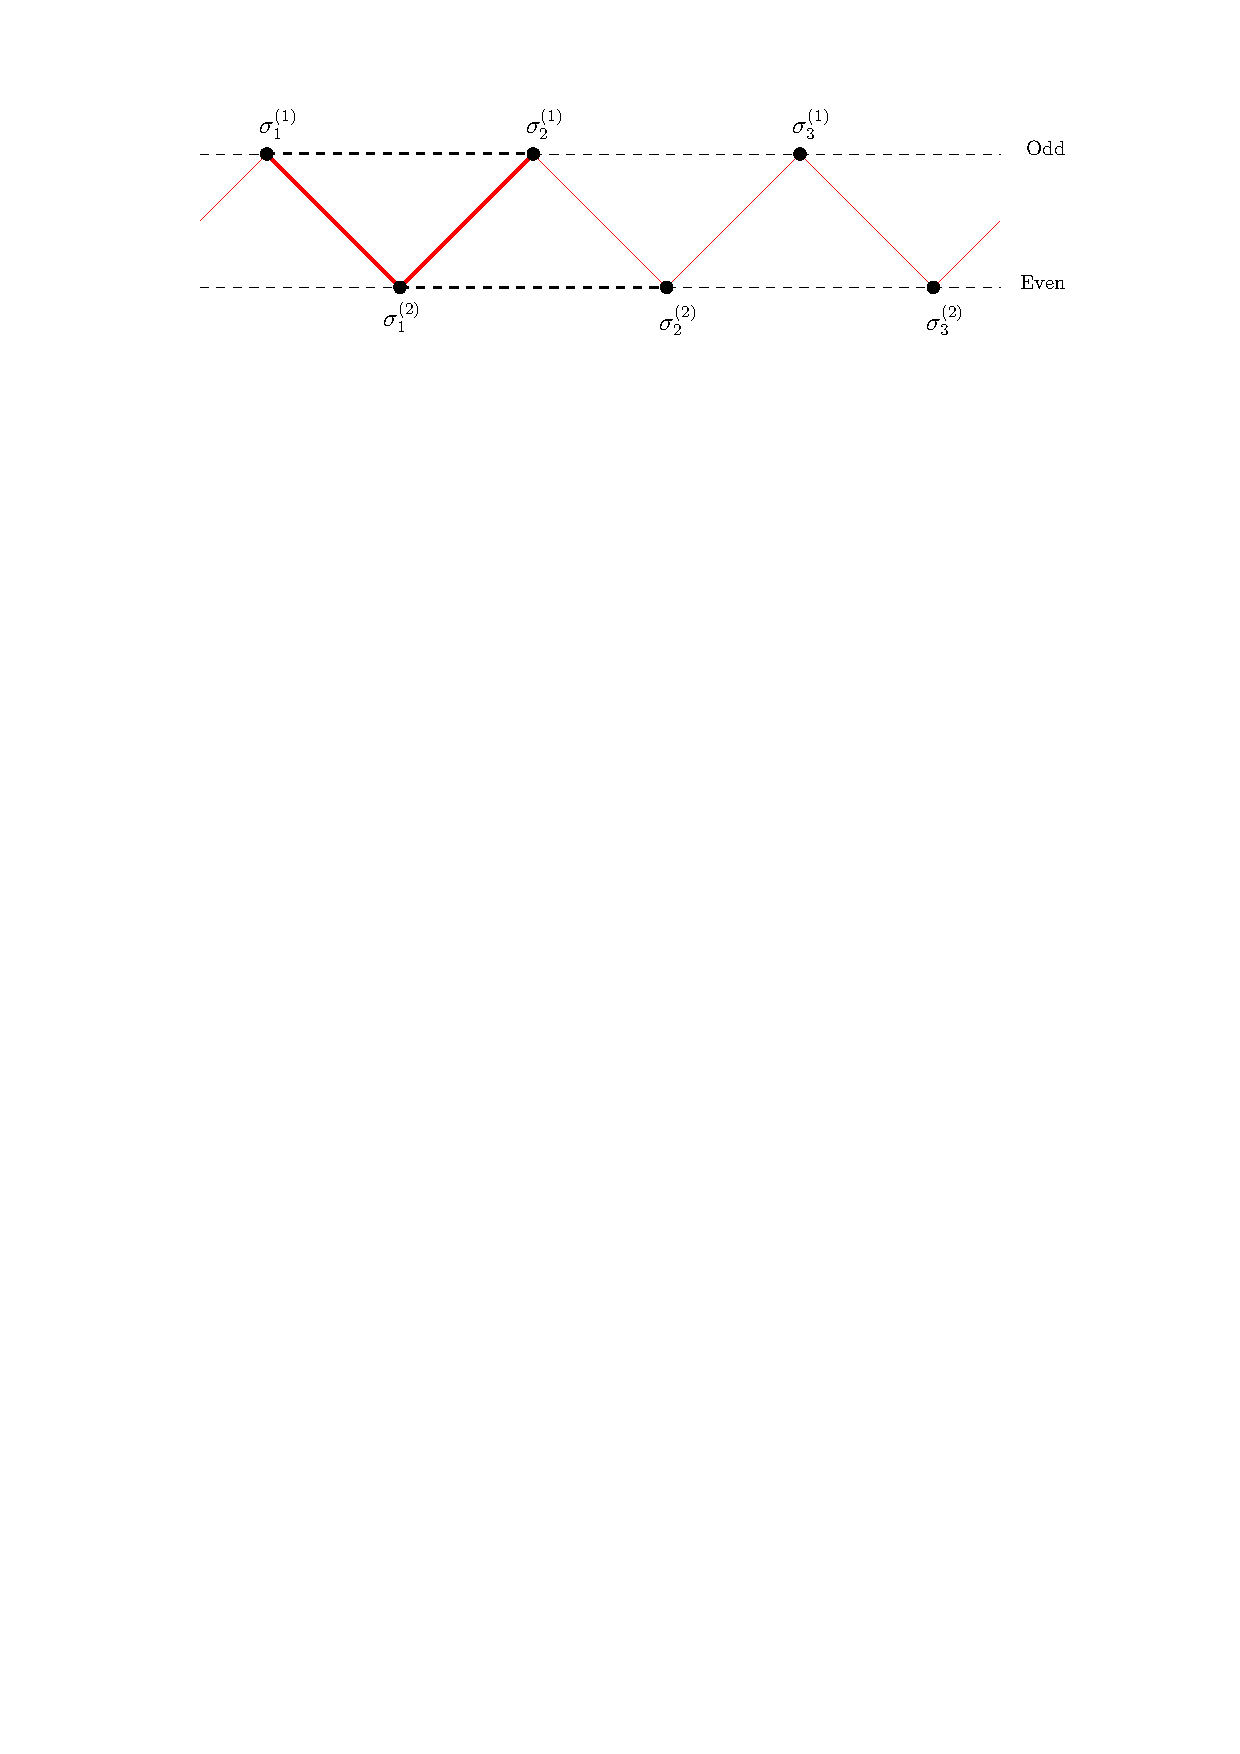
\includegraphics{nnn.pdf}
    \caption{Graphical representation of the IM model with both nearest-neighbour and next-to-nearest-neighbour interactions. Spins are represented as black dots, and ordered in two lines (chains) depending on their \textit{parity}. The red continuous lines connect nearest-neighbours ($J_1$ terms), while the black dashed lines join next-to-nearest-neighbours ($J_2$ terms). The interactions described by the first term ($x=1$) of (\ref{eqn:h-parity}) are highlighted in bold.\label{fig:next-nearest-model}}
\end{figure}


The two \textit{multi}-indices of the transfer matrix will be $(\sigma_x^{(1)}, \sigma_x^{(2)})$ and $(\sigma_{x+1}^{(1)}, \sigma_{x+1}^{(2)})$, and so we need all terms to contain both of them:

\begin{align*}
    \mathcal{H}(\bm{\sigma}) &= 
    -\Big[
    \frac{J_1}{\textcolor{Red}{2}} \sum_{x=1}^{N/2} [\sigma_x^{(1)} \sigma_x^{(2)} + 2\sigma_x^{(2)} \sigma_{x+1}^{(1)} + \textcolor{Red}{\sigma_{x+1}^{(1)} \sigma_{x+1}^{(2)}}] +   
    J_{2} \sum_{x=1}^{N/2} [\sigma_x^{(1)} \sigma_{x+1}^{(1)} + \sigma_x^{(2)} \sigma_{x+1}^{(2)}] +\\
    &\quad\>\>\,+ \frac{B}{\textcolor{Red}{2}} \sum_{x=1}^{N/2}[\sigma_x^{(1)} + \sigma_x^{(2)} + \textcolor{Red}{\sigma_{x+1}^{(1)} + \sigma_{x+1}^{(2)}} ] \Big]
\end{align*}

The partition function is given by:
\begin{align*}
    Z &= \sum_{\{\bm{\sigma}\}} e^{-\beta \mathcal{H}(\bm{\sigma})} = \sum_{\mathclap{\substack{\sigma^{(1)}_1=\pm 1\\\sigma^{(2)}_1 = \pm 1}}}\quad \cdots \quad\sum_{\mathclap{\substack{\sigma^{(1)}_{N/2}=\pm 1\\\sigma^{(2)}_{N/2} = \pm 1}}}\quad \prod_{i=1}^{N/2} \exp \Bigg(\frac{K_1}{2}\Big[\sigma_x^{(1)} \sigma_x^{(2)} + 2\sigma_x^{(2)} \sigma_{x+1}^{(1)} + \sigma_{x+1}^{(1)} \sigma_{x+1}^{(2)}\Big] \\
    &\quad\> K_2 \Big[\sigma_x^{(1)} \sigma_{x+1}^{(1)} + \sigma_x^{(2)} \sigma_{x+1}^{(2)}\Big] + \frac{B}{2} \Big[\sigma_x^{(1)} + \sigma_x^{(2)} + \sigma_{x+1}^{(1)} + \sigma_{x+1}^{(2)} \Big] 
    \Bigg)
\end{align*}

The exponential term is one entry of a $4\times 4$ transfer matrix $\mathrm{T}$:
\begin{align*}
    \mathrm{T}_{(\sigma_x^{(1)}, \sigma_x^{(2)}), (\sigma_{x+1}^{(1)}, \sigma_{x+1}^{(2)})}
\end{align*}
By mapping $\sigma_x = \pm 1 \to \{0,1\}$, each \q{multi-index} is a binary number, defining a position in the matrix. For example, when $\sigma_x^{(1)} = \sigma_{x}^{(2)} = \sigma_{x+1}^{(1)} = \sigma_{x+1}^{(2)} = +1$, the matrix entry will be $\mathrm{T}_{(1,1),(1,1)} \equiv \mathrm{T}_{4,4}$. In this way, the sum of the product of exponentials can be interpreted as a \textit{matrix product}, leading to:
\begin{align*}
    Z = \operatorname{Tr}(\mathrm{T}^{N/2}) 
\end{align*}%Not so sure

%Source: https://inis.iaea.org/collection/NCLCollectionStore/_Public/27/020/27020481.pdf

\end{document}
